\documentclass[12pt,a4paper,final,twoside]{stylevk}
% \usepackage[dvips]{graphicx}
\usepackage{times} 
\usepackage[pdftex]{graphicx}
%
% ToDo List for the User's Guide
%
% Issue 765: FDS+Evac, Documentation of EVAC_DT_FLOWFIELD vs EVAC_DT_MAX
%            Clarify, make a separate paragraph, where the time steps are
%            discussed.
%
% Issue 766: FDS+Evac, Documentation, Clarify input: FLOW_FIELD_ID
%            Done.
%
%
\usepackage[T1]{fontenc}
\usepackage[latin1]{inputenc}
\usepackage[english]{babel}
\usepackage{fancyhdr}
\usepackage{upquote}
% upquote works only for verbatim. \char"0D gives correct quote
% character elsewhere.
%
\usepackage{amsmath}
\usepackage{amssymb}
\usepackage{amsfonts}
\usepackage{array,eqnarray}

% Next is not working for T.K.
% \usepackage{hyperref}
%
% \usepackage{color}
% \definecolor{linknavy}{rgb}{0,0,0.50196}
% \definecolor{linkred}{rgb}{1,0,0}
% \definecolor{linkblue}{rgb}{0,0,1}

% \usepackage{caption}
% \usepackage{graphpap}
% \usepackage{rotating}
%%% \usepackage{epsfig,psfrag}
%\usepackage{wrapfig}
%\usepackage{picins}
\usepackage{geometry}
\usepackage{tabularx}
\usepackage{longtable}
\usepackage{lscape}
\usepackage{makeidx} % Create index at end of document
% \usepackage[nottoc,notlof,notlot]{tocbibind} % Put the bibliography and index in the ToC
\usepackage{float}
\usepackage{lastpage} % Automatic last page number reference.
% \usepackage{indentfirst} 
%

% Page layout for the VTT Working Papers (A4 paper)
% top margin 3.0 cm (including top header 1.0 cm)
% bottom margin 3.0 cm + page number (4.0 cm)
% left + right margins 3.0 cm 
%
% Beginning of 2009: VTT Working Papers is in A4 format:
% Main chapters:
% Top margin 5.2 cm, top header 3.5 cm
% Bottom margin 4.8 cm, bottom label 3.5 cm, page number at center
% Header:  Bold Arial 10 pt, 12 pt line height
% Main text: 12 pt Times New Roman, 16 pt line height
% Body text first indent 0.37 cm
%
\setlength{\paperheight}{297mm}
\setlength{\paperwidth}{210mm}
\setlength{\hoffset}{0mm}
\setlength{\voffset}{0mm}

\setlength{\topmargin}{0.0cm}
\setlength{\headheight}{12pt}
\setlength{\headsep}{16pt}
\setlength{\textheight}{227mm}
\setlength{\footskip}{22mm}

\setlength{\textwidth}{150mm}
\setlength{\oddsidemargin}{4.6mm}
\setlength{\evensidemargin}{4.6mm}

\setlength{\parindent}{3.7mm}
\setlength{\parskip}{0pt}
% \setlength{\parskip}{16.0pt plus 3.5pt minus 1.0pt}
\setlength{\baselineskip}{16.0pt plus 3.5pt minus 1.0pt}

% Heading styles for the VTT Working Papers (A4 paper)
% These are (re)defined in stylevk.
% Next are for the new A4 Working Papers 2009
% Heading 1: Arial 18pt bold (large) (Arial ==> textsf Sans Serif)
%            riviv�li 20 pt, 130pt tyhj�� tilaa ennen otsikkoa
%            otsikon j�lkeen 16pt tyhj��
% Heading 2: Arial 14pt bold, 16pt riviv�li, 20pt tyhj�� ennen, 14pt j�lkeen
% Heading 3: Arial 12pt bold, 16pt riviv�li, 18pt tyhj�� ennen, 14pt j�lkeen
% Heading 4: Arial 12pt, 16pt riviv�li, 18pt tyhj�� ennen, 12pt j�lkeen
% Contents: Arial 18pt bold
% Abstract: Arial 18pt bold, riviv�li 20pt, 60pt tyhj�� ennen, 12pt
%           j�lkeen (sis.luetteloon 1. tason otsikkona)
% alkusanojen otsikko: kuten 1. tason otsikko
% sis.luettelon otsikko: kuten 1. tason otsikko, sen j�lkeen 24pt tyhj��
% Acknowledgements: Heading 1
% References: Heading 1, text: 10pt, 13pt riviv�li, 1.5 cm riippuva
%             sisennys, kappaleen j�lkeen 13pt tyhj��
% Captions: Arial 10pt, 13pt riviv�li, 12pt tyhj�� ennen, 16pt j�lkeen


% \renewcommand{\refname}{\textbf{\normalsize REFERENCES}}
% \renewcommand{\figurename}{\normalsize FIGURE}
% \renewcommand{\tablename}{\normalsize TABLE}
% \renewcommand{\refname}{\normalsize REFERENCES}

%% The maximum number of floats on a page
\setcounter{totalnumber}{3}
%% The level of section numbering
\setcounter{secnumdepth}{3}

% How to use the low level font commands:
% Title: Bold, 14 pt, Times Roman
% {\fontsize{14}{17} \selectfont \bf FDS+Evac: Model}

% \pagestyle{plain}
\pagestyle{headings}

\begin{document}

%% % \bibliographystyle{unsrt}


\newcommand{\Timts}[1]{\textnormal{\texttt{\textsl{#1}}}}
\newcommand{\Timtt}[1]{{\tt{#1}}}
%% % \newcommand{\Timtt}[1]{\textnormal{\texttt{#1}}}
%% % \renewcommand\Large{\@setfontsize\Large\@xxxviiipt{23}}
%% %\let`\textasciigrave
%% %\let'\textquotesingle
\newcommand{\QS}{\hbox{\textquotesingle}}

\fancyhead{}
\fancyfoot[C]{\today}
\renewcommand{\headrulewidth}{0.0pt}
\renewcommand{\footrulewidth}{0.0pt}

\begin{titlepage}

  \thispagestyle{fancy}

  \begin{center}

    VTT Technical Research Centre of Finland

    \vspace{90mm}

    { \normalfont\fontsize{28}{42}\selectfont\bfseries\sffamily
      Fire Dynamics Simulator with Evacuation: FDS+Evac
    }

    \vspace{6mm}

    { \normalfont\fontsize{22}{28}\selectfont\bfseries\sffamily
      Technical Reference and User's Guide }

    { \normalfont\fontsize{14}{18}\selectfont\sffamily
      (FDS 5.3.1, Evac 2.1.2) }

    \vspace{15mm}

    { \normalfont\fontsize{14}{18}\selectfont\sffamily
      Timo Korhonen and Simo Hostikka }

    \vspace{3mm}

    { \normalfont\fontsize{12}{16}\selectfont\sffamily
      VTT}

  \end{center}


\vspace{2cm}
    

\end{titlepage}

\setcounter{page}{4}

\newpage


\chapter*{Preface}
\addcontentsline{toc}{chapter}{Preface}

This document describes how to simulate human egress using the
evacuation module, FDS+Evac, developed at VTT Technical Research
Centre of Finland, which is fully embedded in Fire Dynamics Simulator
(FDS).  This manual applies to the FDS+Evac version is 2.1.1, which is
embedded in the current FDS version 5.3.0.  The most up to date
version of this manual can be obtained from the FDS+Evac web page at
\texttt{http://www.vtt.fi/}\linebreak[4]\texttt{fdsevac/}.

The FDS+Evac Technical Reference and User's Guide does not contain
information on how to operate FDS nor Smokeview, the companion
visualisation programme for FDS.  Their full capabilities are
described in the ``Fire Dynamics Simulator (Version 5) User's
Guide''~\cite{FDS_UserGuide} and the ``User's Guide for Smokeview
Version 5''~\cite{SV_UserGuide}.

Certain commercial entities, equipment, or materials may be identified
in this document in order to describe an experimental procedure or
concept adequately.  Such identification is not intended to imply
recommendation or endorsement by VTT Technical Research Centre of
Finland, nor is it intended to imply that the entities, materials, or
equipment are necessarily the best available for the purpose.

\newpage


\chapter*{Disclaimer}
\addcontentsline{toc}{chapter}{Disclaimer}

VTT Technical Research Centre of Finland makes no warranty, expressed
or implied, to users of FDS+Evac, and accepts no responsibility for
its use.  Users of FDS+Evac assume sole responsibility for determining
the appropriateness of its use in any particular application; for any
conclusions drawn from the results of its use; and for any actions
taken or not taken as a result of analyses performed using these
tools.

Users are warned that FDS+Evac is intended for use only by those
competent in the fields of fire and evacuation simulation, and is
intended only to supplement the informed judgement of the qualified
user.  The software package is a computer model that may or may not
have predictive capability when applied to a specific set of factual
circumstances.  Lack of accurate predictions by the model could lead
to erroneous conclusions with regard to life safety.  All results
should be evaluated by an informed user.


\clearpage

\newpage


\tableofcontents

\newpage

\chapter{Introduction}\label{Sec_Intro}

\noindent This document describes how to simulate human egress using the Fire
Dynamics Simulator (FDS)~\cite{FDS_Manual, FDS_UserGuide,
  FDS_VVGuide1, FDS_VVGuide2}, and in particular, the evacuation
module~\cite{Korhonen05, Korhonen07a, Korhonen07b, Korhonen08a,
  Korhonen08b}.  This combined fire and evacuation simulation program
is called FDS+Evac in this document.  FDS+Evac allows simultaneous
simulation of the fire and evacuation processes.  It can also be
used to simulate only the human egress process without any fire
effects, \emph{e.g.}, a fire drill.

FDS+Evac treats each evacuee as a separate entity, or an 'agent',
which has its own personal properties and escape strategies.  The
movement of the agents is simulated using two-dimensional planes
representing the floors of buildings.  The basic algorithm behind the
egress movement solves an equation of motion for each agent in a
continuous 2D space and time, \emph{i.e.}, FDS+Evac is doing some kind
of an artificial molecular dynamics for the agents.  The forces acting
on the agents consist of both physical forces, such as contact forces
and gravity, and psychological forces exerted by the environment and
other agents.  The model behind the movement algorithm is the social
force model introduced by Helbing's group~\cite{Helbing95, Helbing00,
  Helbing02, Werner03}.  A modification of the model to describe
better the shape of the human body was introduced by Langston \emph{et
  al.}~\cite{Langston06}.

This chapter contains some general information on FDS+Evac.  In
Chapter 2, the model documentation is summarised. Chapter 3 presents
the theoretical model behind the agent movement algorithm and details
on the implementation.  Chapter 4 is dedicated to various verification
tests of the programme and Chapter 5 deals with the sensitivity of the
model to the model parameters.  In Chapter 6, FDS+Evac is validated
by comparing to other evacuation calculation methods and experimental
results.  Chapters 7--11 contain the user's guide, where the
inputs of FDS+Evac are explained.

The user of FDS+Evac should read carefully every chapter of this
manual before starting to use the programme.  The knowledge on the
theoretical method is needed in order to build up the model
correctly.  It also helps making the judgement on the applicability
and reliability of the programme in the application in question.
Because the evacuation calculation is implemented as a module of FDS,
the reader is recommended to read first the User's Guide of FDS and
learn how to do fire simulations.  Even if the user wants to run the
programme without fire, she/he should be acquainted with the FDS in
order to build up the simulation geometry and running the FDS
simulations.


\section{Getting Started}\label{Sec_GetStart}

\noindent The evacuation module is embedded inside the FDS.  Thus, the
running of FDS+Evac evacuation simulation is done similarly as an
ordinary FDS fire simulation.  See the FDS User's
Guide~\cite{FDS_UserGuide} for details.  FDS+Evac results can be
visualised using the Smokeview~\cite{SV_UserGuide} programme. Also,
the computer hardware requirements are similar with FDS.  The FDS fire
calculation can be run parallel by using the MPI version of FDS, but
the evacuation part is always calculated as a single thread.

The evacuation module, FDS+Evac, is embedded in the FDS 5.3,
which can be obtained from the URL
\begin{verbatim}
http://fire.nist.gov/fds/
\end{verbatim}
Download the latest version of FDS-Smokeview installation package and
install it.  Check if there exists more recent maintenance releases of
the executables.  The resulting FDS executables are also the
executables of the evacuation calculation module.  The source codes
can also be obtained via the FDS-SMV web pages.


The home page of FDS+Evac is 
\begin{verbatim}
http://www.vtt.fi/fdsevac/
\end{verbatim}
This page contains the most recent version of this combined Technical
Reference and User's Guide of FDS+Evac and some examples on the use of
FDS+Evac.  This web site is also used to store the validation and
verification test cases including the input files.  This (printed)
manual refers to FDS 5.3.0 + Evac 2.1.1.



\section{Features of Limited Functionality}\label{Sec_SpecFeatures}

\noindent All the intended features of FDS+Evac are not yet fully functional.
For now, FDS+Evac is best suited for doing calculations in buildings,
whose floors are mainly horizontal.  Sports halls with spectator
stands or concert halls can also be modelled if their geometry is not
too complicated, but the user should note that simulations in inclined
geometries have not yet been validated.  It is also assumed that the
different levels of the building are separated from each other,
\emph{i.e.}, they are connected to each other by stairs, escalators,
doors, and similar objects.  Note, that FDS+Evac does not support
the use of elevators during evacuation process.  Wide stairs or
inclines can also be used to connect different floors, but this is not
as straightforward as to use the default staircase model.  There are
no merging flows allowed in the default staircase model, so FDS+Evac
is not yet easy to use for tall buildings.  The default staircase
algorithm is still very simple and it should not be trusted too much
if the stairs get crowded.  At this point this is not a major problem,
because there are no merging flows in the staircase model,
\emph{i.e.}, the exit door restricts the flow to the staircase quite
efficiently.  If merging flows in staircases are needed then the
detailed geometry of the staircase should be modelled, but this is not
usually very practical way of doing things.  See the example case
``\texttt{Stairs.fds}'' on the FDS+Evac web pages.

The evacuation calculation needs, in addition to the fire calculation
meshes, its own 2D evacuation meshes.  If no fire related data is
needed in the evacuation calculation then there are no need for fire
meshes and FDS+Evac can be run in a ``fire drill'' mode.  Evacuation
meshes should not be too fine, because then one might face problems
with the evacuation flow fields, which are used to guide the agents
towards the exits.  This difficulty can be addressed by an experience
user, but an easier way is always to use evacuation meshes, which are
not too fine.  Usually mesh cell sizes 0.25~m or larger can be used
without any problems.  For example, if you have 1.2~m wide doors you
could use 0.3~m, 0.6~m, or 1.2~m cell spacing depending on how
detailed geometry is needed.  Note, that Smokeview does not yet fully
support the evacuation calculation, \em e.g.\em, the positions of
doors, stairs and other evacuation objects are not shown by Smokeview.
Note also that the spaces, where agents are allowed to move, should be
at least about 0.7~m wide, because FDS+Evac is not able to move agents
in narrower exit paths correctly.  The user should check the
evacuation geometry by using the Smokeview programme and make sure
that the ``holes'' in the evacuation geometry are not too narrow.  The
best way of seeing the evacuation geometry is to do a calculation
without any fire mesh definitions.  Then the Smokeview shows just the
evacuation geometry.  It is a good practice to construct first the FDS
fire calculation input file and do a short test run.  After this one
can add the evacuation meshes to the calculation and deactivate the
fire meshes, \emph{i.e.,} try to simulate (and see) just the
evacuation part of the calculation.  When the evacuation part of the
input file seems to be working as it should then a full fire +
evacuation calculation could be done.

Note that while the FDS fire simulations can use time dependent
geometry elements, such as obstacles and holes, which are created and
removed by special control devices, the evacuation geometry does not
support the time dependent geometries.  For evacuation, the initial
geometry is always used for the whole duration of the simulation, but
the user can give time dependent information on the usability of the
doors for the door selection algorithm.

For now, the number of agents placed in the same main evacuation mesh
is limited.  The programme stops and writes out an error message if
more than 10~000 agents are tried to place on the same evacuation mesh.
Usually, one main evacuation mesh extends over a whole floor of the
building.  Several main evacuation meshes may coexist, \emph{e.g.},
the different floors of the building, and the total number of agents
is not restricted by the programme.  The available computer memory is
the only factor limiting the total number of agents.  However, the
calculation is going to be very CPU expensive if there are more than a
few thousands agents in the same evacuation mesh.

The initial density of agents cannot be much larger than 4 persons per
square metre.  In cases of high human density, the simulation may
require a couple of initialisation trials, because the initial
positions of agents are generated randomly. If FDS+Evac cannot place
agents on their initial positions, an error message ``\texttt{ERROR: FDS
improperly set up.}'' is printed on the standard error channel and more
information is printed on the diagnostic output file of the evacuation
calculation.

FDS+Evac enables coupled fire and evacuation simulations.  The smoke
and gas concentrations from the fire calculation affect the movement
and decision making of the evacuating humans.  In principle, the
coupling could also be made to the other direction, \emph{i.e.},
humans could influence the fire calculation, \emph{e.g.}, by opening
doors, but this feature is not yet implemented in FDS+Evac.  Gas phase
concentrations of $\mathrm{O_2}$, $\mathrm{CO_2}$, and $\mathrm{CO}$
are used to calculate Purser's Fractional Effective Dose (FED)
index~\cite{Purser95}, indicating the human incapacitation.  Smoke
density is used both to slow down the walking speeds of the agents and
to affect the exit selection algorithm of the agents.  Smoke density
can also be used to speed up the detection the fire, but it should be
kept in mind that human nose is a very delicate instrument and the
levels of smoke concentration needed for a smoke sensing may be below
the accuracy of the current FDS predictions.  Note that the effects of
radiation and gas temperature on agents are not yet implemented in the
programme, so agents do not try to avoid a fire if the user does not
explicitly define the evacuation geometry to take this in to account.

The evacuation part of the FDS+Evac is stochastic, \emph{i.e.}, it
uses random numbers to generate the initial positions and properties
of the agents.  In addition, there is a small random force on each
agent's equation of motion.  Thus, same results are not obtained for a
given input file if multiple simulations are done.  For this reason,
one should always do a dozen or so egress simulations to see the
variation of the results.  To speed up this process, several egress
calculation can be done per one fire simulation and the calculation of
the evacuation flow fields used to guide agent movement need to be
calculated only once to each given geometry.

The present version of FDS+Evac does not use computer memory optimally
and does not fully support parallel CPU calculations for the
evacuation part.  In later versions of the programme, the memory usage
will be optimised.  Currently, an efficient use of the computer memory
requires that the evacuation meshes are made as small as possible and
as few obstacles as possible are placed in the calculation.  For now,
if FDS+Evac calculation takes too much memory, the user must increase
the amount of available memory.  This may require switching from a 32
bit to a 64 bit operating system, because the evacuation meshes can
not be distributed over many different processors/computers unlike the
FDS fire meshes using the MPI version of the FDS executable.



\section{Most recent changes}\label{Sec_RecentChanges}

\noindent Below is a short description of the changes made to the different
versions of FDS+Evac.  For a full change log, the reader is asked to
consult the \texttt{Readme.txt} file, which is on the FDS+Evac web
page.


\subsection{Most recent changes, version 2.1.1 vs 2.1.0}\label{Sec_211vs210}

The namelist objects \Timtt{EXIT}, \Timtt{DOOR}, and \Timtt{ENTR} have
their \Timtt{XB} fitted to the underlying grid just like the ordinary
geometric objects in FDS fire calculation meshes, \emph{e.g.},
\Timtt{OBST} and \Timtt{VENT} namelists.  Note, that the \Timtt{EVAC},
\Timtt{EVHO}, and \Timtt{EVSS} namelists are not (yet) fitted to the
grid.

\subsection{Most recent changes, version 2.1.0 vs 2.0.0}\label{Sec_210vs200}

The version 2.0.0 demanded that a door should be defined such that it
is slightly inside a wall, see Figure~\ref{Fig_DoorGeom}.  One had to
define a small hole in the wall, where an exit (or a door) was placed.
This is not anymore necessary in version 2.1.0.  The ``outflow'' vent
and the exit door can be placed directly at the wall surface. 

In the earlier versions of FDS+Evac (2.0.0 and earlier) it was assumed
that all obstacles in the computational geometry were at least one
grid cell thick, \emph{i.e.}, \Timtt{THICKEN=.TRUE.} was forced on
the evacuation meshes.  Now this is not anymore forced, so one can use
thin obstacles for the evacuation geometry, but the user should keep
in mind that one can not place a VENT on a zero thick obstacle.

The keywords \Timtt{AVATAR\_RGB} and/or \Timtt{AVATAR\_COLOR} are used
to give the colour of the agents shown in Smokeview on the \Timtt{EVAC}
and \Timtt{ENTR} namelists instead of the \Timtt{QUANTITY} keyword.
Similar change is done for the namelists \Timtt{DOOR} and
\Timtt{EXIT}, where the keywords \Timtt{RGB} and/or \Timtt{COLOR} are
now used to give the colouring information instead of the
\Timtt{COLOR\_INDEX} keyword.

%
\begin{figure}[!tb]
  \centerline{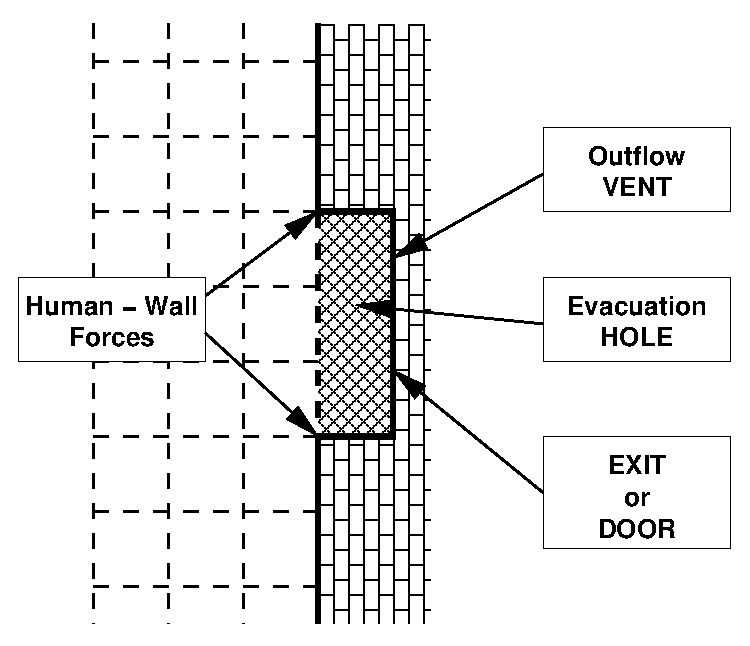
\includegraphics[clip=true,
    width=75mm]{FIGURES/door_geometry2}}
  \caption{How to make an exit or a door.}\label{Fig_DoorGeom} 
\end{figure}
%

\section{Intended Use of FDS+Evac}\label{Sec_IntUsers}

\noindent FDS+Evac is primarily a research tool for studying evacuation processes
in buildings.  While it seems to produce similar egress flows as found
in the literature (both experimental and other simulation tools) it
is not yet fully validated.  Thus, its use as an engineering tool
needs further considerations.  It is suggested that FDS+Evac is used
together with some other (well) validated egress programme to study
evacuation.  If the two (or more) methods give similar results then
the predictions of the computational modelling should be quite good.

It is not the purpose of this document to give instructions on how to
define the egress scenarios for the design purposes. Fire regulators
and designers should agree on the relevant scenarios and acceptance
criteria before any design by the engineering methods.


\clearpage

\newpage

\chapter{Model Documentation}\label{Sec_ModelDef}

\noindent This chapter provides a short description of the evacuation module of
the Fire Dynamics Simulator (FDS).  Detailed information about FDS can
be found in its documentation~\cite{FDS_Manual, FDS_UserGuide,
  FDS_VVGuide1, FDS_VVGuide2} and more detailed information about the
evacuation algorithm and its features can be found in the next
chapters.  Smokeview, the companion programme of FDS, is used to
visualise the results of FDS and FDS+Evac calculations and information
on its properties and how to use it can be found on its
documentation~\cite{SV_UserGuide}.



\section{Name and Development Environment}

\noindent The underlying fire simulation programme, Fire Dynamics Simulator
(FDS), is a computational fluid dynamics (CFD) model of fire-driven
fluid flow.  FDS is written using Fortran 90 programming language.
The companion programme Smokeview, written in C/OpenGL programming
languages, is used for graphical presentation of the simulation
results. The evacuation calculation module developed at VTT Technical
Research Centre of Finland (VTT) is implemented as subroutines of FDS
and these subroutines together with the FDS are called as FDS+Evac.
Since the version 5 of FDS, the program development and maintenance
has utilised a version control system (SVN).  The source code is
maintained at a public domain server.\footnote{The server is hosted by
  Google Code (http://code.google.com/p/fds-smv/)} Changes in the
version numbers correspond to major changes in the physical models or
input parameters.  For minor changes and bug fixes, incremental
versions are released, referenced according to fractions of the
integer version numbers.  In addition, day-to-day bug fixes made in
response to user feedback are referenced by a compilation date and a
SVN revision number that are printed at the top of the diagnostic
output file.  The latest official release version of FDS is obtainable
on the web site {\tt http://fire.nist.gov/fds/}.  The latest
documentation on the evacuation part of FDS+Evac can be found on the
web page {\tt http://www.vtt.fi/fdsevac/}.

\section{Type of the Model}

\noindent FDS+Evac is a combined agent-based egress calculation model and a
Computational Fluid Dynamics (CFD) model of fire-driven fluid flow,
where the fire and egress parts are interacting.  FDS+Evac can also be
used just to calculate the egress problem without any fire-driven
fluid flow calculation, \emph{e.g.}, it can be used to simulate fire
drills.  FDS+Evac models the egress of the agents using continuous
space and time, but the building geometry is fitted to the underlying
rectilinear mesh.  FDS+Evac uses simple rules and artificial
intelligence to model the exit selection processes of the evacuees.

\section{Model Developers}

\noindent The evacuation module of FDS was developed and its currently
maintained by the VTT Technical Research Centre of Finland.  A
substantial contribution to the implementation of the evacuation
calculation as a module of FDS was made by the Fire Research Division
in the Building and Fire Research Laboratory (BFRL) at the National
Institute of Standards and Technology (NIST).  Additional contributors
and co-workers are cited in the Acknowledgements.

\section{Relevant Publications}

\noindent Each version of FDS+Evac is documented by this publication -- the
FDS+Evac Technical Reference and User's Guide.  The User's Guide part
of the publication explains the mechanics of using the computer
programme.  The Technical Reference Guide part provides the theory and
the details of the algorithms, plus a description of the verification
and validation studies and details about the many parameters of the
evacuation model and their default values.  This section contains also
a throughout study of the effects of the model parameters on the
calculated egress flows.  Note that the most up to date verification
and validation results are on the FDS+Evac web page.  This manual is
not updated as frequently as the web page and the web page will
contain more example cases than this manual.

The model behind the movement algorithm of FDS+Evac was introduced by
Helbing's group~\cite{Helbing95,Helbing00,Helbing02,Werner03}.  The
implementation of this algorithm inside the FDS program environment
was introduced by Korhonen \emph{et al.}~\cite{Korhonen05}.  Later the
model was modified along the lines given in the paper by Langston
\emph{et al.}~\cite{Langston06} to a three circle representation of
humans by Korhonen \emph{et al.}~\cite{Korhonen07a, Korhonen07b,
  Korhonen08a, Korhonen08b}.

\section{Input Data Required to Run the Model}

\noindent All of the input parameters required by the evacuation part of
FDS+Evac to describe a particular scenario are conveyed via one text
file, which is the same one that is used for FDS, created by the user.
For the fire-driven fluid flow related parameters, see the FDS
documentation~\cite{FDS_UserGuide}.  The input file of FDS+Evac is
such that it can be used with just minor modifications (commenting out
the evacuation meshes) to run an ordinary FDS calculation without
evacuation calculation.  Same is true for the other way also,
\emph{i.e.}, by commenting out the fire meshes one can make easily
test runs to see that the construction of the evacuation calculation
part is done correctly.

A complete description of the input parameters required by the
evacuation module of FDS can be found in the User's Guide part of this
document.

\section{Model Results}

\noindent FDS+Evac computes the position, the velocity, and the dose of toxic
gases of each agent inside the computational domain at each discrete
time step.  The movement of agents can be visualised using the
Smokeview programme~\cite{SV_UserGuide}.  The number of agents gone
through different parts of the evacuation scenario as well as the
number of agents in different evacuation nodes are saved in simple,
comma-delimited text file, that can be plotted using a spreadsheet
programme.  Some additional, quite detailed, information are written
to the diagnostic evacuation text file including the initial positions
and properties of the agents.

\section{Uses and Limitations}\label{Sec_UsesAndLimit}

\noindent Although FDS+Evac can address many egress scenarios, there are
limitations in all of its algorithms.  The most prominent
limitations are listed below.

\underline{Geometry:} The efficiency of FDS is due to the simplicity
of its rectilinear numerical mesh.  This can be a limitation in some
situations, where certain geometric features do not conform to the
rectangular mesh.  The numerical meshes used by the agent movement
algorithm of FDS+Evac are two-dimensional cut-offs of the FDS fire
meshes, thus the same limitations apply to the evacuation part of the
code.  The present version of the evacuation module can also treat
inclines, like wide stairs and spectator stands, which are along the
$x$ or $y$ direction of the underlying rectangular mesh.  The grid
cell size determines the finest details of the building geometry,
which can be modelled by the programme, \emph{e.g.}, the widths of the
doors are integral multiples of the grid cell sizes.

\underline{Reduced Visibility:} The smoke concentration calculated by
the FDS is used to slow down the walking speeds of the agents using
the results of the experiment by Frantzich and
Nilsson~\cite{Frantzich03}, where larger smoke concentrations were used
than in the experiments by Jin~\cite{Jin78}.  The scatter of the
experimental results is wide and new experimental results would be
more than welcome.  Note also that in reality there are differences
between individuals in this respect, but the present version of the
programme uses average values for each agent.  The default model for
stairs does not include the option for agents to turn back when the
smoke concentration becomes too high.

\underline{Incapacitation:} The incapacitation model is the FED
concept introduced by Purser~\cite{Purser95}, but the large scatter
between different humans is not taken into account in the current
version of the programme.  Whereas FDS is doing well for the smoke
transport and the prediction of O${}_2$ levels, it does much worse on
the prediction of the CO concentration.  In the standard mixture
fraction model of FDS, the amount of CO produced is mainly decided by
the user inputs.  Note also, that the effect of HCN is not modelled
and that the toxic effects of CO${}_2$ are not modelled; only its
hyperventilation factor is included.

\underline{Exit Route Selection:} The exit door selection algorithm is
still a relatively simple one.  It does not include any kind of social
interactions, like herding behaviour.  The user has more or less full
control on the doors which different agents will be using.  In some
applications this can be listed as a benefit of the model, but the
requirements for user's responsibility and expertise should be
recognised.

\underline{Detection and Reaction Times:} The pre-movement time of the
evacuating humans is decided by the user input by giving distributions
for the detection and reaction times.  In addition to the detection
time given user input, the local smoke concentration can be used to
trigger the detection of a fire. Currently, the fire detection by
agents can not be connected to the control logic of FDS, \emph{e.g.}
the smoke/heat detectors in FDS fire calculation can not be used to
trigger the movement of the agents.

\underline{Applications:} There is no model for elevators in the
current version of the FDS+Evac.  Nor there is any specific objects
relevant to maritime applications.  Concert halls and sport facilities
may be difficult to model due to the limitations dictated by the
rectangular computational mesh.  There is limitation on the number of
humans per evacuation mesh (usually one mesh per one floor).  In the
present version one floor can contain at most 10~000 humans.  The
present version of FDS+Evac supports parallel calculation only for the
fire meshes, the evacuation meshes are always treated as a single
thread.  Thus, it is not possible to divide the evacuation calculation
to different processors using the parallel version of FDS5.  This sets
the upper limit on the complexity of geometry, which can be modelled
due to the available computer RAM memory.  Changing to a 64 bit
operating system and downloading the 64 bit versions of the FDS
executables the memory problems may be avoided.

\clearpage

\newpage

\chapter{Theoretical Basis for the Evacuation Model}\label{Sec_BasisModel}


\section{Introduction}

\noindent FDS+Evac treats each escaping person as an individual agent, whose
movement is treated by an equation of motion.  This approach allows
each agent to have its own personal properties and escape strategies.
Agents experience contact forces and moments as well as psychological
and motive forces and moments.  The resulting equations of motions for
the translational and rotational degrees of freedom are solved using
the methods of dissipative particle dynamics.  Thus, the model uses
continuous time and space to track the trajectories of the agents.
FDS+Evac allows the modelling of high crowd density situations and the
interaction between evacuation simulations and fire simulations.  Some
social interactions among the agents are introduced in the model.  A
reaction function model is used to select the exit routes.


Humans are modelled as agents, which are moving in a 2D geometries
representing the floors of buildings.  The size of each agent is
represented by three circles approximating the shape of the human
body, see Figure~\ref{Fig_HumanBody}, just like in the Simulex
programme~\cite{Simulex96, Thompson95a, Thompson95b, Thompson03}, in
the MASSEgress programme~\cite{Pan06}, and in the CrowdDMX
model~\cite{Langston06, Langston09}.  The body dimensions and the
unimpeded moving speeds of the default population types in FDS+Evac
are shown in Table~\ref{Table_DefaultHumans}.  The body diameters and
walking speeds are by default drawn randomly for each generated agent
from uniform distributions, whose widths are also given in the table.
The body diameter and moving speed distributions are taken to be same
as in the Simulex programme for the Male, Female, Child, and Elderly
categories.  The category Adult is just a simple superposition of the
Male and Female categories.

%
\begin{figure}[tb]
  \centerline{\includegraphics[clip=true,
    width=30mm]{FIGURES/body_shape}}
  \caption{The shape of the human body is approximated by a
    combination of three overlapping circles.  Shown are also the
    definitions of the body size variables.}\label{Fig_HumanBody}
\end{figure}
%

The existing fire simulation environment of FDS is used to minimise
the programming effort to write an egress programme.  For
visualisation, the existing Smokeview programme~\cite{SV_UserGuide}
developed at NIST is used.  Additional benefit of using FDS as the
platform of an egress model is the direct and easy access to the fire
related properties, like gas temperatures, smoke and gas densities,
and radiation levels at each point in the computational grid.  These
quantities can be used to model the behaviour of evacuating humans.
The integration of the evacuation calculation in to the fire
calculation would easily allow the evacuation calculation to change
the flow of the fire calculation, \emph{e.g.}, by allowing the
evacuees to open or close doors and windows, but this is not yet
possible with the present version of the FDS+Evac programme.


\section{Agent Movement Model}\label{Sec_MoveModel}

\noindent The method of Helbing's group is used as the starting point of the
agent movement algorithm of FDS+Evac, where a so-called ``social
force'' is introduced to keep reasonable distances to walls and other
agents, see Figure~\ref{Fig_SocForce}.  This model is shortly described
below.  For a longer description, see the papers by Helbing's
group~\cite{Helbing95, Helbing00, Helbing02, Werner03} and references
therein.  For the modification of the one-circle representation of an
agent to a three-circle one, see the papers by Langston {\em et
  al.}~\cite{Langston06} and Korhonen {\em et al.}~\cite{Korhonen07a,
  Korhonen07b, Korhonen08a, Korhonen08b}.

%
\begin{table}[b!]
\begin{center}
\caption{Unimpeded walking velocities and body dimensions in FDS+Evac.
   The offset of shoulder circles is given by $d_s = R_d - R_s$, for the
   definition of the other body size variables, $R_d$, $R_t$, $R_s$,
   see Figure~\protect\ref{Fig_HumanBody}.  The body sizes and walking
   velocities of the agents are personalised by using them from uniform
   distributions, whose rages are also given.}\label{Table_DefaultHumans}  
\vspace{12pt}
\begin{tabular}{l c c c c c}\hline\hline 
Body type & $R_d$& $R_t/R_d$ & $R_s/R_d$  & $d_s/R_d$ & Speed \\
          & (m)  & (-)   &  (-)    & (-)    & (m/s) \\ \hline
Adult     & 0.255$\pm$0.035 & 0.5882 & 0.3725 & 0.6275 & 
          1.25$\pm$0.30 \\  % +- 0.07m 0.30m/s 
Male      & 0.270$\pm$0.020 & 0.5926 & 0.3704 & 0.6296 &
          1.35$\pm$0.20 \\  % +- 0.04m 0.20m/s 
Female    & 0.240$\pm$0.020 & 0.5833 & 0.3750 & 0.6250 & 
          1.15$\pm$0.20 \\  % +- 0.04m 0.20m/s 
Child     & 0.210$\pm$0.015 & 0.5714 & 0.3333 & 0.6667 & 
          0.90$\pm$0.30 \\  % +- 0.03m 0.30m/s 
Elderly   & 0.250$\pm$0.020 & 0.6000 & 0.3600 & 0.6400 & 
          0.80$\pm$0.30 \\ \hline\hline  % +- 0.04m 0.30m/s 
\end{tabular}
\end{center}
\end{table}
%

FDS+Evac uses the laws of mechanics to follow the trajectories of the
agents during the calculation.  Each agent follows its own equation of
motion:
%
\begin{equation}\label{Eq_motion}
   m_i \frac{d^2 \mathbf{x}_i (t)}{dt^2} = \mathbf{f}_i (t)  +
  {\boldsymbol  \xi}_i (t) ~,  
\end{equation}
%
where $\mathbf{x}_i (t)$ is the position of the agent $i$ at time $t$,
$\mathbf{f}_i (t)$ is the force exerted on the agent by the
surroundings, $m_i$ is the mass, and the last term, ${\boldsymbol
  \xi}_i (t)$, is a small random fluctuation force.  The velocity of
the agent, $\mathbf{v}_i (t)$, is given by $d\mathbf{x}_i/dt$.
FDS+Evac treats agents as combination of three circles moving on a
two-dimensional plane~\cite{Langston06}.  These circles are
approximating the elliptical shape of the human body, see
Figure~\ref{Fig_HumanBody}.  The default body dimensions and the
unimpeded walking speeds of different predefined agent types of
FDS+Evac are listed in Table~\ref{Table_DefaultHumans}.  Note, that
FDS+Evac uses stochastic properties for the characteristics of the
agents.  \emph{E.g.}, the body sizes and walking velocities are drawn
from uniform distributions by default.  The ranges of these
distributions are also given in the table.


%
\begin{figure}[tb]
  \centerline{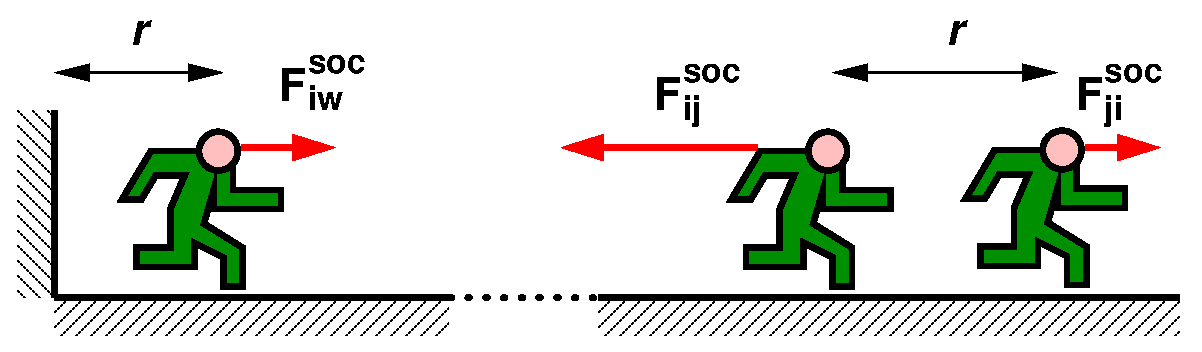
\includegraphics[clip=true,
    width=120mm]{FIGURES/voimakuvat_Poster}}
  \caption{The concept of the social force.}\label{Fig_SocForce}
\end{figure}
%

The force on the agent $i$ has many components:
%
\begin{equation}\label{Eq_force}
  \mathbf{f}_i = \frac{m_i}{\tau_i} \left( \mathbf{v}_i^0 -
    \mathbf{v}_i\right) + \sum_{j \ne i} \left( \mathbf{f}_{ij}^{soc}
    + \mathbf{f}_{ij}^{c} + \mathbf{f}_{ij}^{att} \right) + \sum_{w}
  \left( \mathbf{f}^{soc}_{iw} + \mathbf{f}^{c}_{iw} \right) + \sum_{k}
  \mathbf{f}_{ik}^{att} ~,
\end{equation}
%
where the first sum describes agent--agent interactions, the sum over
$w$ describes agent--wall interactions, and the terms in the last sum,
$\mathbf{f}_{ik}^{att}$, may be used for other agent--environment
interactions, like the fire--agent repulsion.  The first term on the
right hand side describes the motive force on the evacuating agent.
Each agent tries to walk with its own specific walking speed, $v^0_i =
\vert \mathbf{v}_i^0 \vert$, towards an exit or some other target,
whose direction is given by the direction of the field $
\mathbf{v}_i^0 $.  The relaxation time parameter $\tau_i$ sets the
strength of the motive force, which makes an agent to accelerate
towards the preferred walking speed.

The agent--agent interaction force in Eq.~\ref{Eq_force} has three
parts.  For the social force term, $\mathbf{f}_{ij}^{soc}$, the
anisotropic formula proposed by Helbing {\em et al.}~\cite{Helbing02}
is used
%
\begin{equation}\label{Eq_socialforce}
 \mathbf{f}_{ij}^{soc} = A_i e^{-(r_{ij}-d_{ij})/B_i }
 \left ( \lambda_i + (1-\lambda_i) \frac{1 + \cos \varphi_{ij}}{2}
 \right )  \mathbf{n}_{ij} ~, 
\end{equation}
%
where $r_{ij}$ is the distance between the centres of the circles
describing the agents, $d_{ij}$ is the sum of the radii of the
circles, and the vector $\mathbf{n}_{ij}$ is the unit vector pointing
from the agent $j$ to $i$.  For a three circle representation of
agents, the circles used in Eq.~\ref{Eq_socialforce} are those circles
of the two agents, which are closest to each other.  The angle
$\varphi_{ij}$ is the angle between the direction of the motion of the
agent $i$ feeling the force and the direction to the agent $j$, which
is exerting the repulsive force on the agent $i$.  The parameters
$A_i$ and $B_i$ describe the strength and spatial extent of the force,
respectively. The parameter $\lambda_i$ controls the anisotropy of the
social force. If $\lambda_i=1$, then the force is symmetric and if it
is $ 0 < \lambda_i <1$, the force is larger in front of an agent than
behind.  The psychological wall--agent interaction, $
\mathbf{f}_{ij}^{soc}$, is treated similarly, but values $A_w$, $B_w$,
and $\lambda_w$ are used for the force constants.

The physical contact force between the agents, $\mathbf{f}_{ij}^{c}$,
is given by
%
\begin{equation}\label{Eq_contactforce}
  \mathbf{f}_{ij}^{c} = \left( k_{ij} (d_{ij}-r_{ij}) + c_d \Delta
    v_{ij}^{n} \right) \mathbf{n}_{ij} + \kappa_{ij} (d_{ij}-r_{ij})\Delta
  v_{ij}^{t} \, \mathbf{t}_{ij} ~,
\end{equation}
%
where $\Delta v_{ij}^{t}$ is the difference of the tangential
velocities of the circles in contact, $\Delta v_{ij}^{n}$ is the
difference of their normal velocities, and vector $\mathbf{t}_{ij}$ is
the unit tangential vector of the contacting circles.  This force
applies only when the circles are in contact, \emph{i.e.},
$d_{ij}-r_{ij} \ge 0$.  The radial elastic force strength is given by
the force constant $k_{ij}$ and the strength of the frictional force
by the force constant $\kappa_{ij}$.  Note, that
Eq.~\ref{Eq_contactforce} contains also a physical damping force with
a damping parameter $c_d$ that was added by Langston \emph{et
  al.}~\cite{Langston06}.  The original model by Helbing {\em et al.}
did not have this force.  This parameter reflects the fact that the
collision of two humans is not an elastic one.  The physical
wall--agent interaction, $ \mathbf{f}^{c}_{iw}$, is treated similarly
and same force constants are used.

The term $\mathbf{f}_{ij}^{att}$ can be used to describe attraction
(or repulsion) between agents, like a herding behaviour or an
adult--children interaction.  It could also be used to form pairs of
agents, \emph{e.g.}, describing a fire fighter pair entering the
building.  All of the force terms in Eq.~\ref{Eq_force} are relatively
short ranged and they need a line-of-sight connection.  Longer ranged
forces could be taken in to account by changing the preferred walking
velocity field $ \mathbf{v}_i^0 $ of the agent.


%
\begin{figure}[!bt]
  \centerline{\includegraphics[ clip=true, width=100mm
  ]{FIGURES/body_shape_forces} } 
\caption{Definitions of the radial vectors $
  \mathbf{R}^c$ and $\mathbf{R}^{soc}$. }\label{Fig_BodySize}
\end{figure}
%


Equations~\ref{Eq_motion}--\ref{Eq_contactforce} describe the
translational degrees of freedom of the evacuating agents.  The
rotational degrees of freedom are treated similarly, \emph{i.e.}, each
agent has its own rotational equation of motion:
%
\begin{equation}\label{Eq_rotmotion}
   I^z_{i} \frac{d^2 \varphi_i (t)}{dt^2} = {M}^z_{i} (t)  +
  {\eta}^z_{i} (t) ~,  
\end{equation}
%
where $\varphi_i(t)$ is the angle of the agent $i$ at time $t$,
$I^z_{i}$ is the moment of inertia, ${\eta}^z_{i} (t)$, is a small
random fluctuation torque, and ${M}^z_{i} (t)$ is the total torque
exerted on the agent by its surroundings
%
\begin{equation}\label{Eq_total_torque}
  {M}^z_{i} =  {M}^c_{i} + {M}^{soc}_{i} +  {M}^{\tau}_{i} ~,
\end{equation}
%
where ${M}^c_{i}$, ${M}^{soc}_{i}$, and ${M}^{\tau}_{i}$ are the
torques of the contact, social, and motive forces, respectively.

The torque of the contact forces is calculated as
%
\begin{equation}\label{Eq_fc_torque}
  \mathbf{M}^c_{i} = \sum_{j \ne i} \left( \mathbf{R}^c_{i} \times
  \mathbf{f}_{ij}^{c} \right) ~, 
\end{equation}
%
where $\mathbf{R}^c_{i}$ is the radial vector, which points from the
centre of the agent $i$ to the point of contact, see
Figure~\ref{Fig_BodySize}.  In FDS+Evac, also the social forces exert
torques on the agents and these are given by the formula
%
\begin{equation}\label{Eq_soc_torque}
  \mathbf{M}^{soc}_{i} =  \sum_{j \ne i} \left( \mathbf{R}^{soc}_{i}
  \times \mathbf{f}_{ij}^{soc} \right) ~,
\end{equation}
%
where only the circles, which are closest to each other, are
considered.  The vector $\mathbf{R}^{soc}_{i}$ points from the centre
of the agent $i$ to the fictitious contact point of the social force,
see Figure~\ref{Fig_BodySize}.

Analogous to the motive force, the first term on the right hand
side of Eq.~\ref{Eq_force}, a motive torque is defined as
%
\begin{equation}\label{Eq_motive_torque}
  {M}^{\tau}_{i} = \frac{ I^z_{i} }{ \tau^z_{i} } \left( (\varphi_i(t)
    - \varphi^0_{i} ) \omega^0 - \omega(t) \right) = \frac{ I^z_{i}
  }{ \tau^z_{i} } \left( \tilde \omega^0_i - \omega(t) \right) ~,
\end{equation}
%
where $\omega^0 $ is the maximum target angular velocity of a turning
agent, $\omega (t)$ the current angular velocity, $\varphi_i(t)$ the
current body angle, and $\varphi^0_{i}$ is the target angle,
\emph{i.e.}, where the vector $ \mathbf{v}_i^0 $ is pointing.  The
target angular speed, $\tilde \omega^0_i$, defined in
Eq.~\ref{Eq_motive_torque} is larger when the body angle differs much
from the desired movement direction.  Langston {\em et
  al.}~\cite{Langston06} used a different formula for the motive
torque, which had a form of a spring force.  During this work, it was
noticed that a force like that will make agents to rotate around their
axis like harmonic oscillators and, thus, some angular velocity
dependent torque should be used.

In FDS+Evac method, agents are guided to exit doors by the preferred
walking direction vector field, $ \mathbf{v}_i^0$, and this field is
obtained using the flow solver of the FDS.  This vector field is
obtained as an approximate solution to a potential flow problem of a
two-dimensional incompressible fluid to the given boundary conditions,
where all walls are inert and the chosen exit door acts as a fan,
which extracts fluid out of the domain.  This method, or rather a
trick, produces a nice directional field for egress towards the chosen
exit door, see Figure~\ref{Fig_EvacFlowField}.  A field of this kind
will always guide agents to the chosen exit door.  This route will not
be the shortest one, but usually it is quite close to it.  This field
will guide more agents to the wider escape routes than on the narrower
ones due to the fact that the field is a solution to an incompressible
flow.  The analogy to an incompressible fluid flow is not a bad
starting point to find the movement directions of large human crowds.
For example, when humans are leaving a large sports or entertainment
event, they usually just follow the egress flow to the outside of the
building without much control on the process.

%
\begin{figure}[!tb]
  \centerline{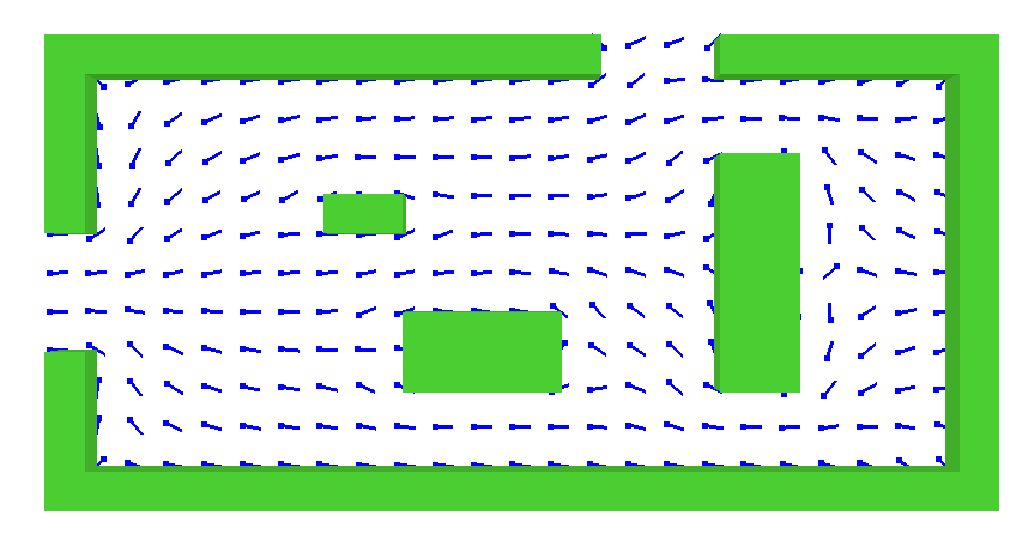
\includegraphics[clip=true,width=120mm]{FIGURES/evac_ffield}}
  \caption{A 2D flow field used to guide agents to the exit doors.  In
    this case, only the left exit has an ``outflow'' boundary
    condition, \emph{i.e.}, this fictitious agent flow field is used
    to find the left exit only.  The main evacuation mesh should also
    have an ``outflow'' boundary at the top
    exit.}\label{Fig_EvacFlowField}
\end{figure}
%

The agent movement method presented in
Eqs.~\ref{Eq_motion}--\ref{Eq_motive_torque} has many parameters.
Some of these parameters are related to physical dimensions of humans,
like $m_i$ and $I^z_{i}$, but many parameters are related to the
chosen model.  Some of these parameters are chosen to be the same as
found in the literature~\cite{Helbing00,Langston06} and some are
estimated from test calculations.  The parameters of the social force
were chosen such that the specific flows through doors and corridors
were appropriate.  The parameters of the contact forces and the
rotational degrees of freedom for the three circle representation of
the agents were selected mainly by trial and error in order to obtain
reasonably realistic looking movement.  Monte Carlo simulations were
done to see, which are the most important model parameters and further
analysis was focused on those parameters.

The first choice for the social force parameters of the agent--agent
interaction was $A_i = 2000~\textrm{N}$, $B_i = 0.04~\textrm{m}$, and
$\lambda_i = 0.5$.  For the agent--wall interaction values $A_w =
2000~\textrm{N}$, $B_w = 0.08~\textrm{m}$, and $\lambda_w = 0.2$ were
used.  It was noticed that these values are not good for congested
situations if three circles are used to describe the human body.
These parameters were modified such that the interaction strength
parameter $A$ was made velocity dependent, $A(v_i) = 2000\,
\mathrm{Max}(0.5, v_i/v^0_i)~\textrm{N}$.

For the contact force parameters, values $k_{ij} = 12 \times 10^4
~\mathrm{ \textrm{kg} \, \textrm{m}^\textrm{-2} }$, $\kappa_{ij} = 4
\times 10^4 ~\mathrm{ \textrm{kg} \, \textrm{s}^\textrm{-1}
  \textrm{m}^\textrm{-1} } $, and $c_d = 500 ~\mathrm{\textrm{kg} \,
  \textrm{s}^\textrm{-1} } $ are used both for the agent--agent and
for the agent--wall interactions.  Note that in
Eq.~\ref{Eq_contactforce} the effective elastic constant between two
agents is calculated as $k_{ij} = (k_i k_j)/(k_i+k_j)$, where $k_i$
and $k_i$ are the elastic constants of the agents, \emph{i.e.}, if the
agents have same elastic constants then $k_{i} = 2 k_{ij}$.  The
friction coefficient between two agents is simply assumed to be
independent of the agents in contact, $\kappa_{ij} = \kappa_i$.

The mass of a default male agent is $m_i = 80$~kg and its moment of
inertia was chosen to be $I^z_{i} = 4.0 ~\mathrm{ \textrm{kg} \,
  \textrm{m}^\textrm{2} }$.  For other agents, the mass and the moment
of inertia are obtained by scaling.  For the angular relaxation time
parameter, $\tau_z$, a value of 0.2~s is used.  The angular velocity
parameter $\omega^0$ has a value of $4\pi~\mathrm{
  \textrm{s}^\textrm{-1} } $, \emph{i.e.}, two rounds per second.  The
random force in Eq.~\ref{Eq_motion} is taken to be a truncated
Gaussian with mean zero, standard deviation of $ {\xi}_i/m_i = 0.1
~\mathrm{ \textrm{m} \, \textrm{s}^\textrm{-2}}$, and it is truncated
at three times of the standard deviation.  The random torque in
Eq.~\ref{Eq_rotmotion} is treated similarly and its standard deviation
is $ {\eta}^z_{i}/ I^z_{i} = 0.1 ~\mathrm{ \textrm{s}^\textrm{-2}}$.


In principle, all the above parameters may be dependent on the person
in question. But in FDS+Evac, only the body sizes, walking velocities,
and the motive force parameter $\tau_i$ are personalised by choosing
them from random distributions. A uniform distribution ranging from
0.8~s to 1.2~s is used for $\tau_i$ and the used uniform distributions
for the body dimensions and for the unimpeded walking speeds are shown
in Table~\ref{Table_DefaultHumans}.



\section{Fire and Human Interaction}\label{Sec_FireHumanInt}

\noindent By using FDS as the platform of the evacuation calculation we have
direct and easy access to all local fire related properties, like gas
temperature, smoke and gas densities, and radiation levels.  Fire
influences evacuation conditions; it may incapacitate humans and in
extreme cases block major exit routes.  On the other hand, humans may
influence the fire by opening doors or actuating various fire
protection devices.  For now, the effect of smoke on the movement
speeds of agents and the toxic influence of the smoke are implemented
in movement algorithm of FDS+Evac.  The exit selection algorithm of
the agents uses smoke density to calculate the visibility of the exit
doors and to categorise the doors to different preference groups.

Smoke reduces the walking speed of humans due to the reduced
visibility, its irritating and asphyxiant effects.  Recently,
Frantzich and Nilsson~\cite{Frantzich03} made experiments on the
effect of smoke concentration on the walking speeds of humans.  They
used larger smoke concentrations than Jin~\cite{Jin78} and they fitted
the following formula to the experimental values
%
\begin{equation}\label{Eq_SpeedSmoke}
  v^0_i (K_s) = \mathrm{Max} \left \{ v^0_{i,\mathrm{min}} ,~
  \frac{v^0_i}{\alpha} ( \alpha + \beta K_s ) \right \} ~, 
\end{equation}
%
where $K_s$ is the extinction coefficient ($[K_s] \!\! = \!\!
\mathrm{ \textrm{m}^\textrm{-1} } $) and the values of the
coefficients $\alpha$ and $\beta$ are 0.706~$\mathrm{ \textrm{m} \,
  \textrm{s}^\textrm{-1} } $ and -0.057~$\mathrm{
  \textrm{m}^\textrm{2} \textrm{s}^\textrm{-1} } $, respectively.  The
minimum walking speed of an agent is $ v^0_{i,\mathrm{min}} = 0.1
\cdot v^0_i$, \emph{i.e.}, the agents are not stopping due to a thick
smoke, they continue to move with a slow speed until they are
incapacitated by the toxic effects of the fire products.  The standard
deviations are reported to be $\sigma_\alpha = 0.069~\mathrm{
  \textrm{m} \, \textrm{s}^\textrm{-1} } $ and $\sigma_\beta = 0.015~
\mathrm{ \textrm{m}^\textrm{2} \textrm{s}^\textrm{-1} } $, but only
the mean values are used in FDS+Evac, \emph{i.e.}, there is no
variation between the agents.

The toxic effects of gaseous fire products are treated by using
Purser's Fractional Effective Dose (FED) concept~\cite{Purser95}.  The
present version of FDS+Evac uses only the concentrations of the
narcotic gases CO, CO${}_2$, and O${}_2$ to calculate the FED value
%
\begin{equation}
\mathrm{FED}_\mathrm{tot} = \mathrm{FED}_\mathrm{CO} \times
\mathrm{HV}_\mathrm{CO_2} + \mathrm{FED}_\mathrm{O_2} 
\end{equation}
%
Note, that the above equation does not contain the effect of HCN,
which is also narcotic, and the effect of CO${}_2$ is only due to the
hyperventilation, \emph{i.e.}, it is assumed that the concentration of
CO${}_2$ is such low that it does not have narcotic effects.  Carbon
dioxide does not have toxic effects at concentrations of up to 5
per cent, but it stimulates breathing which increases the rate at which
the other fire products are taken up.  The fraction of an
incapacitating dose of CO is calculated as
%
\begin{equation}
\mathrm{FED}_\mathrm{CO} = 4.607 \cdot 10^{-7} (C_\mathrm{CO})^{1.036}
\ t ~,
\end{equation}
%
where $t$ is time in seconds and $C_\mathrm{CO}$ is the CO
concentration (ppm).  The fraction of an incapacitating dose of low
O${}_2$ hypoxia is calculated as
%
\begin{equation}
\mathrm{FED}_\mathrm{O_2} =  \frac{t}{60 \exp \left [ 8.13-0.54 (20.9 -
  C_\mathrm{O_2}) \right ] } ~, 
\end{equation}
%
where $t$ is time in seconds and $C_\mathrm{O_2}$ is the O${}_2$
concentration (volume per cent).  The carbon dioxide induced
hyperventilation factor is calculated as
%
\begin{equation}
\mathrm{HV}_\mathrm{CO_2} = \frac{ \exp( 0.1930 \, C_\mathrm{CO_2} +
  2.0004 ) }{7.1} ~, 
\end{equation}
%
where $C_\mathrm{CO_2}$ is the CO${}_2$ concentration (percent).

An agent is considered to be incapacitated when the FED value exceeds
unity.  An incapacitated agent is modelled as an agent, which does not
experience any social forces from the other agents and walls and whose
target movement speed, $v^0_i$, is set to zero.  The size of an
incapacitated agent is not changed, \emph{i.e.}, it remains on its
feet.  This is a very crude model and it needs to be modified in later
versions of FDS+Evac.



\section{Exit Selection}\label{Sec_ExitSel}

\noindent FDS+Evac uses game theoretic reaction functions and best response
dynamics to model the exit route selection of
evacuees~\cite{Heliovaara07, Heliovaara08}.  In the model, each
evacuee observes the locations and actions of the other evacuees and
selects the exit through which the evacuation is estimated to be the
fastest.  Thus, the exit selection is modelled as an optimisation
problem, where each evacuee tries to select the exit that minimises
the evacuation time.  The estimated evacuation time consists of the
estimated time of walking and the estimated time of queueing.  The
walking time is estimated by dividing the distance to the exit by the
walking speed.  The estimated time of queueing is a function of the
actions and locations of the other evacuees.  It is also assumed that
people change their course of action only if there is an alternative
that is clearly better than the current choice.  This behaviour is
taken into account by subtracting a parameter from the estimated
evacuation time of the exit currently chosen.  Note, that the present
implementation of the exit selection algorithm of FDS+Evac does not
include all aspects of the method ideally and there are some quite
crude approximation made, see Sec.~\ref{Sec_NumMethod} for details.


Apart from the locations of exits and the actions of other agents,
there are also other factors that influence the decision making
process of an agent.  These factors are the conditions related to the
fire, the familiarity of the agent with the exits and the visibility
of the exits.  The effect of these factors is taken into account by
adding constraints to the evacuation time minimisation problem.
According to the three factors mentioned, the exits are divided to
seven groups so that each exits will belong to one group.  The groups
are given an order of preference.

%
\begin{table}[!b]
\begin{center}
\caption{Preference order used in the exit selection algorithm.  The 
last two rows have no preference.  This is because the agents are
unaware of the exits that are unfamiliar and invisible and, thus,
can not select these exits.  The last column shows the colours used in
Smokeview to show the status of the agents.}\label{Table_pref_order}
\vspace{12pt}
\begin{tabular}{c|c|c|c|c} \hline \hline
Preference&Visible&Familiar&Disturbing conditions\\ \hline 
1&yes&yes&no&black\\ \hline
2&no&yes&no&yellow\\ \hline 
3&yes&no&no&blue\\ \hline 
4&yes&yes&yes&red\\ \hline 
5&no&yes&yes&green\\ \hline 
6&yes&no&yes&magenta\\ \hline 
No preference&no&no&no&cyan\\ \hline 
No preference&no&no&yes&cyan\\ \hline \hline
\end{tabular}
\end{center}
\end{table}
%

The familiarity of each exit for each agent can be determined by the
user in the input-file of FDS+Evac.  It is also possible to give a
probability for the familiarity of an exit, and FDS+Evac will randomly
set the familiarity of the exit.  FDS+Evac determines the visibility
of an exit to an agent by taking into account the blocking effect of
smoke and obstacles.  The possible blocking effect of other agents is
not considered in the current version of the programme.  The existence
of disturbing conditions is estimated from the fire-related data of
FDS on the visible part of the route to the exit.  By disturbing
conditions we mean conditions, like temperature and smoke, that
disturb an evacuee but are not lethal.  If there are lethal conditions
on an exit route, the exit has no preference.  Here also some
approximation are made, see Sec.~\ref{Sec_NumMethod} for details.

The exit selection algorithm consists of the above described two
phases.  First the exits are divided to the preference groups
according to Table~\ref{Table_pref_order}.  Then, an exit is selected from
the most preferred nonempty preference group by minimising the
estimated evacuation time.


According to socio-psychological literature~\cite{Pan06,Proulx1993},
the familiarity of exit routes is an essential factor influencing
decision making.  This is because the unknown factors related to
unknown routes are considered to increase the threat.  As a result,
evacuees prefer familiar exit routes even if there are faster
unfamiliar routes available.  For this reason, emergency exits are used
rarely in evacuations and fire drills.


\section{Groups}\label{Sec_Groups}

\noindent According to socio-psychological literature, a crowd consists of small
groups, like families, that tend to act together~\cite{Pan06,
  Matikainen07}.  This behaviour should be taken into account when
building evacuation models.  A method for modelling this grouping
behaviour with the equations of Helbing was
developed~\cite{Heliovaara07}.  In the model, the actions of a
group are divided into two stages:
\begin{enumerate}
\item In the gathering stage the group members walk towards
each other to gather the group.
\item In the egress stage the group moves together along the
selected exit route.% \\[-1.5em]
\end{enumerate}

%
These two stages are modelled by altering the preferred walking
direction field of Helbing's equation of motion.  In the gathering
stage the pedestrians are trying to move towards the centre of the
group.  When the distances from the centre to each pedestrian are
under a threshold value, the group is considered to be complete.  When
a group is complete, it starts to move towards an exit.  This means
that each group member is set to follow the same flow field.  While
moving towards an exit, the group members also try to keep the group
together.  This is modelled by adjusting the walking speeds and by
adding an additional force that points to the centre of the group.
This force is called as the group force.  The magnitude of the group
force describes how eagerly the group members try to keep the group
together.  It can be given different values for different kinds of
groups.  For example, a group consisting of a mother and a child
should have a larger group force than a group of work mates.

The group-model is not yet available in FDS, but it will be added to
later versions of the programme.  The model has been programmed to a
test-version and the results are promising, but quantitative effects
of the model are yet to be analysed.


\section{Numerical Method}\label{Sec_NumMethod}


\noindent The translational and rotational equations of motion are solved using
a modified velocity-Verlet algorithm, where the translational motive
force part is solved using a self-consistent dissipative
velocity-Verlet algorithm~\cite{Vattulainen02} and the other parts are
solved using the standard velocity-Verlet algorithm, which can be
found in any basic textbooks on molecular dynamics simulations.  The
time step used in the algorithm is adjusted during the simulations by
the maximum forces exerted on agents.  The minimum time step varies
between 0.01 and 0.001 seconds, by default.

The estimated evacuation time used in the exit door selection
algorithm is approximated in the present version of FDS+Evac simply by
dividing the distance to the door by the unimpeded walking velocity of
the person.  The distance to a door is calculated along a bee line
both for the visible and non-visible doors.  The distance should be
calculated along the exit path and also an estimated queueing time at
the door should be added to the estimated evacuation time, but this is
not yet implemented in the model.  Agents are updating their target
exit doors on every second, on the average.

The smoke density calculated by the FDS fire simulation can be used to
detect a fire.  By default, smoke density is not used for detection.
User gives as inputs a detection time (distribution) and a reaction
time (distribution) for the evacuating agents.  If smoke is used to
detect fire then user should give the detection threshold
concentration (mg/m${}^3$).  An agent detects a fire when the smoke
concentration reaches its threshold value at the position of the agent
or if the user given detection time has been reached.

The smoke or toxic gas concentrations affect the exit door selection
algorithm. By default, toxic gas concentrations are used (CO,
CO${}_2$, O${}_2$): a door is 'smoke free' if the estimated value of
FED less than 0.000001.  A door is usable (and visible) as long as the
estimated FED value is less than unity.  If smoke concentration is
used then the user gives the threshold visibility value for a door to
be 'smoke free'.  A door is usable as long as visibility is larger
than half the distance to the door, where local visibility =
3/extinction coefficient.  If there is no line-of-sight to the door,
then local concentrations at the position of the agent are used and
the distance to the door is calculated along a bee line (this is a
crude approximation but fast to compute).

\clearpage

\newpage

\chapter{Testing and Verification}\label{Sec_TestVerif}


\vspace{\fill}

\section{Introduction}

\vspace{\fill}

\noindent In the verification test cases the default parameter values of
FDS+Evac for the different predefined agent types were used unless
otherwise stated.  In many cases the simulation runs were also done
using a value of 0.3 for the anisotropy parameter of the social force
instead of the default value of 0.5.  An archive of the verification
tests of FDS+Evac are at the FDS+Evac web pages.  This manual contains
only a short summary of these test and it might not be up to date, so
more interested reader should visit the web pages to get the most
recent information.

Note, that most of the results reported below are just based on one
FDS+Evac simulation per each scenario.  FDS+Evac is a stochastic
modelling programme, \emph{i.e.}, it uses stochastic distributions to
generate the initial positions of the agents and their properties.
There are also small random forces and torques in the equations of
motion.  For the qualitative verification, however, it is enough just
to run the model once for each scenario.  Same is true for the
numerical verification of some of the sub-models.

Some of the qualitative verification cases of the agent movement
algorithm are based on the IMO document ``Interim Guidelines for
Evacuation Analyses for New and Existing Passenger
Ships''~\cite{IMO02}, where eleven different test cases are listed.
These tests are referred below as ``IMO 1'' \emph{etc}.  Note, that the
IMO document specifies the test persons to be 30--50 years old males
defined in the IMO document~\cite{IMO02}.  This person group is
similar to the default ``Male'' of FDS+Evac but the unimpeded walking
velocities are generated from an uniform distribution between
0.97--1.62~m/s.  If the test case in question is a IMO test case, then
the reference to a ``Male'' person type is the default ``Male'' of
FDS+Evac, but with different walking speed.

The tests suggested by IMO do not include any quantitative
verification, because IMO sees that ``At this stage of development
there is insufficient reliable experimental data to allow a through
quantitative verification of egress models.  Until such data becomes
available the first three components of the verification process
(component testing, functional verification, qualitative verification)
are considered sufficient.''

\vspace{\fill}


\section{Component Testing}\label{Sec_CompTest}

\noindent The movement algorithm of FDS+Evac was tested first using some simple
geometries to show that the agents do not walk through walls and that
their speed is correct and they move towards the exit doors, which the
user has specified in the input.  These simulations were done in an
evacuation trial mode, \emph{i.e.}, there was no smoke or fire
calculation present in the simulations.  The effect of smoke on the
moving speeds of the agents and the calculation of the FED were tested
separately.  An interested reader could download the input files of
the test simulations from the FDS+Evac web pages and rerun the cases.
This is especially true for some IMO verification cases, where the
results can not be checked as numbers but one should see ``by own
eyes'' that the programme is working as it should.


%
\begin{enumerate}
%
\item IMO 1: Maintaining set walking speed in corridor: One person
  with a walking speed of 1.0~m/s should walk a 40~m distance in 40~s.
  FDS+Evac passed the test.
%
\item IMO 2: Maintaining set walking speed up staircase: One person
  with a walking speed of 1.0~m/s should walk a 10~m distance in 10~s.
  FDS+Evac passed the test.  Both existing models for staircases
  (\Timtt{\&CORR} and \Timtt{\&EVSS} namelists in the input) were
  used.
%
\item IMO 3: Maintaining set walking speed down staircase: One person
  with a walking speed of 1.0~m/s should walk a 10~m distance in 10~s.
  FDS+Evac passed the test.  This test is actually the same as the
  test number IMO 2, because the staircase algorithm of FDS+Evac is
  the same for up and down, only the user input for the speed
  reduction factors specifies it the agent is going up or down the
  stairs.
%
\item IMO 4: Exit flow rate: 100 persons in a room with a 1.0~m exit,
  the flow rate should not exceed 1.33~p/s.  FDS+Evac passed the test,
  if an ``Male'' with the parameter value $\lambda_i=0.3$ is used
  (1.21~p/s).  If the default male ($\lambda_i=0.5$) is used then the
  flow is somewhat larger, 1.43~p/s.  The default for this parameter
  is 0.5.  See also the door flow test case in
  Sec.~\ref{Sec_CompOtherModels}.  It should be noted that larger
  specific flows through doors than 1.33~p/s/m are obtained if a wider
  door is used even for the case $\lambda_i=0.3$.
%
\item IMO 5: Response time: Verify that the humans start to walk
  according to a given uniform reaction time distribution.  FDS+Evac
  passed the test.  FDS+Evac prints out the main properties of the
  agents, including their response and detection times, unimpeded
  walking velocities, main body diameters, motive force time constants
  $\tau_i$, and the initial positions.
%
\item IMO 6: Rounding corners: Persons approaching a corner will
  successfully navigate around the corner without penetrating the
  boundaries.  FDS+Evac passed the test.  The social force model used
  for the movement of the agents does not allow the agents to go
  inside walls if the time step is small enough as it is in FDS+Evac
  for reasonable values of the model parameters.
%
\item IMO 7: Assignment of population demographics parameters:
  Distribute the walking speeds over a population of 50 people and
  show that the walking speeds are consistent with the distribution
  specified in the input.  FDS+Evac passed the test, see the test
  number IMO 5 above.
%
\item FED calculation: To test the implementation of Fractional
  Effective Dose (FED) concept~\cite{Purser95} a simple one room
  geometry with a fire source and one agent in the middle of the room
  is used.  The agent is fixed at its initial position by putting the
  detection time large and setting random noise of the movement
  equations to zero.  FDS point measurements of the gas densities are
  placed at the position of the agent.  The FDS+Evac output for the
  value of the maximum FED among the agents is compared to a value
  computed using an external worksheet and the FDS point measurements
  for gas densities.  The results of the comparison are shown in
  Figure~\ref{Fig_FED_Test}.  The results indicate that the FED
  calculation in FDS+Evac is implemented correctly.
%
\begin{figure}[!tb]
  \centerline{\includegraphics[clip=true,width=75mm]{FIGURES/FED_Test}}
  \caption{A FED test.}\label{Fig_FED_Test}
\end{figure}
%
%
\item Unimpeded walking speed vs smoke density: Smoke reduces the
  walking speed due to the reduced visibility.  The prediction of this
  effect is tested in a long corridor geometry.  The source code of
  FDS+Evac was modified a little bit for this test.  The evacuation
  calculation did not use the smoke densities calculated by FDS but an
  artificial smoke density history with stepwise behaviour was
  introduced: soot density was increased by an amount of
  114.9~mg/$\mathrm{m^3}$ on every 10 seconds.  The length of the
  simulation was 100~s and the unimpeded walking velocity for a
  smoke clear environment was set to 1.0~m/s.  The result of this test
  is shown in Figure~\ref{Fig_SmokeSpeedTest}.  In the figure, the line
  labelled as ``Theory'' is the experimental correlation given in
  Eq.~\ref{Eq_SpeedSmoke}.  The velocities of the agents in FDS+Evac
  simulations were calculated using 8~s periods, like 22~s -- 30~s,
  because an agent needs a little bit time to adjust its speed (the
  inertia of mass) when the smoke density is changed.  The results
  show that FDS+Evac accurately reproduces the anticipated reduction
  of walking speed.
%
\begin{figure}[!tb]
  \centerline{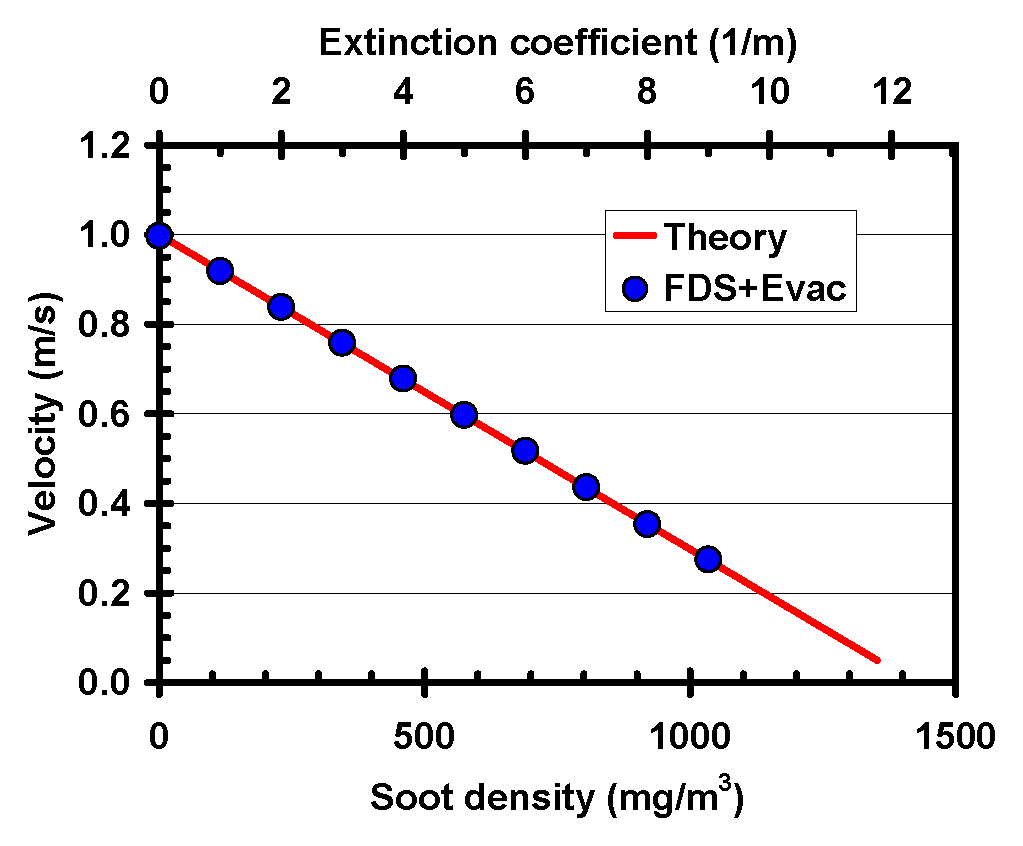
\includegraphics[clip=true,width=80mm]{FIGURES/Smoke_vs_speed}}
  \caption{A smoke vs speed test.}\label{Fig_SmokeSpeedTest}
\end{figure}
%
%
\end{enumerate}
%

\section{Functional Verification}\label{Sec_FuncVeri}

\noindent For the functional verification required by IMO, a good technical
documentation should be enough.  The manual should set out in a
comprehensible manner the complete range of model capabilities and
inherent assumptions and give a guide to the correct use of the
capabilities.  It is left to the reader to decide if this manual
together with the FDS+Evac web pages satisfies this criterion.

\section{Qualitative Verification}\label{Sec_QualVeri}


\noindent The qualitative features of FDS+Evac were tested using some simple
geometries to show that the agents behave like they are told in the
input and that their movement is qualitatively correct.  Most of these
simulations were done in an evacuation trial mode, \emph{i.e.}, there
was no smoke or fire calculation present in the simulations.  The
effect of smoke and toxic gases on the decision making processes of
the agents were tested separately.  An interested reader could
download the input files of the test simulations from the FDS+Evac web
pages and rerun the cases.  This is especially true for some cases,
where the results can not be checked as numbers but one should see
``by own eyes'' that the program is working as it should.

%
\begin{enumerate}
%
\item IMO 8: Counterflow -- two rooms connected via a corridor: Two
  10$\times$10~$\mathrm{m^2}$ rooms are connected with a 10m~long and
  2~m wide corridor.  Initially there are 100 persons in the room 1
  and the room 2 has 0, 10, 50, 100 persons and both rooms move off
  simultaneously.  The expected result is that the time the last
  person from the room 1 enters the room 2 increases as the number of
  persons in counterflow increases.
  
  FDS+Evac results were 41~s and 305~s for the cases, where there were
  0 and 10 persons in the room 2, respectively.  The case, where there
  were 50 persons in the room 2, resulted a very slow movement towards
  the room 2 and the simulation was not run until the end.  If there
  were 100 persons in the room 2 then there were practically no
  movement in the corridor, \emph{i.e.}, a total jam was formed.  This
  is due to the fact that the human density in the corridor is high
  and the default parameters describe agents that are competitive.
%
\item IMO 9: Exit flow -- crowd dissipation from a large public room:
  A 30$\times$20~$\mathrm{m^2}$ public room with four 1.0~m wide exits
  has 1000 persons.  Calculate the time the last person leaves the
  room.  Close two doors and repeat the calculation.  The expected
  result is an approximate doubling of the time to empty the room.
  
  FDS+Evac passed the test.  The total evacuation times calculated
  using the default person properties were 189~s and 361~s when all
  four doors were open and when two doors were closed, respectively.
  These times were 246~s and 455~s when the parameter value
  $\lambda_i$ is changed from the default, which is 0.5, to 0.3.  Note
  that the flows through the 1.0~m doors were below 1.33~p/s when an
  ``Male'' with the parameter value $\lambda_i = 0.3$ is used (1.08
  and 1.13~p/s for the cases all doors open and two doors open,
  respectively).  The default for this parameter is 0.5 and then flows
  through the doors are slightly larger.  See also the door flow test
  case in Sec.~\ref{Sec_CompOtherModels}.
%
\item IMO 10: Exit route allocation: Populate a cabin corridor section
  with 23 persons and allocate the main exit for 15 persons and the
  secondary exit for 8 persons.  The expected result is that the
  allocated passengers move to the appropriate exits.  
  
  FDS+Evac passed the test.  Note that this geometry needed some more
  effort to model, see the FDS+Evac input file on the FDS+Evac web
  pages for more information.  This is due to the fact that in order
  to model the test geometry rigorously the mesh cell sizes for the
  evacuation calculation meshes were 0.1~m in both the $x$ and $y$
  directions.  This is a little bit too fine mesh to construct the
  guiding floor flow fields for evacuation.  This problem does not
  arise if one is modelling the cabinets to have closed doors and
  enters the agents in to the calculation at the cabin doors.
%
\item IMO 11: Staircase: A room populated with 150 persons is
  connected to a 2.0~m wide and 12~m long corridor which ends to a
  2.0~ m wide stairs going upwards.  The expected result is that
  congestion appears at the exit from the room, which produces a
  steady flow in the corridor with the formation of congestion at the
  base of the stairs.
  
  FDS+Evac passed the test, if the user is giving reasonable input
  parameters for the definition of the staircase.  Both models for
  staircases (the \Timtt{\&CORR} and \Timtt{\&EVSS} namelists in the
  input) were used.
%
\begin{figure}[!tb]
  \centerline{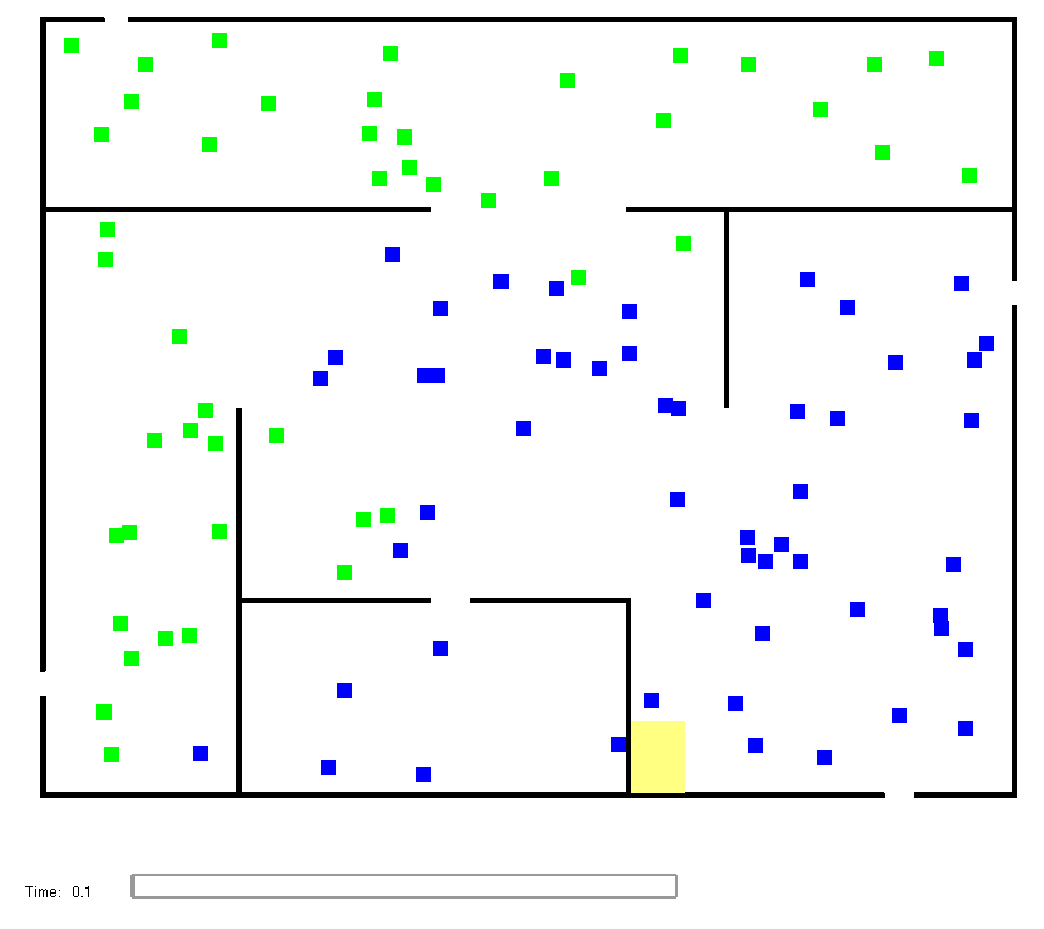
\includegraphics[clip=true,width=60mm]{FIGURES/DoorTestNoSmoke_Doors}
  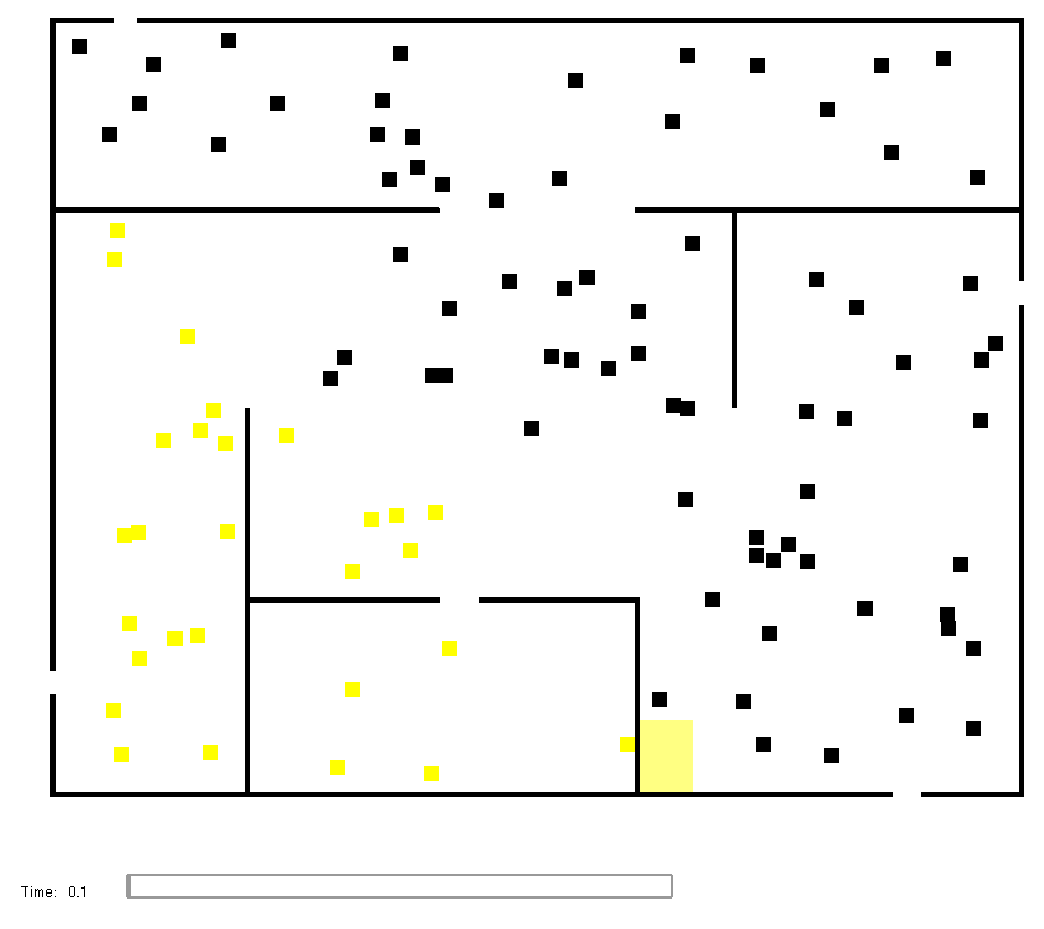
\includegraphics[clip=true,width=60mm]{FIGURES/DoorTestNoSmokeAlgorithm}}
  \caption{An exit door selection test without
    smoke.  On the left, agents are coloured according to their exit
    doors. On the right, they are coloured according to their current
    preference categories.}\label{Fig_ExitDoorNoSmoke}
\end{figure}
%


%
\item Decision making model without smoke: The verification of the
  exit door selection algorithm of FDS+Evac was tested using the
  geometry shown in Figure~\ref{Fig_ExitDoorNoSmoke}.  The figure on the
  left shows the target exit doors for the agents (blue: right bottom
  exit; green: top left exit) and in the figure on the right the
  colours of the agents mark the preference categories of the exit
  door selection algorithm (black: known visible door; yellow: known
  non visible door).  This test case has no smoke and as a result,
  agents use only the known doors (top left and bottom right ones).
  The doors on the left and right walls are not used, because they are
  not defined as ``known doors'' in the input.
  Figure~\ref{Fig_ExitDoorNoSmoke} verifies that the door selection
  algorithm works as intended when there is no smoke.  The agents
  first choose the nearest visible known door, if such exists.  If
  there are no visible doors, the agents choose the nearest non visible
  but known door; see the agents in the bottom left corner of the
  building.  Note however, that in the present version of FDS+Evac,
  the distance to the non visible doors is calculated along a straight
  line through the internal walls.  In later versions, the algorithm
  may be changed to calculate the distance along the streamlines used
  to guide the agents towards the doors.

  
%
\begin{figure}[!b]
  \centerline{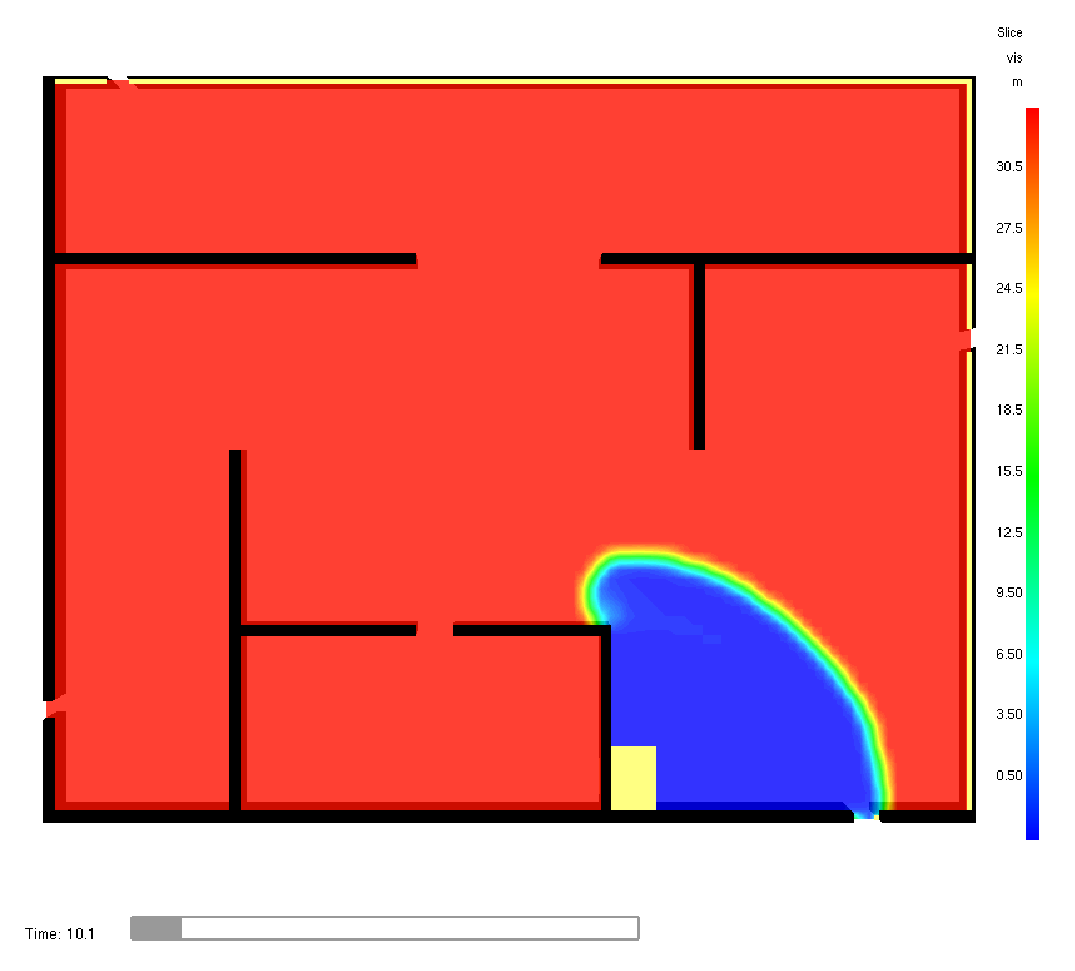
\includegraphics[clip=true,width=80mm]{FIGURES/DoorTestSmokeDens}}
  \caption{The visibility at 10 s in the test case. Red and blue
    colours indicate good and very bad visibilities,
    respectively.}\label{Fig_ExitDoorSmokeDens} 
\end{figure}
%

%
\item Decision making model with smoke: The above test was modified by
  adding a fire that produces smoke to the building.
  Figure~\ref{Fig_ExitDoorSmokeDens} shows the visibility at the
  height of the human eyes at 10~s from the ignition.  The door
  selections and preference categories at the same time are shown in
  Figure~\ref{Fig_ExitDoorSmoke}.  Now the smokiness has changed the
  preferences.  First choices are still the doors with no smoke.  The
  input files for the exit selection tests are on the FDS+Evac web
  page an interested reader is able to rerun the simulations and use
  Smokeview to see that the door selection algorithm is functioning
  like intended.

\begin{figure}[!tb]
  \centerline{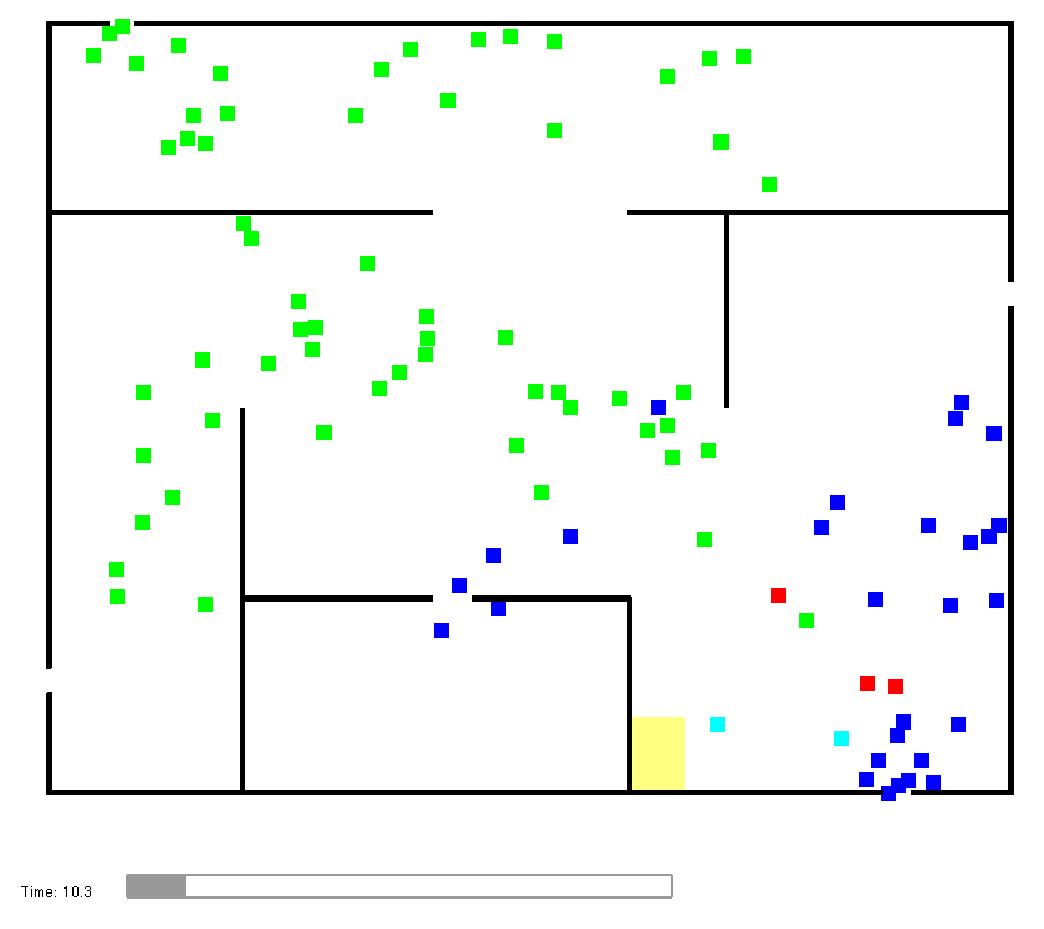
\includegraphics[clip=true,width=60mm]{FIGURES/DoorTestSmoke_Doors}
  x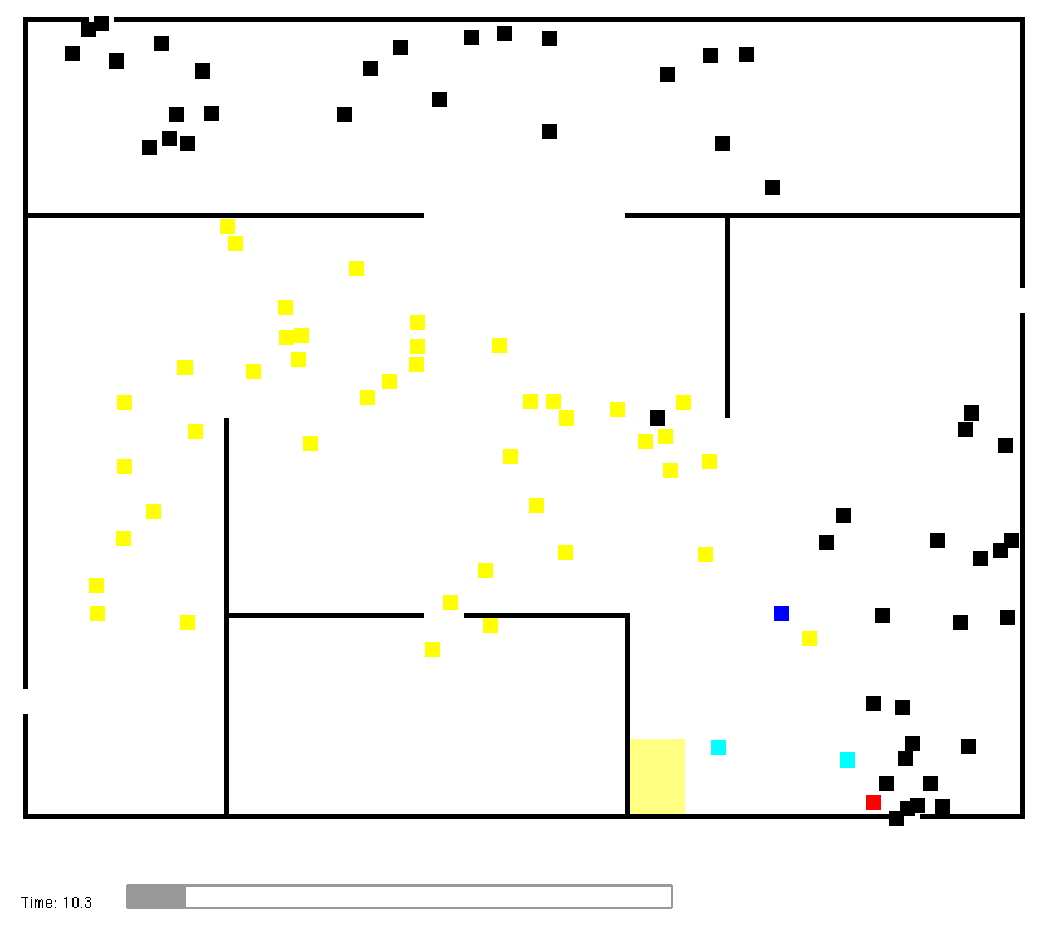
\includegraphics[clip=true,width=60mm]{FIGURES/DoorTestSmokeAlgorithm}}
  \caption{An exit door selection test with
    smoke.  On the left, agents are coloured according to their exit
    doors. On the right, they are coloured according to their current
    preference categories.}\label{Fig_ExitDoorSmoke}
\end{figure}

%
\end{enumerate}
%


\section{Numerical Tests}\label{Sec_NumTest}

\noindent The numerical accuracy of the model depends on the time step used to
solve the equations of motion of the agents.  The time step was chosen
mainly by trial-and-error.  There are some convergence checks made,
see the paper by Korhonen \emph{et al}.~\cite{Korhonen08b}.

\clearpage

\newpage

\chapter{Model Sensitivity}\label{Sec_ModelSensi}

\section{Introduction}

\noindent This section concentrates on the effects of different input parameters
on the FDS+Evac results.  Especially the flows through doors,
corridors and stairs are examined, because these are usually the main
bottlenecks of an evacuation of a building.  This section does not
address the point if the chosen algorithms, numerical methods, etc.
are appropriate for the evacuation simulation or not.  Only the
sensitivity of the chosen algorithms and numerical methods are examined
and reported.  The tests presented here are done in a ``fire drill''
mode, \emph{i.e.}, the egress process is simulated without any fire
calculation.

\section{Numerical Mesh Sensitivity}\label{Sec_GridSensi}

\noindent In principle, the movement algorithm of the agents described in
Sec.~\ref{Sec_BasisModel} does not have any underlying computational
mesh.  The algorithm is continuous in time and space.  But the
implementation of the method in FDS+Evac introduces computational
meshes.  These meshes are used to define the geometry of the
calculation.  The most obvious mesh sensitivity issue is that the
resolution for the obstructions, like doors, stairs, \emph{etc.}, is
the mesh resolution.  The other, subtler effect, is the way how the
mesh resolution changes the evacuation flow fields used to guide
agents to the exit doors.  In some cases, a finer grid does not always
mean a better guiding field for agents.  If the evacuation mesh
resolution is much less than the half of the body dimension then one
may find some difficulties to obtain nice evacuation flow fields, see
the IMO test case 10 in Sec.~\ref{Sec_QualVeri}.

The FDS fire calculation mesh has effects on the evacuation
calculation via the smoke, toxic gas, temperature, and radiation level
calculation.  These quantities are taken to have constant values in
the evacuation mesh cells.  How accurate are the predictions of FDS
for the fire products will, of course, depend on the FDS mesh
resolution.  See the FDS Technical Guide~\cite{FDS_Manual}, and the
verification and validation guides~\cite{FDS_VVGuide1,FDS_VVGuide2}
for the effects of the mesh resolution on the FDS fire calculation.
The evacuation calculation interpolates the fire calculation results
to the 2D evacuation meshes and the evacuation mesh resolution will
have an effect on the spatial accuracy of this fire related
information, but usually grid sizes are equal or less than the
dimensions of a human body and, thus, the accuracy of the fire
information in the evacuation meshes is fine enough for the accuracy
level of the evacuation calculation.  There are many more factors
affecting the calculation of the fire--agent interaction more than the
spatial resolution of the evacuation and fire meshes, \emph{e.g.}, the
production of CO and other toxic gases depend largely on the user
inputs.



\section{Human Parameter Sensitivity}\label{Sec_HumParSensi}

%
\begin{figure}[!tb]
  \centerline{ 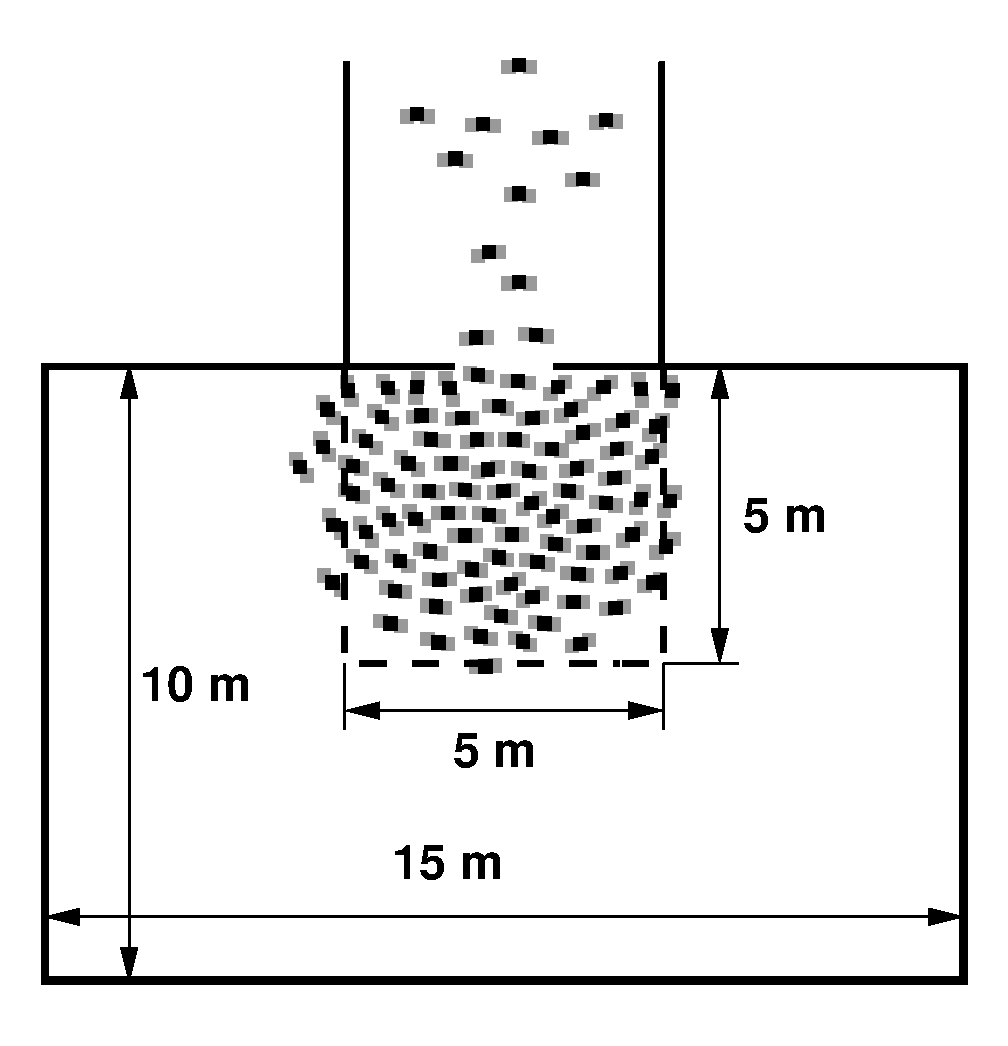
\includegraphics[clip=true,
    width=60mm]{FIGURES/Door_Geom} ~~~~~~~~   
    \includegraphics[clip=true,width=60mm]{FIGURES/CorrGeom2} }
  \caption{Test geometries used to calculate the specific flows through
    doors and corridors.\protect\hspace{200mm}}\label{Fig_Geoms}
\end{figure}
%

\noindent The agent movement algorithm of FDS+Evac has many parameters.  Some of
these are related to the physical description of humans, like the body
size, the mass, the walking speed, and the moment of inertia.  The
others are the parameters of the chosen movement model, $\tau_i$,
$\tau^z_i$, $\omega^0_i$, the parameters of the social force, $A_i$,
$B_i$, $\lambda_i$, and the parameters of the contact force, $k_i$,
$\kappa_i$, $c_d$.  To test the relative importance of these
parameters, Monte Carlo simulations were performed to find the
parameters, which have the greatest effect on specific flows.  The
calculations were done using Evac version 2.0.0, but the basic
movement algorithm has not changed for version 2.1.1, so there is no
need to recalculate these simulations.

Two different geometries were used in the Monte Carlo simulations, see
Figure~\ref{Fig_Geoms}. One of the geometries was used to study the flow
through a narrow door and through a wide door and the other geometry
was used to study flows in a corridor using densities 1.0 and 2.0
persons per square metre.  There were 100 agents randomly located at
the $5 \times 5 ~\mathrm{ \textrm{m}^\textrm{2} } $ square in the door
flow calculations.  Corridor flow calculations had 96 or 192 agents
inside the corridor depending on the density.  Thousand egress
simulation with different random initial properties were performed for
each of these four different cases.  The default ``Adult'' agent type
of FDS+Evac was used in the calculations, but in total eleven model
parameters, $A_i$, $B_i$, $\lambda_i$, $v^0_i$, $\tau_i$, $A_w$,
$B_w$, $\lambda_w$, $\omega^0_i$, $\tau^z_i$, and $I^z_{i}$ were
varied $\pm 20~\%$ about their means using uniform distributions.  The
monitored output quantity was the specific flow in all cases and the
Spearman's rank correlation coefficients (RCC) were calculated for
these four cases and they are shown in Figure~\ref{Fig_RCC}.

%
\begin{figure}[!tb]
  \centerline{ 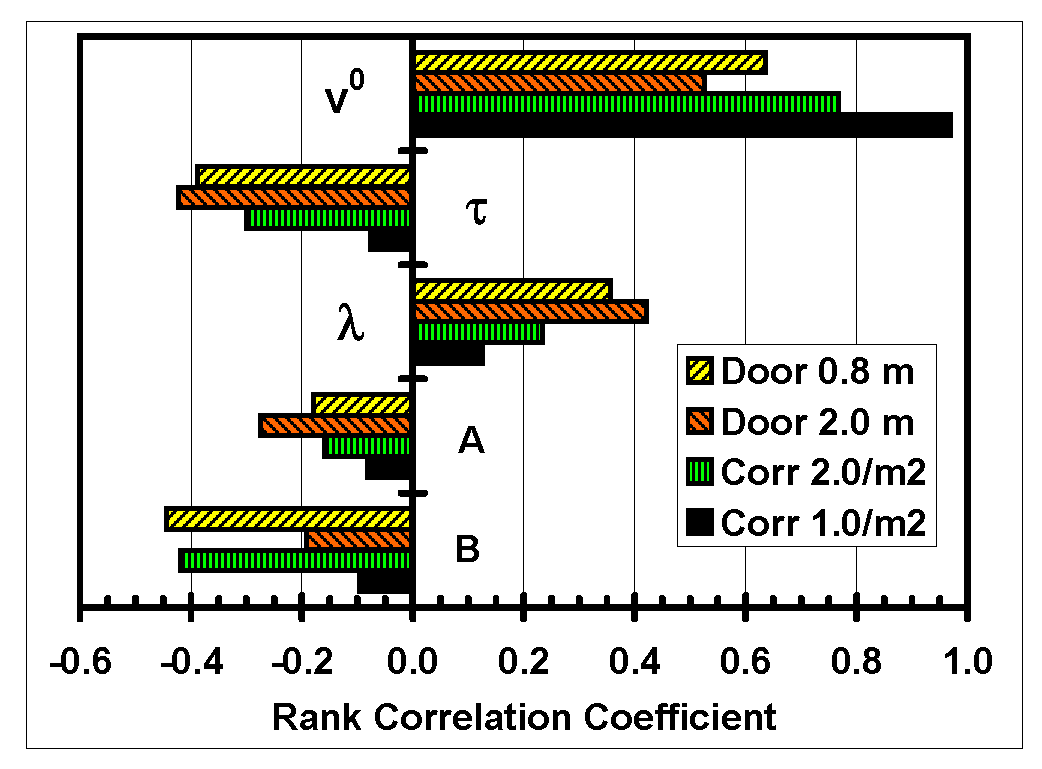
\includegraphics[clip=true, width=75mm]{FIGURES/RCC_DoorCorr_new1} 
               \includegraphics[clip=true, width=75mm]{FIGURES/RCC_DoorCorr_new2} }
  \caption{Rank correlation coefficients (RCC) for specific flows through
    doors and corridors. Widths 0.8~m and 2.0~m were used for doors
    and human densities 1.0~$\mathrm{ \textrm{m}^\textrm{-2} } $ and
    2.0~$\mathrm{ \textrm{m}^\textrm{-2} } $ were used for
    corridors.\protect\hspace{200mm}}\label{Fig_RCC}
\end{figure}
%


It is seen from Figure~\ref{Fig_RCC} that the parameters $A_i$, $B_i$,
$\lambda_i$, $v^0_i$, $\tau_i$, and $B_w$ have the largest impact on
the specific flows through doors and corridors. Thus, further
simulations were done to quantify these effects. Each of these six
parameters were varied separately and 100 simulations were done for
each discretely chosen value of the parameters.  Two different door
widths, 1.0~m and 2.0~m, were chosen to represent a narrow and a wide
door.  Corridor flow was calculated using a density of 2.0 persons per
square metre, because it is known that around this density the
specific flow has its maximum value.  For the density 1.~0 persons per
square metre the corridor flow is mainly specified by the used
distribution for the unimpeded walking speeds, because at this density
the agents can move relatively independently of each others in the
corridor.  The results of these, in total almost 20~000 simulations,
are shown in Figure~\ref{Fig_Door1}, where the markers represent the
average of 100 simulations and standard deviations are shown as error
bars.  Note that in FDS+Evac the initial properties and positions of
the agents are not deterministic, because agents are randomly
positioned, the parameters $R_d$, $v^0$, and $\tau_i$, are sampled
from random distributions and there are small random forces in
Eqs.~\ref{Eq_motion} and \ref{Eq_rotmotion}.  Increasing the values of
$A_i$ and $B_i$ increases the social force which tries to keep agents
apart from each other and, thus, the specific flow for door geometry
will decrease.  The corridor case has a constant agent density.  Thus,
these two parameters can not have an effect through the density.
Larger social force, \emph{i.e.}, larger $A$ and/or $B$, will make a
forward walking person to reduce his/her speed in order not to step on
someone's heels, when the anisotropy parameter, $\lambda_i$, is less
than unity.  Increasing the walking velocity will, of course, increase
the specific flow.  Decreasing $\tau_i$, \emph{i.e.}, increasing the
motive force to go forward, increases specific flows quite rapidly for
the door geometry.  This effect is not as pronounced in the corridor
case, because there is no free space in front of the agents to
accelerate and also the agents are already moving with some velocity
whereas they are almost standing and waiting their turn in front of
the door.  The anisotropy parameter of the social force, $\lambda_i$,
controls how eager agents are to push those who are in front of them.
When $\lambda_i$ is large then agents are 'pushy'.  The effect of the
wall force parameter $B_w$ is to modify the effective width of doors
and corridors, thus, increasing its value will make the effective
width smaller and this will decrease specific flows slightly.

%
\begin{figure}[!tb]
  \centerline{ \includegraphics[clip=true, width=50mm]{FIGURES/DoorCorr_Anew} 
  \includegraphics[clip=true, width=50mm]{FIGURES/DoorCorr_Bnew}
  \includegraphics[clip=true, width=50mm]{FIGURES/DoorCorr_Lambdanew} } 
  \centerline{ \includegraphics[clip=true, width=50mm]{FIGURES/DoorCorr_v0new} 
  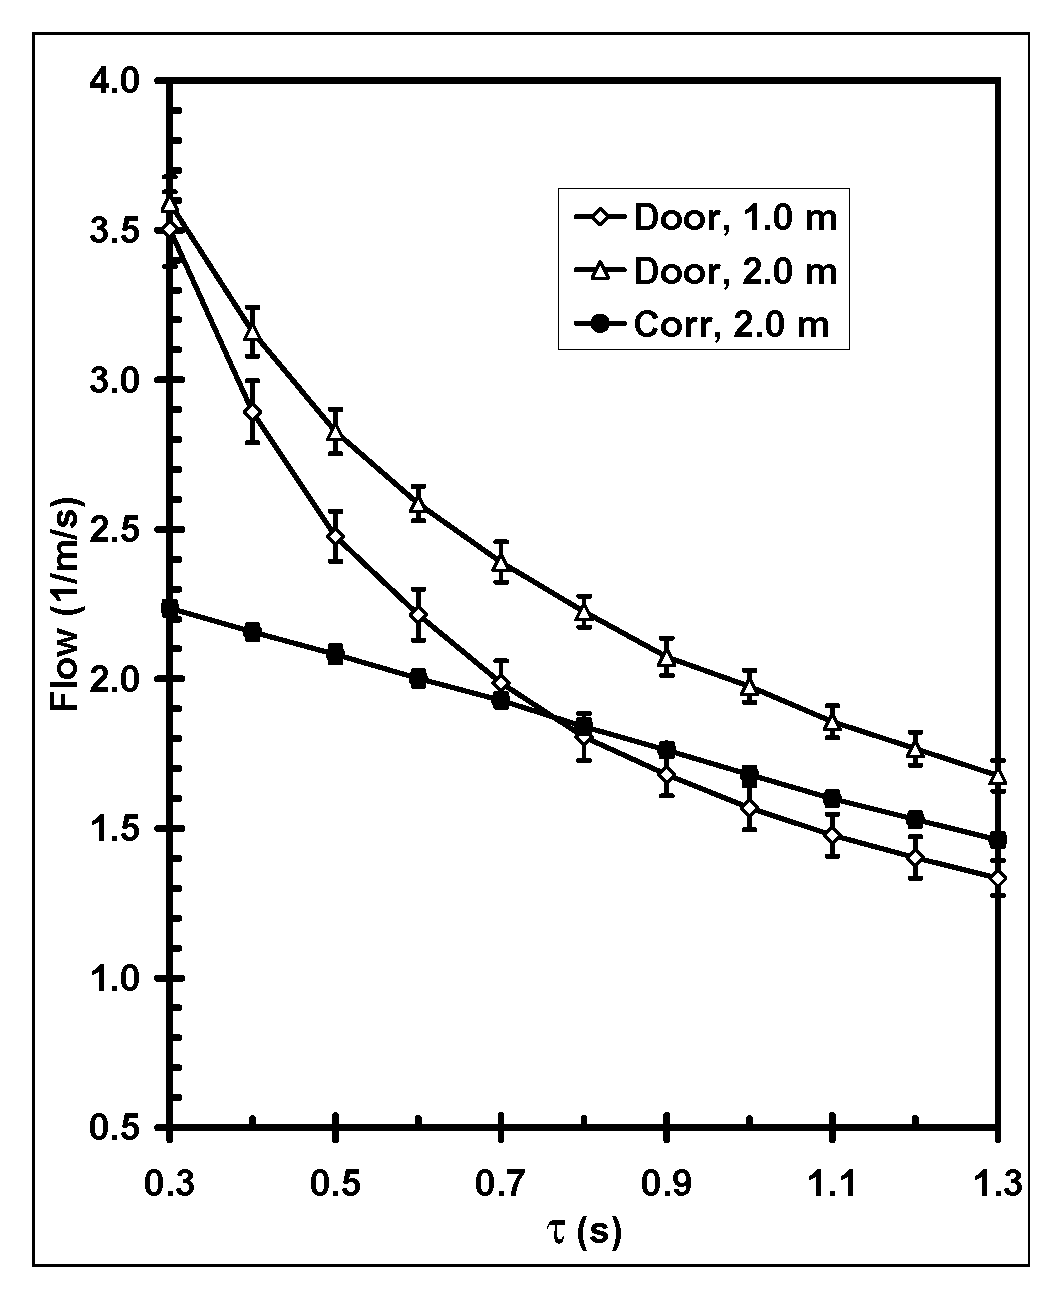
\includegraphics[clip=true, width=50mm]{FIGURES/DoorCorr_Taunew}
  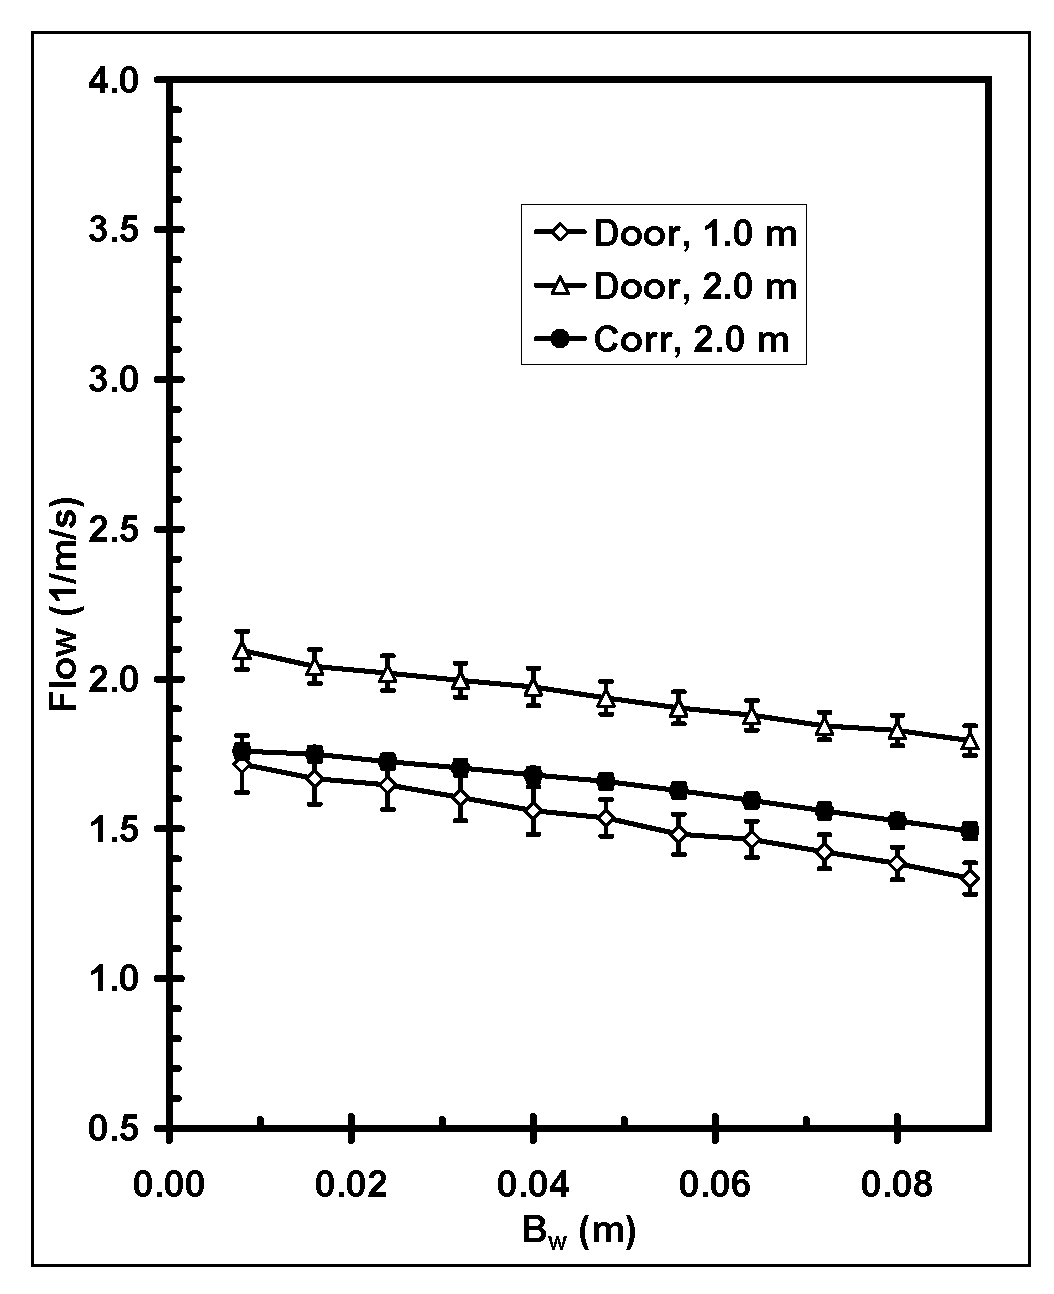
\includegraphics[clip=true, width=50mm]{FIGURES/DoorCorr_Bwallnew} } 
  \caption{Effects of different model parameters, $A_i$, $B_i$,
    $\lambda_i$, $v^0$, $\tau_i$, and $B_w$ on the specific flows
    through doors and corridors.  The corridor is 2.0~m wide, the
    agent density is 2.0~$\mathrm{ \textrm{m}^\textrm{-2} }$, and two
    different doors widths, 1.0~m and 2.0~m, are used.
    \protect\hspace{200mm}}\label{Fig_Door1}
\end{figure}
%

\section{Summary}

\noindent One should be very careful when constructing the geometry, where
agents are moving.  One should use Smokeview to see the guiding flow
fields for the agents before making a full evacuation simulation.  To
see the actual evacuation geometry and the flow fields, one should do
just a plain evacuation calculation without any fire meshes and see
the results in Smokeview.  One should especially check that there are
no smaller than about 0.7~m wide ``holes'' in the evacuation geometry,
because the agents need at least this wide exit paths.

The effect of the parameters in the agent movement algorithm,
Eqs.~\ref{Eq_motion}--\ref{Eq_motive_torque}, are understood well and
user should usually not use any other than the predefined person
types in FDS+Evac.  The default predefined person types use a value
of 0.5 for the anisotropy parameter, $\lambda_i$, of the social force.
For some applications the resulting specific flows may be considered
to be too large.  If this is the case then the user should use 0.3 as
the value of $\lambda_i$.

\clearpage

\newpage

\chapter{Model Validation}\label{Sec_ModelValid}


\section{Introduction}

\noindent Previous chapters are dealing on the fact that how the implementation
of the model worked as a computer code.  \emph{I.e.} it was tested
that the programme is functioning as planned and it was also considered
how sensitive the model is to its input parameters.  These tests give
confidence on how the model is working and how accurate the model
equations are solved numerically.  But these tests do not necessary
tell how well the model is modelling the actual evacuation scenarios.
For this reason, in this chapter the model predictions are tested
against experimental data from evacuation experiments and trial
evacuations.  The model predictions are also compared to other
evacuation models.



\section{Comparisons with Test Data}

\noindent This chapter lists three test cases, where the FDS+Evac predictions
are compared to experimental data on human flows on horizontal paths
and stairs.  These calculations were done using Evac version 2.0.0,
but the basic movement algorithm has not changed for version 2.1.1, so
there is no need to recalculate these simulations.

%
\begin{enumerate}
%
\item Specific flows through corridors: In the research of pedestrian
  flows, the dependence of the specific human flow rate on the human
  density is called as ``fundamental diagram''.  It shows how the
  specific flow first increases when the human density is increased,
  but then starts to decay as the density becomes high enough to
  hinder the walking.  In this test case, the specific flow rates
  given by the FDS+Evac code are compared to experimental walking
  velocities on horizontal floors in corridor geometry.  The geometry
  is shown in Figure~\ref{Fig_Geoms}.  The corridor is modelled as a
  loop to avoid the effects of inflow and outflow boundary conditions.
  In Figure~\ref{Fig_CorrResults}, the predicted flow rates are
  compared against some experimental results for pedestrian traffic
  flows taken from Daamen's thesis~\cite{Daamen04}.  Note that almost
  all of the experimental information is obtained by studying
  bidirectional pedestrian flows, the results for unidirectional flows
  might give different results.  The FDS+Evac simulations were
  performed with two different parameter sets, labels ``1'' refer to
  the defaults of FDS+Evac and labels ``2'' refer to parameter sets,
  where $\lambda_i = 0.3$ is used.


%
\begin{figure}[!tb]
  \centerline{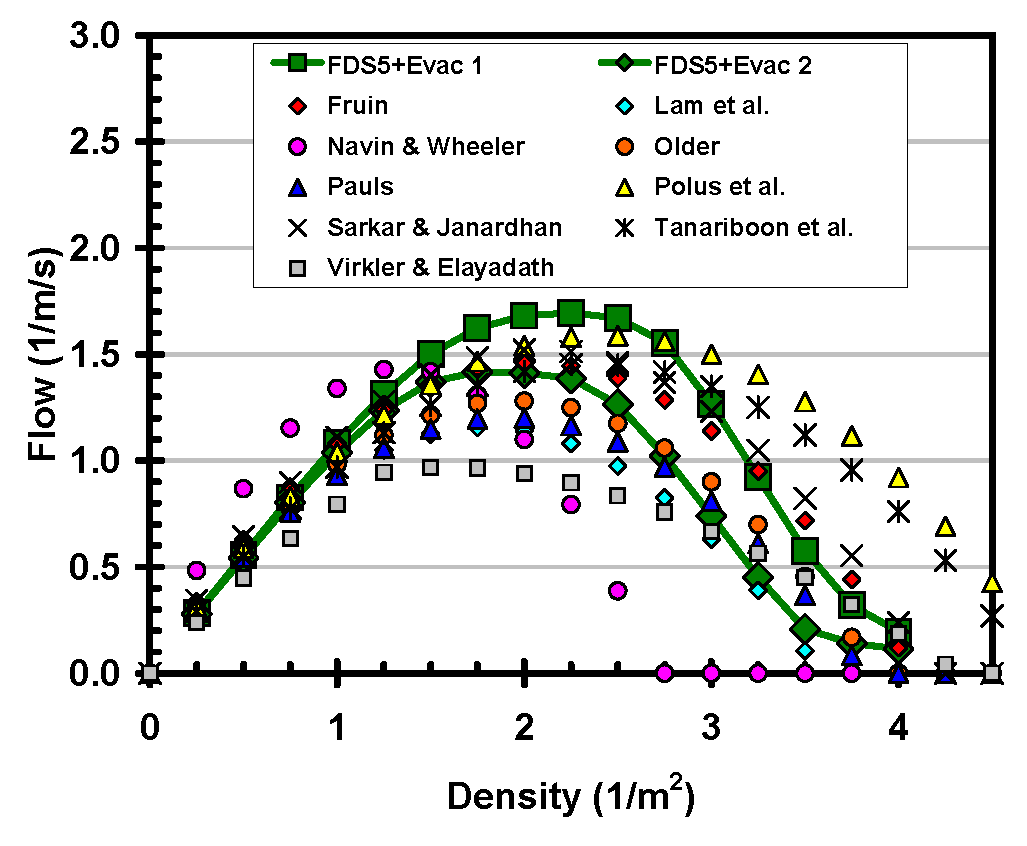
\includegraphics[clip=true,width=80mm]{FIGURES/CorrFlowResults}}
  \caption{The specific flows in corridors.}\label{Fig_CorrResults} 
\end{figure}
%



%
\begin{figure}[!b]
  \centerline{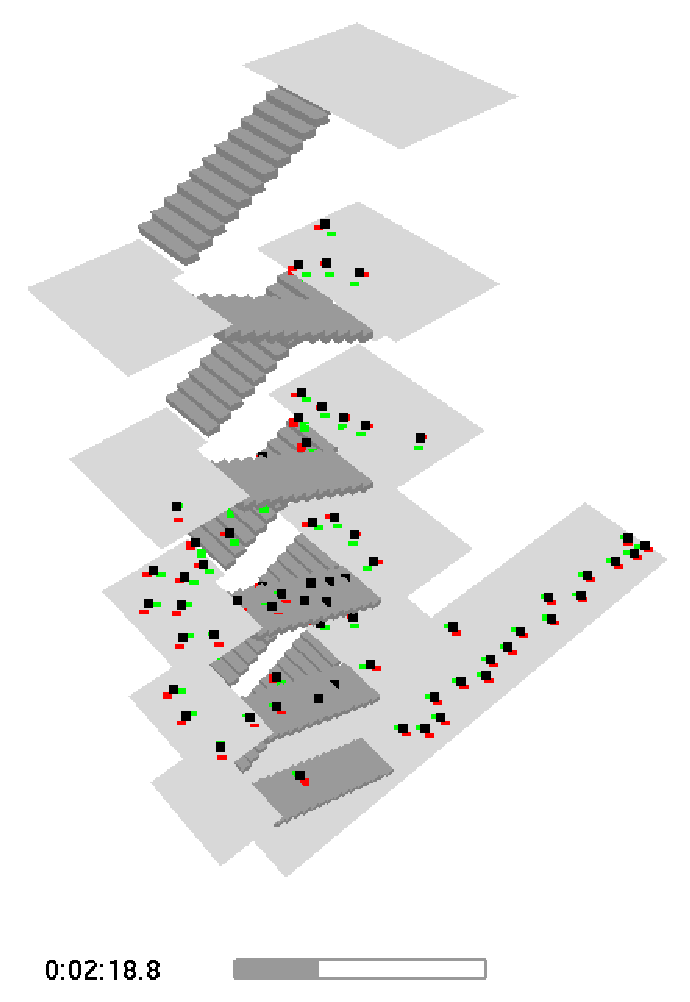
\includegraphics[clip=true,width=60mm]{FIGURES/PorrasKuva}}
  \caption{A snapshot from a FDS+Evac simulation showing the geometry
  of the staircase.}\label{Fig_StairGeom} 
\end{figure}
%

%
\item Staircase of an office building: The evacuation experiment at
  the large office building~\cite{Hostikka07b} was modelled using
  FDS+Evac.  Since the experiment was strongly focused on just one
  staircase, only this staircase was modelled.
  Figure~\ref{Fig_StairGeom} shows the geometry of the studied
  staircase.  The actual dimensions and door positions can be found in
  the experimental report~\cite{Hostikka07b}.  The experimental
  entry times of humans to the stair landings were taken as inputs to
  the simulations.  The standard adult person type of FDS+Evac was
  used in the simulations.  Two different values were used for the
  anisotropy parameter of the social force, $\lambda_i=0.5$ which is
  the default, and $\lambda_i=0.3$ which corresponds to more relaxed
  egress.  The calculations for staircases were performed using both
  models for staircases available in FDS+Evac.
  

%
\begin{figure}[!tb]
  \centerline{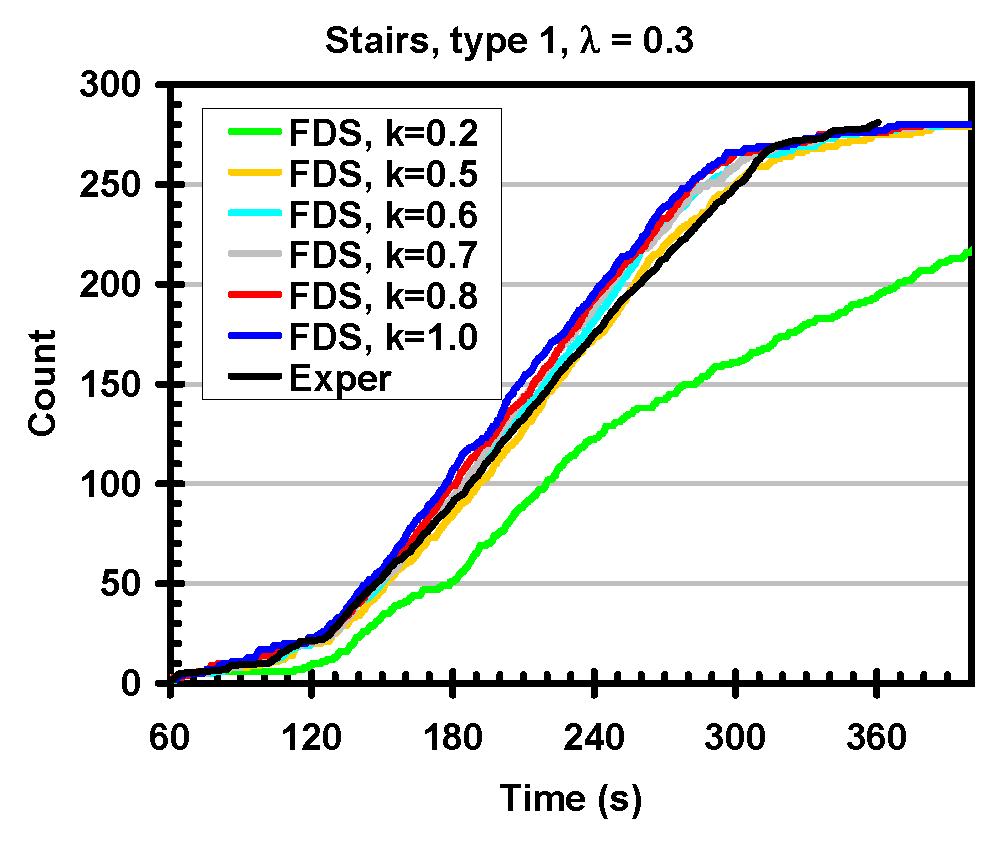
\includegraphics[clip=true,width=60mm]{FIGURES/StairsType1Lam0p3}
  \includegraphics[clip=true,width=60mm]{FIGURES/StairsType1Lam0p5}}
  \caption{Comparison of FDS+Evac (staircase model type 1) and experimental
    observations of a staircase flow.  Values 0.3 (left) and 0.5
    (right) for the anisotropy parameter of the social force are used.
    Different curves correspond to the different values of the
    staircase speed reduction parameter $k$.}\label{Fig_StairType1}
\end{figure}
%

%
\begin{figure}[!b]
  \centerline{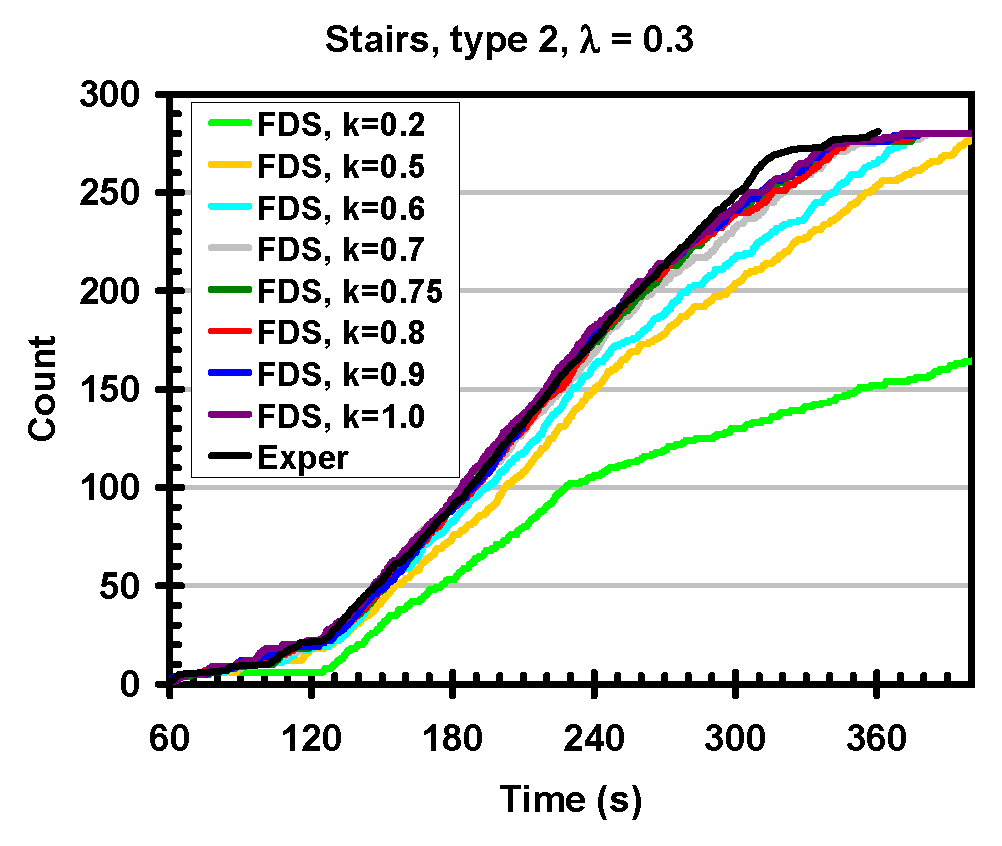
\includegraphics[clip=true,width=60mm]{FIGURES/StairsType2Lam0p3}
  \includegraphics[clip=true,width=60mm]{FIGURES/StairsType2Lam0p5}}
  \caption{Comparison of FDS+Evac (staircase model type 2) and experimental
    observations of a staircase flow.  Values 0.3 (left) and 0.5
    (right) for the anisotropy parameter of the social force are used.
    Different curves correspond to the different values of the
    staircase speed reduction parameter $k$.}\label{Fig_StairType2}
\end{figure}

  Figure~\ref{Fig_StairType1} shows a comparison of the experimental
  observations and the simulation results using the simple staircase
  model (type 1).  This model is implemented using the \Timtt{CORR}
  namelist, which is a crude model for stairs.  In each figure,
  several simulated curves are shown corresponding to different values
  of the staircase speed reduction parameter.  In
  Figure~\ref{Fig_StairType1}, the best results are obtained when the
  value for the speed reduction parameter is 0.5, \emph{i.e.}, the
  movement speeds of the agents are reduced to $v = 0.5v_0$ at the
  stairs.  The results using more sophisticated way of defining
  staircases (type 2) are compared to the observed values in
  Figure~\ref{Fig_StairType2}.  In these simulations, the stairs are
  modelled as inclines (\Timtt{EVSS} namelist), where agents move at
  reduced speed.  Reducing the walking speed by a factor ~0.7 gives a
  good agreement with the observations.  Whether the anisotropy
  parameter $\lambda_i$ is 0.3 or 0.5 does not have effect of any
  practical importance.
%
%


\begin{figure}[!tb]
  \centerline{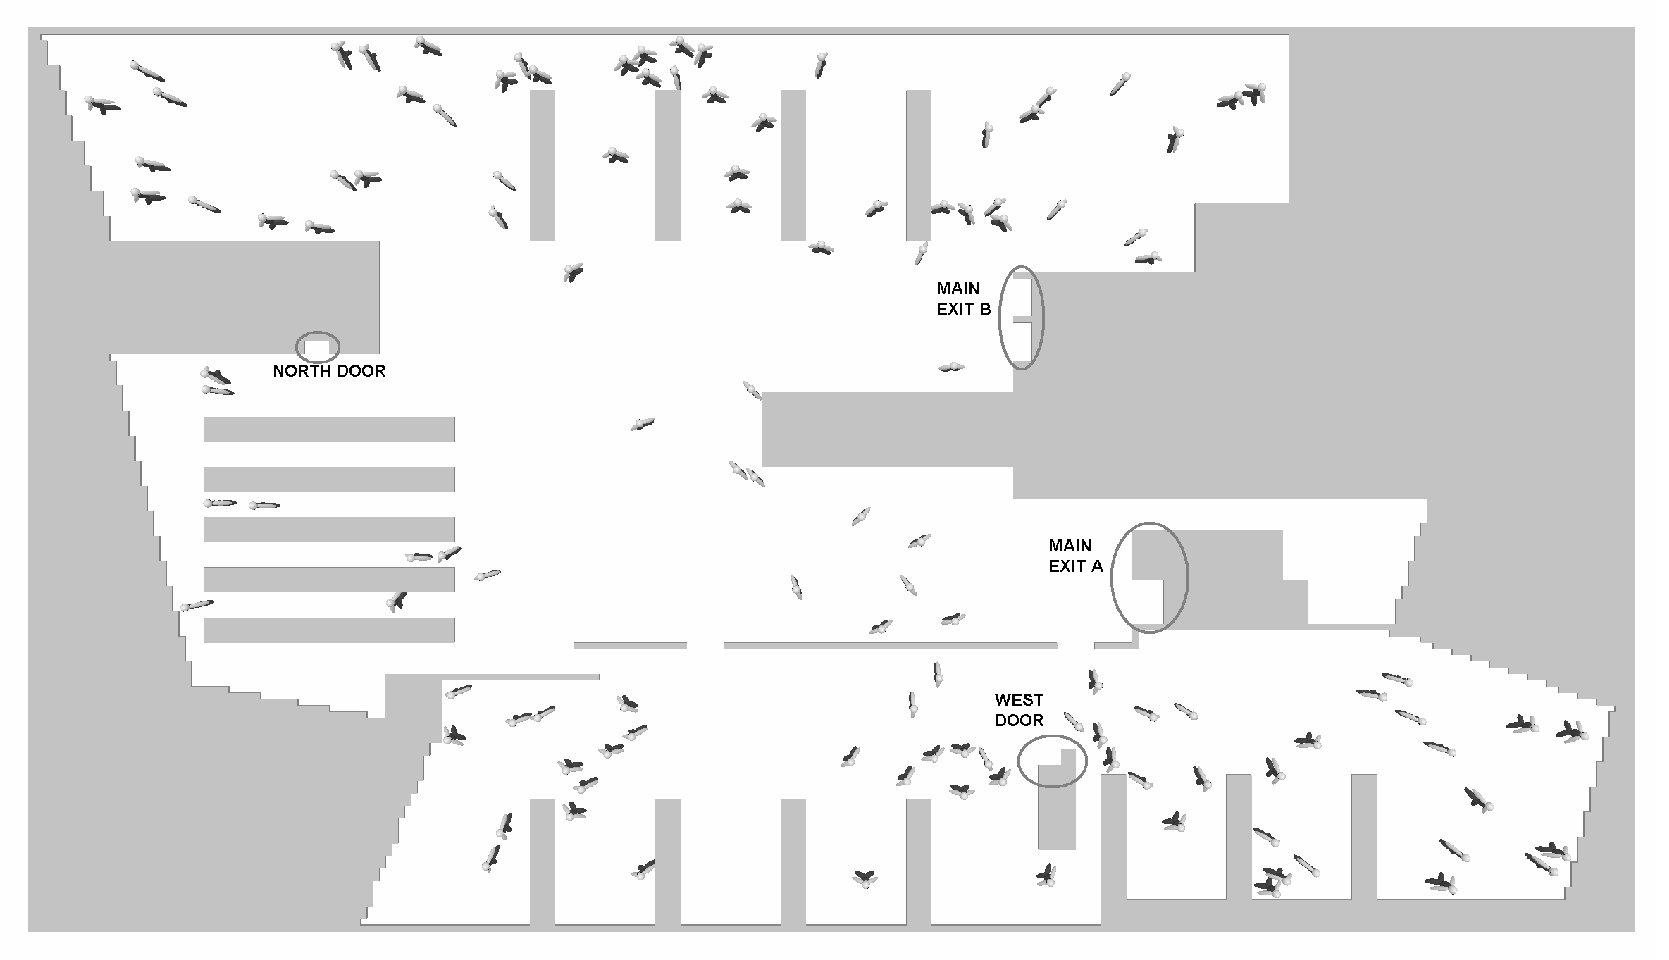
\includegraphics[clip=true,width=120mm]{FIGURES/Library_Kuva2}}
  \caption{A snapshot from a FDS+Evac simulation shows the geometry of the
    FDS+Evac model for the second floor of the public
    library.}\label{Fig_Kirjasto}
\end{figure}

%
\item Public library: An observed evacuation experiment of a public
  library~\cite{Hostikka07b} was simulated to study the capability to
  predict the entire movement phase of the evacuation, consisting of
  movement inside the floor, queueing to the staircase and finally
  movement through a narrow staircase to the exit.  The simulation
  geometry and the initial positions of the persons are shown in
  Figure~\ref{Fig_Kirjasto}.  As the majority of persons in the building
  used the north exit door, the main results are for this door.  Shown
  are also the results for the west door, where about 50\% of the
  people originated from the first floor.  In the simulations, only
  the second floor of the building was simulated and people
  originating from the first floor were placed into the second floor.
  The north door was the only door with observed crowding.

%
\begin{figure}[!tb]
  \centerline{\includegraphics[clip=true,width=80mm]{FIGURES/KirjastoTulokset}}
  \caption{Comparison of FDS+Evac simulation results and observations
    at the north and west doors of the public
    library.}\label{Fig_KirjastoResults} 
\end{figure}
  
The decision making processes were not modelled.  Instead, the people
were allocated for the north and west doors according to the ratio
observed in the experiment.  The simulations were performed using the
standard agent type ``Adult''.  The pre-movement times were generated
from symmetric triangular distribution with mean of 41~s and lower and
upper limits of 11~s and 71~s, respectively.  A comparison of the
simulated and experimentally observed flows is shown in
Figure~\ref{Fig_KirjastoResults}.  As can be seen, the predicted flow
rates are in very good agreement with the experiments.  For the west
door, the results reflect the goodness or badness of the assumed
pre-movement time distribution because the flow rate through the door
is so small.  For the north door, the simulation is very relevant,
because the flow rate is mainly determined by the geometry and the
crowd dynamics during the queueing process.
%
%
\end{enumerate}
%

%Case 1: RI Nightclub: ToDo

%Case 2: Theatre at Tampere, Finland: ToDo

%Case 3: Stairs in an office building in Helsinki.

% ToDo: stair flows vs correlations

\section{Comparisons with Other Evacuation Models}\label{Sec_CompOtherModels}

\noindent The FDS+Evac model is compared here to other evacuation models using
four different geometries.  The FDS+Evac results and corresponding
input files are on the FDS+Evac web pages and some of these cases are
also discussed in the summary report of the FDS+Evac development
project~\cite{Hostikka07a}.  These calculations were done using Evac
version 2.1.0, but the basic movement algorithm has not changed for
version 2.1.1, so there is no need to recalculate these simulations.
%



%
\begin{figure}[!b]
  \centerline{\includegraphics[clip=true,width=80mm]{FIGURES/SportHallGeom}}
  \caption{The geometry of the studied sports hall.  The open grey
    area shows, where the agents are at the start of the simulations.
    The red rectangle shows the fire location, which is close to door
    3 and, thus, this door is not used.}\label{Fig_SportGeom}
\end{figure}
%

\begin{enumerate}
%
\item Sports hall: FDS+Evac simulations were compared to
  Simulex~\cite{Simulex96, Thompson95a, Thompson95b, Thompson03}
  simulations in a sports hall shown in Figure~\ref{Fig_SportGeom}.  The
  hall was previously analysed by Paloposki \emph{et
    al.}~\cite{Paloposki02}.  The sports hall is used to practice
  different kind of sports.  There are no spectator stands in the hall
  and neither are there any social spaces like showers.  People enter
  the hall through the main entrance (``Door 1''), which is 1.8~m
  wide.  Doors 2 and 3 are 4.0~m wide two leaf doors and doors 4 and 5
  are 0.9~m wide single leaf doors.  It is assumed that a fire starts
  close to door 3 (the shaded rectangle in Figure~\ref{Fig_SportGeom})
  so that this door cannot be used for egress.  235 persons use the
  closest door (``Door 5''), 130 persons use the main entrance (``Door
  1''), 60 persons door 2, and 75 persons use door 4.  Persons are
  initially located at the east end of the hall in an area of
  20$\times$25~$\mathrm{m^2}$ (the open rectangle in
  Figure~\ref{Fig_SportGeom}).  Three different reaction time scenarios
  were considered, two having a normal distribution with a standard
  deviation of 15~s but different means (60~s and 180~s), and one
  having a log-normal distribution (median 75~s, standard deviation of
  the logarithm of reaction time was 0.7).  Actually, the log-normal
  distribution was approximated by two uniform distributions, because
  the version of the Simulex, which was used, did not support
  log-normal distributions for the reaction time.

%
\begin{figure}[!tb]
  \centerline{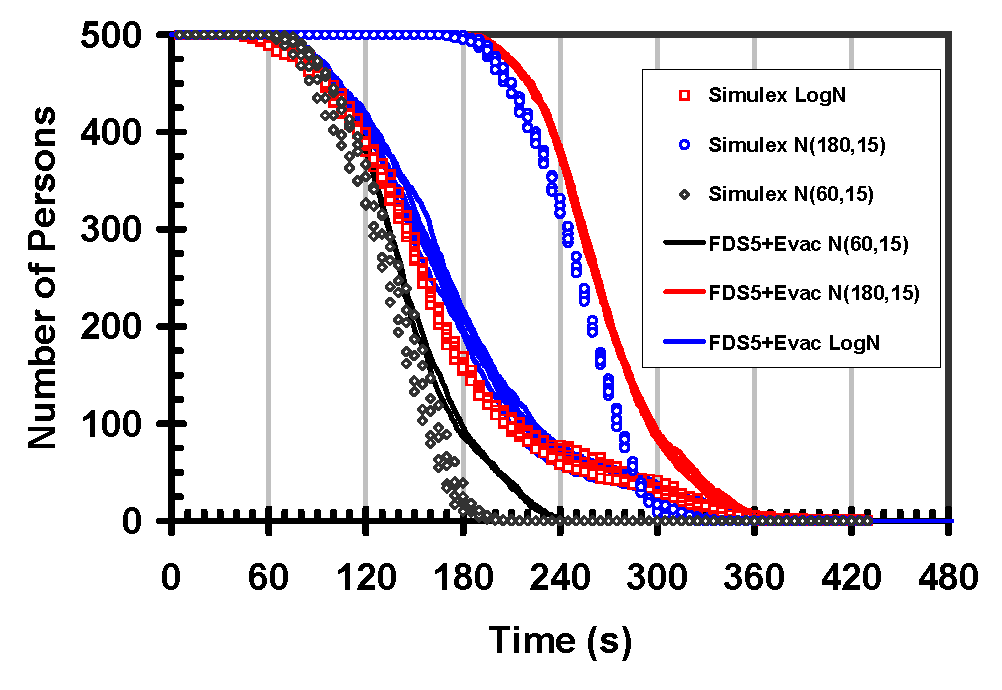
\includegraphics[clip=true,width=80mm]{FIGURES/EerikkilaResults}}
  \caption{The comparison of FDS+Evac to Simulex in a sport hall
    case.  Results of five different simulations are shown for each
    case.}\label{Fig_SportResults}
\end{figure}
%

  
  The results of the simulations are shown in
  Figure~\ref{Fig_SportResults}.  Since both FDS+Evac and Simulex are
  modelling human egress as a stochastic process, the presented
  results were collected from five different runs per case.  The
  FDS+Evac and Simulex results agree very well for the log-normal
  reaction time case, but for the other two cases the results differ
  somewhat.  These differences arise due to the ``Door 5'', which is
  only 1.0~m wide in the FDS+Evac simulations, but through which 235
  persons escape.  The flow through this door is larger in Simulex
  than in FDS+Evac.  The flow through this door in the FDS+Evac
  simulations is 1.55~p/s for the cases, where normal distributions
  were used for the reaction times.  If a value of 0.3 is used for the
  anisotropy parameter $\lambda_i$ the flow is reduced to 1.1~p/s.
  The other doors are not as crowded and there the capacities of the
  doors do not show up as much.
%

%
\begin{figure}[!tb]
  \centerline{\includegraphics[clip=true,width=80mm]{FIGURES/OpenFloorGeom}}
  \caption{The geometry of the open floor office test
    case.}\label{Fig_OpenFloorGeom}
\end{figure}
%

%
\begin{figure}[!b]
  \centerline{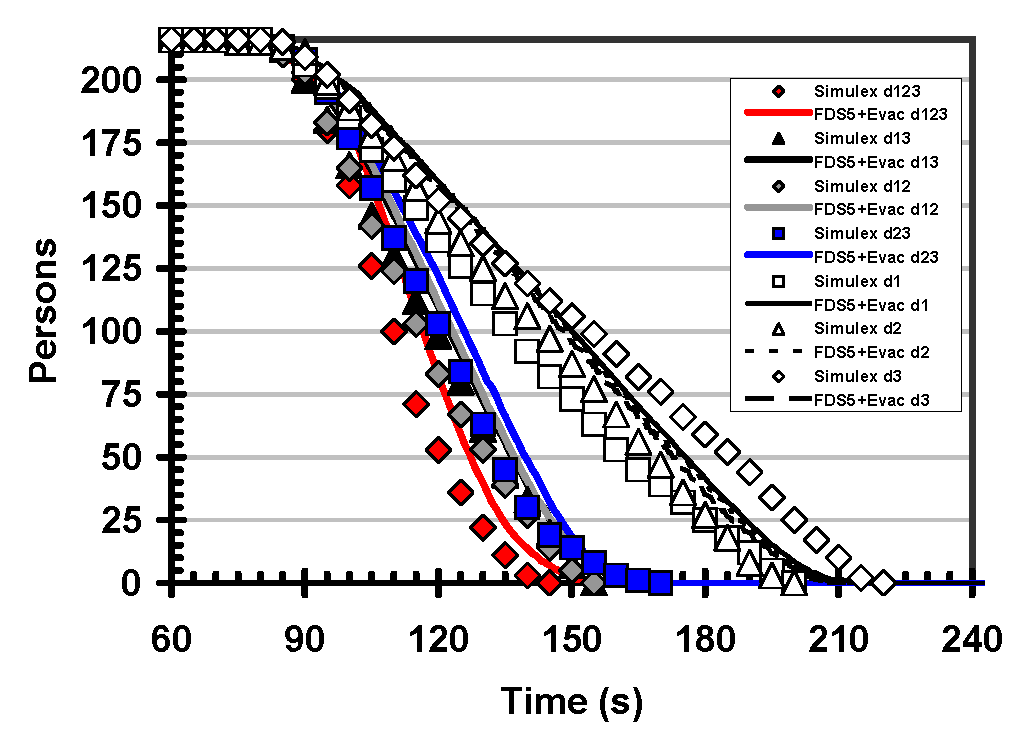
\includegraphics[clip=true,width=80mm]{FIGURES/PankkiTulokset}}
  \caption{The comparison of FDS+Evac to Simulex in an open floor
    office case.}\label{Fig_OpenFloorResults} 
\end{figure}
%

\item Open floor office: This test geometry was an open floor office,
  whose floor plan is shown in Figure~\ref{Fig_OpenFloorGeom}.  The
  floor has dimensions of 40$\times$40~$\mathrm{m^2}$ and there are
  initially 216 persons on this floor.  The properties of these agents
  were assumed to be as the ``Office Staff'' category in the Simulex
  model and the reaction times of the agents were assumed to follow a
  normal distribution with mean of 90~s and standard deviation of
  11~s.  There are three stairs located at the central core of the
  building.  The widths of the doors opening to the stairs are 1.2~m.
  In total seven different egress scenarios were simulated, covering
  the cases where all stairs are in use, one stair is blocked and a
  case where two stairs are blocked.
  
  The results of FDS+Evac simulations are compared to results of
  Simulex simulations in Figure~\ref{Fig_OpenFloorResults}.  Only when
  two exit doors were blocked, queues were formed at the door.  For
  two or three operational doors the main form of the evacuation
  curves arise from the reaction time distribution.  The FDS+Evac and
  Simulex results are quite similar.  It should be mentioned, that in
  the FDS+Evac simulations, the initial (random) positions of agents
  do not change between different door scenarios (see
  Figure~\ref{Fig_OpenFloorGeom}), whereas in Simulex runs the random
  initial positions are different in each calculation.  This explains
  why the Simulex results have larger scatter in the cases where a
  certain number of doors are operational.\vspace{\fill}



%
\begin{figure}[!tb]
  \centerline{\includegraphics[clip=true,width=130mm]{FIGURES/AssemblySpaceGeom}}
  \centerline{\includegraphics[clip=true,width=120mm]{FIGURES/AssemblySpace_Simulex_60s}}
  \caption{A snapshot from (a) FDS+Evac, (b) Simulex
    calculation.}\label{Fig_AssemblySnapshots} 
\end{figure}
%

\pagebreak[3]
%
\item Assembly space: The second test case is a large fictitious
  assembly space having dimensions of 50$\times$60~$\mathrm{m^2}$ and
  1000 people initially inside.  There is only one 7.2~m wide corridor
  leading to the exit.  The geometry is shown in
  Figure~\ref{Fig_AssemblySnapshots}a.  The FDS+Evac results (``Evac'')
  are compared to those of Simulex (``Simulex'') and
  buildingExodus~\cite{Exodus3} (``Exodus'') in
  Figure~\ref{Fig_AssemblyResults}.  Note, that the FDS+Evac simulations
  were also done using parameters describing more relaxed egress
  (labels ``Evac 2''), where the value of the anisotropy
  parameter of the social force, $\lambda_i$, had a value of 0.3
  instead of the default 0.5.
  
  Considerable differences are shown between the results of FDS+Evac
  and the results of Simulex and buildingExodus programmes.  These
  differences can be traced back to the motion of the agents in the
  corridor, see Figure~\ref{Fig_AssemblySnapshots}.  Simulex and
  buildingExodus are not using the whole width of the corridor
  efficiently, when the simulations are done using the default values
  and standard input.  (An advanced user of these codes might be able
  to get different results by using some additional features.)  The
  results of FDS+Evac model look more realistic.
  
  In Figure~\ref{Fig_AssemblyResults} also shown are the results of
  the simulations for a case, where there is no corridor at all,
  \emph{i.e.}, there is just one 7.2~m wide exit door located at the
  wall of the room.  In this case, the agreement between the different
  evacuation programmes is much better.  The calculated specific flows
  (1/p/m) are: Simulex 1.48, Exodus 1.95, FDS+Evac 2.15
  ($\lambda_i=0.5$), and 1.73 ($\lambda_i=0.3$).

%
\begin{figure}[!tb]
  \centerline{\includegraphics[clip=true,width=80mm]{FIGURES/AssemblySpaceResults}}
  \caption{The comparison of FDS+Evac to buildingExodus
    and Simulex in an assembly space.}\label{Fig_AssemblyResults}
\end{figure}
%
%
%
\begin{figure}[!b]
  \centerline{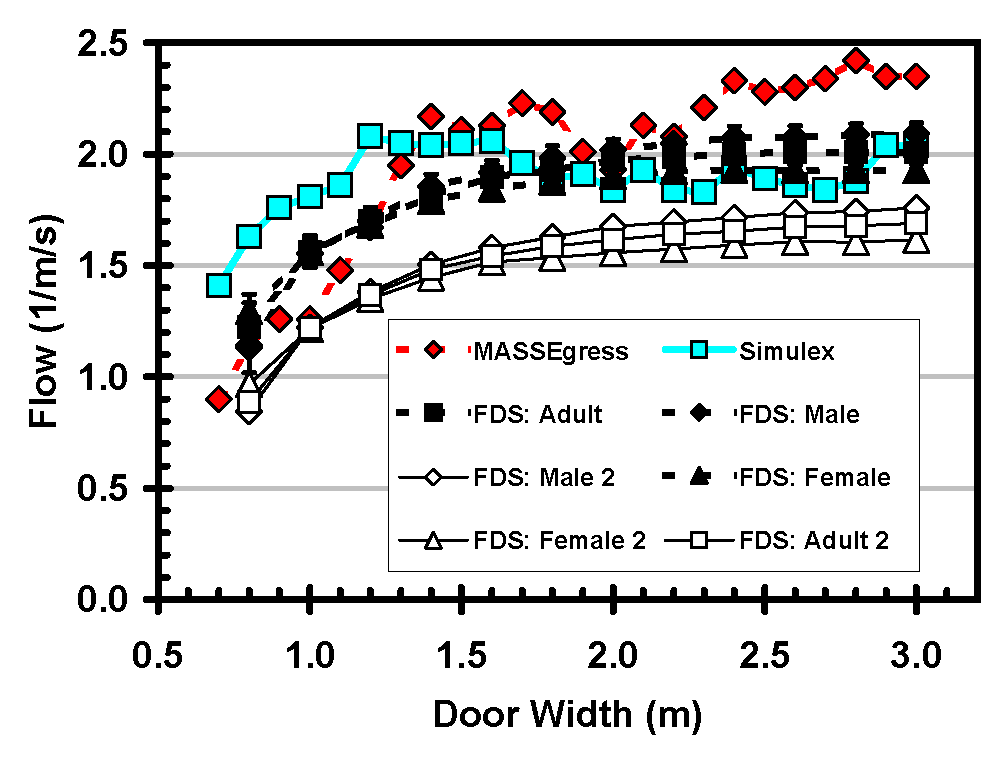
\includegraphics[clip=true,width=80mm]{FIGURES/OviFlowRersults}}
  \caption{The specific flows through doors.}\label{Fig_DoorResults}  
\end{figure}
%

%
\item Specific flows through doors: The fourth test geometry is the
  same as used in Section~\ref{Sec_HumParSensi} for human parameter
  sensitivity studies and it is shown on the left hand side in
  Figure~\ref{Fig_Geoms}.  This geometry is commonly used in the
  literature to calculate the specific flows through doors.  In the
  test, there are 100 agents randomly located at the
  5$\times$5~$\mathrm{m^2}$ square.  In Figure~\ref{Fig_DoorResults},
  the results of FDS+Evac simulations for specific flows through doors
  are compared to simulation programmes Simulex and
  MASSEgress~\cite{Pan06}.  The results of the programmes MASSEgress
  and Simulex are extracted from Pan's thesis~\cite{Pan06}.  The
  FDS+Evac simulations are performed with two different parameter
  sets, labels ``Male''/``Female''/``Adult'' refer to the
  corresponding default agent types of FDS+Evac and labels ``Male
  2''/``Female 2''/``Adult 2'' refer to parameter sets, where
  $\lambda_i = 0.3$ is used.  It is seen that FDS+Evac is able to
  produce reasonable flows through doors.  For some applications, the
  flows generated by the default parameter values may be considered
  too large, but it is quite straightforward to modify the parameters
  of FDS+Evac to reach specific flows that are more relevant to a more
  relaxed egress.

%
\end{enumerate}
%

\clearpage

\newpage


\chapter{Running FDS+Evac}\label{Sec_Running}

\noindent Running FDS+Evac is similar to running FDS, \emph{i.e.}, relatively
simple.  All of the parameters that describe a given fire and egress
scenario are typed into a text file that will be referred to as the
``fds'' or the ``input'' file.  In this document, the data file will
be designated as \Timtt{CHID.fds}.  In practice, the user should
choose the input string \Timtt{CHID} on the \Timtt{HEAD} namelist
group to be the same as in the file name so that all of the files
associated with a given calculation will have a common prefix.

In Chapter~\ref{Sec_SampleFile}, example input files will be
presented.  Several other example files exist at the FDS+Evac web site
\verb+http://www.vtt.fi/fdsevac+.  It is suggested that a new user
starts with an existing input file, runs it as is, and then makes the
appropriate changes to the input file for the desired scenario.  By
running a sample case, the user will become familiar with the
procedure, learn how to examine the results, and ensure that her/his
computer is up to the task before embarking on learning how to create
new input files.

If the user wants to do a combined fire and evacuation simulation,
she/he should first learn how to do fire simulations using FDS.  If
the user is not experienced on doing FDS fire simulations, it is
suggested that the user uses FDS+Evac just to simulate ``fire
drills'', \emph{i.e.}, simulate only the egress part of the problem.
Even in this case the user should read carefully the User's Guide of
FDS~\cite{FDS_UserGuide}, because the evacuation simulation geometry is
constructed similarly as the fire simulation geometry.


\section{Starting a FDS+Evac Calculation} 

\noindent A FDS+Evac simulation is run similarly as a FDS fire simulation, so
read the User's Guide of FDS~\cite{FDS_UserGuide}, where you can find
information on how to run the fire simulation and see the results by
using Smokeview~\cite{SV_UserGuide}.  Below is a short description how
to run FDS+Evac on MS Windows.

Assuming that an input file called \Timtt{CHID.fds} exists in some
directory, the user must run the program in a DOS command shell as
follows:\\ 
Open up a Command Prompt window, and change directories to where the
input file for the case is, then run the code by typing
\begin{verbatim}
    fds5.exe CHID.fds
\end{verbatim}
to begin a run, which will output some text on the Command Prompt
window.  If the user wants to save the text output going on the
Command Prompt window, she/he should type
\begin{verbatim}
    fds5.exe CHID.fds 2&>1 > CHID.err
\end{verbatim}
to begin a run.

FDS+Evac can also be run using the multiple processor version of the
programme (\texttt{fds5\_mpi.exe}).  You should first learn how to run
parallel fire calculations by reading the User's Guide of FDS.  The
combined fire and evacuation simulation can be run almost similarly,
but you should be sure that all fire mesh definitions are preceding
all evacuation mesh definitions, because all the evacuation meshes are
treated as a single thread, \emph{i.e.,} all evacuation meshes are
assigned to same process number.  For example, if you are using MPIH2,
the example \Timtt{config.txt} file given in the User's Guide of FDS
should be modified as:
\begin{verbatim}
exe \\fire_1.nist.gov\NIST\FDS\fds5_mpi.exe job_name.fds
dir \\fire_1.nist.gov\Projects\
hosts
fire_1.nist.gov 2
fire_2.nist.gov 2
fire_3.nist.gov 2
\end{verbatim}
So the first five processes are fire meshes and the evacuation
calculation is using the sixth process, \emph{i.e.,} it is run in the
machine fire\_3.nist.gov.

Note that for now the evacuation part of the programme is always run
as a single thread, \emph{i.e.,} all evacuation calculation meshes are
run on a single processor.  This means that the model size is limited
by the computer memory, because the evacuation calculation can not be
spread over many processors and computers.



\section{Updating an Existing FDS Input File to a FDS+Evac Input
  File}\label{Sec_UpdatingInput} 

\begin{itemize}
%
\item Make a FDS fire input file for your project and do the
  fire/smoke spread calculations using the FDS executable.  If the
  memory requirements of your fire calculation demand the use of the
  MPI version of FDS then you can do simultaneous fire and evacuation
  simulation using the parallel version so that the different fire
  meshes can be divided to different processor and the evacuation
  calculation to some other processor.  If you are going to run
  FDS+Evac only in the ``fire drill mode'' then it is best to use the
  serial version of the executable, because all evacuation meshes are
  always calculated as a single thread, \emph{i.e.,} evacuation
  calculation utilises just one processor.
%
\item Save the fire input file to some other name (and change also the
  \Timtt{CHID} on the \Timtt{HEAD} namelist group).
%
\item Add the following line to your input file:\newline
  \verb|&SURF ID='OUTFLOW', VEL=+0.000001, TAU_V=0.1 /| 
%
\item Define the main evacuation meshes with the \Timtt{MESH} namelist
  groups, which have both the \Timtt{EVAC\_HUMANS} and the
  \Timtt{EVACUATION} keywords set to \Timtt{.TRUE.}  Each floor of the
  building should have its own mesh main evacuation mesh.  The $z$
  coordinates for these meshes should be at a level, where the most
  obstacles for the movement are, usually about one meter above the
  floor.  The \Timtt{EVAC\_Z\_OFFSET} parameter defines the floor
  level of this mesh measured from the mid $z$ level of the mesh.  See
  Figure~\ref{Fig_EvacGrid} and Sec.~\ref{Sec_EvacGrid}.  Note, that the
  smoke and other fire related quantities are taken at the level
  defined by the \Timtt{HUMAN\_SMOKE\_HEIGHT} parameter on (some)
  \Timtt{PERS} namelist.  Try to make the mesh division such that the
  mesh cell sizes in the $x$ and $y$ are nice round numbers, like
  0.25~m, 0.35~m, 0.5~m, \emph{etc}, depending on the widths of the
  egress paths.
%
\item If your are using the parallel version of FDS executable, then
  note that the evacuation meshes should be defined after all fire
  meshes in the input file.  This order of meshes is assumed by the
  programme when it assigns processes for different meshes.
%
\item Put \Timtt{T\_END=0.0} on the \Timtt{TIME} namelist group,
  comment out the fire meshes, \emph{i.e.}, remove ampersands at the
  beginnings of the fire mesh lines, and run FDS+Evac.  Use Smokeview
  to see, if the 2D geometry is looking right.  You can play around
  with the $z_\mathrm{min}$ and $z_\mathrm{max}$ to take the
  evacuation layout at different heights.  Note: If you are using
  devices and controls in the fire calculation you might need to
  comment these things out also, because these may not belong to some
  mesh anymore.
%
\item Define additional obstacles with \verb|EVACUATION=.TRUE.|, where
  you do not want agents walking.  No need to define \Timtt{SURF\_ID}
  for evacuation obstacles, because the default for these is
  \Timtt{INERT}.
%
\item Make additional holes with \verb|EVACUATION=.TRUE.|, where they
  are needed.  Usually these are needed at exits or doors.  See
  Figure~\ref{Fig_DoorGeom} and Sec.~\ref{Sec_SpecFeatures}.
%
\item Run FDS+Evac (\Timtt{T\_END=0.0}) and see if the 2D geometry is
  looking correct.  If not, correct it by adding more \Timtt{OBST}s
  and \Timtt{HOLE}s.
%
\item Define evacuation flow field vents (\Timtt{EVACUATION=.TRUE.},
  \Timtt{MESH\_ID='xx'}, \Timtt{SURF\_ID='OUTFLOW'}) that suck fluid
  out of the evacuation meshes at the places where you exit doors are.
  These vents should be placed at the doors and exits. Note, that in
  FDS5 vents should be defined on solid surfaces.  If you are using
  multiple evacuation flow fields on a floor then you should specify
  the \Timtt{MESH\_ID} on the \Timtt{VENT} lines.  This specifies the
  evacuation mesh, where this vent is put.  Same applies to holes and
  obstacles as well, but usually one can use same obstacles and holes
  on each flow field.  Many flow fields per a floor are needed if the
  door selection algorithm of FDS+Evac is wanted to be used.  Remember
  to define slice output files at your
  evacuation mesh heights, \emph{e.g.}, \\
  \verb|&SLCF PBZ=x.x,QUANTITY='VELOCITY',VECTOR=.TRUE.,EVACUATION=.TRUE./|
%
\item Run a short simulation (\Timtt{T\_END=1.0}).  Check the
  evacuation flow fields by using Smokeview, \emph{i.e.}, open the
  velocity vector slice files of the evacuation meshes.  Check also
  that your evacuation geometry looks fine.  If not, add obstacles or
  holes to the evacuation calculation.
%
\item Define your person classes, the \Timtt{PERS} namelist groups.
  These namelists define the properties of the agents in the model.
  Also the detection and reaction time distributions are given here.
%
\item Define your doors, exits, stairs, and entries using the
  \Timtt{DOOR}, \Timtt{EXIT}, \Timtt{CORR}, \Timtt{EVSS}, and
  \Timtt{ENTR} namelists, respectively.  Activate grid locations in
  Smokeview to see the actual positions of your obstacles in the
  evacuation meshes, which might be a little bit different than the
  values given in the input file due to the fact that FDS moves
  \Timtt{OBST}s, \Timtt{HOLE}s, and \Timtt{VENT}s to match the mesh
  cell boundaries.  Note, that the Evac version 2.1.1 also moves the
  \Timtt{DOOR}, \Timtt{EXIT}, and \Timtt{ENTR} to match the mesh cell
  boundaries.  The older versions of FDS+Evac were not doing this
  matching to the underlying computational mesh.  See
  Sec.~\ref{Sec_SpecFeatures} and Figure~\ref{Fig_DoorGeom} how doors
  should be defined.
%
\item Place the agents inside the building using the \Timtt{EVAC}
  namelists.  Use \Timtt{EVHO} namelists if needed.  Note, that agents
  should not be placed between outflow vents and exits/doors, but this
  is no problem, because exits and doors are usually defined on solid
  \Timtt{OBST}s, see Figure~\ref{Fig_DoorGeom}.
%
\item Once again, run a short simulation.  See, that your agents have
  correct initial positions.  You can change the way how agents are
  shown in Smokeview by using the menu ``Show/Hide'' and choosing
  different ``Avatars''.
%
\item Run a longer simulation and see that the agents are moving
  correctly, \emph{i.e.}, they are following correct flow fields and
  the exits, stairs, and doors are working correctly.  You can speed
  up the calculation by just entering only a few agents in the
  calculation.  Note that the reaction and detection time
  distributions given on the \Timtt{PERS} lines should be shorter than
  the simulation time to see some movement (pre-evacuation time =
  detection time + reaction time).
%
\item Do a full evacuation calculation and save the results,
  \emph{i.e.}, the \Timtt{CHID\_evac.csv} file.  Repeat this step a
  dozen or so times and collect the results to some spreadsheet
  programme, where you can plot the results.  Note, that the results
  are not exactly similar, because the agents have random properties
  and initial positions.  These simulations correspond to a fire
  drill.  After this, activate the fire meshes, \emph{i.e.}, put the
  ampersands back to the fire mesh lines, and do a full FDS+Evac
  simulation.  Now the fire and evacuation simulations are done at the
  same time and a file \Timtt{CHID\_evac.fed} is written to the hard
  drive.  This file can be used to run many evacuation simulations per
  one fire simulation, \emph{i.e.}, no need to calculate the same fire
  for many times.  Note, that the \Timtt{CHID\_evac.eff} file is always
  (re)calculated when there are active fire meshes.
%
\item If you are doing more than one evacuation calculation per one
  fire scenario (as you should) then save the \Timtt{CHID\_evac.eff}
  and \Timtt{CHID\_evac.fed} files after the previous step, where fire
  and evacuation calculations were done at the same time.  Add a
  keyword \Timtt{EVACUATION\_MC\_MODE=.TRUE.} on the \Timtt{MISC}
  namelist, which will direct the FDS+Evac read the
  \Timtt{CHID\_evac.eff} file from the hard disk, if it exists.  Then
  comment the fire meshes out, \emph{i.e.}, the ampersands away once
  again, and rerun the case.  Copy the results
  (\Timtt{CHID\_evac.csv}) to some other name or collect them directly
  to a spreadsheet and rerun once again, \emph{etc}.  For a given
  fire, you should run the evacuation part a couple of dozen times,
  because the FDS+Evac is not deterministic model.  After the runs,
  examine the results: plot the number of agents vs time, calculate
  averages, variances, \emph{etc}.
%
\end{itemize}


\section{Getting Help, Error Statements, Bug
  Reports}\label{Sec_ErrorsBugs} 

%
\begin{itemize}
\item Send bug reports to: ``\Timtt{Timo.Korhonen@vtt.fi}''.  The
  subject line should start with the characters ``\Timtt{FDS+Evac
    Bug:}''.
%
\item Or use the FDS-SMV issue tracker to report bugs:\newline
  \texttt{http://code.google.com/p/fds-smv/issues/list} 
%
\item Send help requests to: ``\Timtt{Timo.Korhonen@vtt.fi}''.  The
  subject line should start with the characters ``\Timtt{FDS+Evac
    Help:}''.
%
\item Or read and ask questions on the FDS-SMV discussion
  group:\newline \texttt{http://groups.google.com/group/fds-smv}
%
\item If the run stops early and the error message ``ERROR: FDS
  improperly set up'' is printed on stderr then the initialisation of
  agents failed, \emph{i.e.}, FDS+Evac was not able to put the agents
  on the areas specified in the input file.  Check that you are not
  trying to put too many agents on a too small area.  See the
  positions of those agents that FDS+Evac was able to generate by
  using Smokeview and check the diagnostic text file of the evacuation
  calculation, \Timtt{CHID\_evac.out}.  Note, that in some runs with
  the exactly same input file you might get the error message and in
  some other runs not.  The reason for this is that FDS+Evac uses
  random numbers to generate the properties of agents and their
  initial positions.  The keyword \Timtt{DENS\_INIT} on the
  \Timtt{PERS} namelist may be given a large value and the FDS+Evac
  will then try to put the agents more densely, but this is not
  helping to get more than about 4 agents per square metre.
%
\end{itemize}

\clearpage

\newpage


\chapter{Setting up the Input File for FDS+Evac}\label{Sec_EvacInputFile} 

This section is a short manual to the FDS+Evac programme.  Read first
the FDS User's Guide~\cite{FDS_UserGuide}, because here only those
features and keywords are presented, which differ from the ordinary
FDS fire input.  The optional keywords are presented with a slanted
typewriter font, like \Timts{KAPPA}, and the normal keywords with
upright typewriter font, like \Timtt{XB}.  One can use the optional
keywords to override the default values of different parameters.  The
units of the input numbers are the standard SI units if not stated
otherwise.

Note, that the FDS+Evac is still under construction and so is this
manual.  See the example FDS+Evac calculations and read through the
example input files on the FDS+Evac web page.  These example input
files contain many comment lines, which explain all the major features
of the FDS+Evac input file format and how to do a FDS+Evac simulation.
Some general notes on FDS+Evac and some special features and warnings
are listed below:
%
\begin{itemize}
%
\item New meshes must be defined for the evacuation calculation part.
  These meshes are not related to the fire calculation meshes,
  \emph{i.e.}, their $dx$ and $dy$ may be different and the spatial
  extent of the meshes may also be different.  Usually one defines one
  main evacuation mesh per one floor of the building, if the spaces on
  this floor are connected.  If there are more than one evacuation
  zone on a given floor then different main evacuation meshes may (and
  should) be used for this floor.
%
\item The evacuation input should be matched to the evacuation floor
  mesh definition.  Check the actual locations of the obstacles using
  Smokeview.  The evacuation related inputs, the namelists
  \Timtt{DOOR}, \Timtt{EXIT}, and \Timtt{ENTR} are moved to the
  closest mesh points starting from the Evac version 2.1.1, whereas
  the other evacuation specific namelists are not.  For now, Smokeview
  does not show these evacuation related objects.
%
  \item The evacuation meshes are two dimensional, \emph{i.e.}, they should
    have \Timtt{IJK=N${}_x$,N${}_y$,1} on the \Timtt{MESH} lines,
    where N${}_x$ and N${}_y$ are the number of cells in the $x$ and
    $y$ directions, respectively.
%
  \item The present version of FDS+Evac places the different
    evacuation objects to the different evacuation meshes according to
    their $x,y,z$ coordinates by default.  One object should belong
    only to one main evacuation mesh.  If the position of the
    evacuation objects, like exits and doors, is ambiguous then a
    keyword \Timtt{MESH\_ID} should be given to specify the correct
    main evacuation mesh.
%
  \item There are many keywords, which might be given in the FDS+Evac
    input file and these are also read in, but the values are not used
    yet.  This manual only explains keywords, which actually have some
    effect on the calculation.  (If one looks the \Timtt{evac.f90}
    source code, one finds a quite many non-used keywords.)
%
  \item The positions of doors and exits are not checked, \emph{i.e.},
    the user should give \Timtt{VENT}s and \Timtt{OBST}s so that in
    the final FDS+Evac calculation geometry there is an evacuation
    \Timtt{VENT} corresponding to every \Timtt{EXIT} and \Timtt{DOOR}
    in the main evacuation meshes or otherwise agents can not enter
    these doors, because they feel repulsive forces exerted by the
    solid objects behind the doors.  Note that the outer boundary of
    meshes is solid by default, if there is no vents specified.  It is
    a good practice to add \Timtt{SLCF} output for velocity vectors at
    the levels of the evacuation meshes and see these vectors in
    Smokeview.
%
  \item Check your \Timtt{EVAC} namelists that you are not putting
    agents in areas, where they should not be.  You can use
    \Timtt{EVHO} namelists to exclude the initialisation of agents at
    some place.  If you want that the agents never go somewhere, then
    you should use evacuation \Timtt{OBST}, not \Timtt{EVHO}.  Check
    also that agents can not go 'out of bounds', \emph{i.e.}, that
    there are no openings in the evacuation geometry where no door nor
    exit is defined.
%
  \item Check your \Timtt{EVAC} namelists that you are not trying to
    put too many agents on a too small area.  Typical diameter of an
    agent is somewhere between 0.5--0.6~m, so you can not put more
    than about four persons per a square meter.  If you are trying to
    populate the floor denser, the programme will stop after the
    initialisation phase.  Note, that the initial position of agents
    are random so different runs with the same input file may or may
    not stop for this reason, if the initial density is close to the
    critical value.  Use Smokeview to see the initial positions of
    those agents who were positioned successfully and see the output on
    the diagnostic evacuation output file \Timtt{CHID\_evac.out} to
    see the position of the agent, which could not be placed correctly
    at the initialisation.
%
\end{itemize}

%
\begin{figure}[!tb]
  \centerline{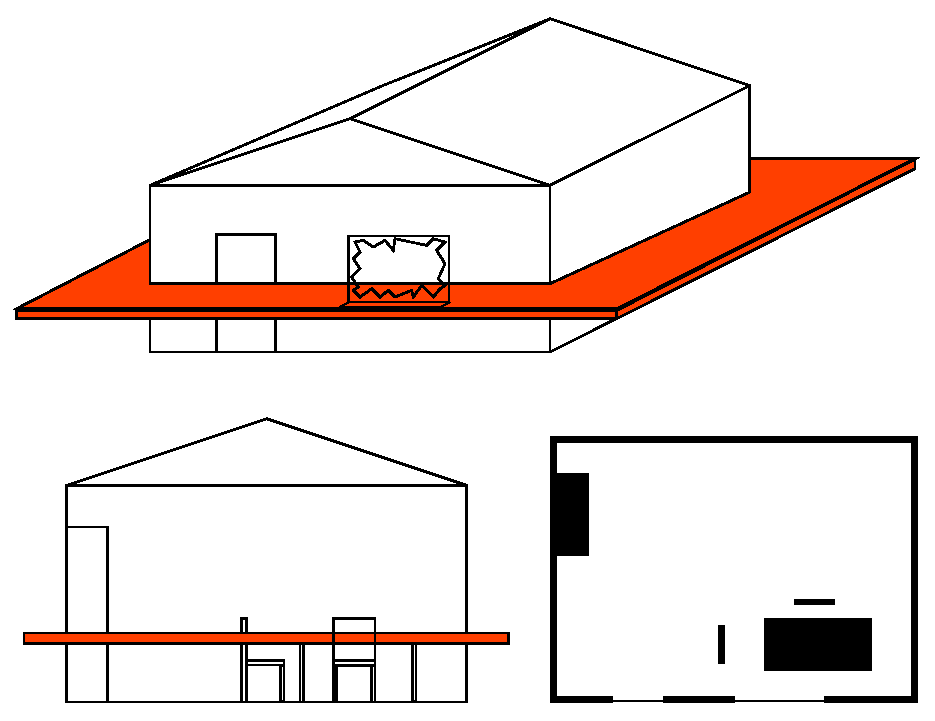
\includegraphics[clip=true,
    width=120mm]{FIGURES/evac_grid2}}
  \caption{A 2D evacuation mesh.}\label{Fig_EvacGrid} 
\end{figure}
%

\section{The \Timtt{MESH} Namelist Group}\label{Sec_EvacGrid}

\noindent The fire and evacuation meshes are separate ones.  One can do only a
fire calculation, only an evacuation calculation, or both at the same
time.  The calculation mode is chosen by activating the meshes or
deactivating them, \emph{i.e.}, commenting the corresponding \Timtt{\&MESH}
namelists out.

\begin{description}
%
\item[\Timtt{EVACUATION}] Should be \Timtt{.TRUE.} for all evacuation
  meshes.  Default is \Timtt{.FALSE.}
%
\item[\Timtt{EVAC\_HUMANS}] Should be \Timtt{.TRUE.} for all main
  evacuation meshes.  Default is \Timtt{.FALSE.}
%
\item[\Timtt{ID}] The specific ID string of this mesh.  An unique name
  should be given for each evacuation mesh.
%
\item[\Timts{EVAC\_Z\_OFFSET}] The distance from the mid height of the
  main evacuation mesh to the floor.  This parameter is used to show
  the bodies of the agents in Smokeview so that their feet are
  touching the floor (default is 1.0~m).  This needs to be given only
  for the main evacuation meshes.  This parameter also defines the
  reference floor level for the smoke and FED calculation, see the
  parameter \Timts{HUMAN\_SMOKE\_HEIGHT} on the \Timtt{PERS} namelist.
%
\end{description}

Evacuation mesh lines should have a keyword \Timtt{EVACUATION=.TRUE.}.
The default is \Timtt{.FALSE.}, \emph{i.e.}, the fire meshes do not
need the keyword \Timtt{EVACUATION}.  This is true also more
generally, \emph{i.e.}, one can always run a fire simulation even if
there exists evacuation input in the input file.  The FDS5 fire
calculation ignores all evacuation lines and keywords, if there is no
active evacuation meshes.

Main evacuation meshes should have also a keyword
\Timtt{EVAC\_HUMANS=.TRUE.} (default is \Timtt{.FALSE.}), which says
that this mesh will contain agents.  Usually, one main evacuation mesh
represents a 'floor'.  You need more main evacuation meshes on a floor
if there exists separate parts of the floor, where the agents are not
going to be using same exit routes.  If you have a main evacuation
mesh, where two or more parts are not directly connected by open
routes, then the flow field of that mesh is not nice.  Note also that
the evacuation calculation is faster if you define different meshes
for the parts, which do not interact with each other, because the
computational cost is additive between different meshes and inside one
mesh there are loops which scale as $N^2$, where $N $ is the number of
the agents.

All evacuation meshes should have a name, \emph{i.e.}, a keyword \Timtt{ID}
should be given on the \Timtt{\&MESH} line.  The name of the mesh
should not be too long, max 26 characters.  Of course, the names of
different meshes can not be the same.  The \Timtt{ID} is used later to
specify the mesh, where some additional evacuation objects are placed.

Evacuation meshes should have only one cell in the $z$ direction,
\emph{i.e.}, they are two dimensional horizontal meshes, see
Figure~\ref{Fig_EvacGrid}.  Choose \Timtt{IJK} and \Timtt{XB} so that
the $dx$ and $dy$ are nice round numbers that will fit nicely to your
geometry.  You should give the positions of all evacuation objects as
multiples of $dx$ and $dy$.  This is not obligatory but one makes less
mistakes this way.  The earlier FDS+Evac versions did not move the
evacuation objects to the closest mesh points, but the present version
(2.1.1) and onwards the namelists \Timtt{DOOR}, \Timtt{EXIT}, and
\Timtt{ENTR} are move to closest mesh points.

Evacuation meshes, which are only used to calculate the (additional)
evacuation movement flow fields towards different doors/exits should
have \Timtt{EVAC\_HUMANS=.FALSE.} or just no \Timtt{EVAC\_HUMANS}
keyword at all.  Note, that these meshes should have exactly the same
\Timtt{IJK} and \Timtt{XB} definitions as the corresponding main
evacuation meshes.  This is not (yet) checked by the program so the
user should do the check.
 

\section{The \Timtt{TIME} Namelist Group}

\begin{description}
%
\item[\Timts{EVAC\_DT\_FLOWFIELD}] is the time step of the calculation
  of the evacuation flow fields.  These fields are calculated before
  the fire and evacuation calculation, \emph{i.e.}, simulation time
  has negative values. (Default is 0.01~s.)
%
\item[\Timts{EVAC\_DT\_STEADY\_STATE}] is the maximum time step of the
  agent movement algorithm, this should not be too large, should not
  be larger than 0.1~s.  Note that the time step in the output files
  will not be shorter than this value.  This parameter defines the
  minimum coupling frequency of different main evacuation meshes.
  Coupling is faster if the time step of the fire calculation is
  shorter. (Default is 0.05~s.)
%
\end{description}



\section{The \Timtt{SURF} Namelist Group}

\noindent One should always define a new surface type for the evacuation
calculation, which is used to construct the flow fields that guide the
agents to the doors (or to other targets), see
Figure~\ref{Fig_EvacFlowField}.  The following line should be given on
the input file:
\begin{verbatim}
  &SURF ID = 'OUTFLOW', VEL = +0.000001, TAU_V=0.1 /  
\end{verbatim}
%
Note, that \Timtt{VEL} should be a really small number, otherwise one
might not get a nice 2D potential flow solution.




\section{The \Timtt{MISC} Namelist Group}

\begin{description}
%
\item[\Timts{EVACUATION\_MC\_MODE}] This parameter has only an effect
  when there are no fire meshes in the calculation.  If the EFF file
  is wanted to be read in then this keyword should be set to
  \Timtt{.TRUE.}.  The default is \Timtt{.FALSE.}, \emph{i.e.,} the
  evacuation flow fields are (re)calculated.
%
\item[\Timts{EVAC\_SURF\_DEFAULT}] is the surface default for the
  evacuation meshes.  The default is \Timtt{INERT}.  You could specify
  some other solid material for the default surface material, but
  FDS+Evac uses only the colour information.
%
\item[\Timts{EVAC\_PRESSURE\_ITERATIONS}] is the number of Poisson
  solver iterations at each evacuation flow field time step.  If you
  evacuation flow fields do not look nice, you might need to increase
  this.  A too large number makes the flow field calculation to take
  too much CPU time.  (Default is 50.)
%
\item[\Timts{EVAC\_TIME\_ITERATIONS}] is the number of evacuation flow
  field calculation time steps.  One should have a nice converged
  evacuation flow field, so some iterations are needed.  A too large
  number means too long CPU time.  (Default is 50.)
%
\end{description}

The flow fields, which are used to guide agents out of the building or
to some other targets, are calculated before the actual fire and
evacuation simulation, \emph{i.e.}, flow field calculation has $ t <
t_\textrm{start}$.  The product of the keywords $t_\mathrm{flow}=$
\Timts{EVAC\_TIME\_ITERATIONS} $\times$ \Timts{EVAC\_DT\_FLOWFIELD}
defines the duration of the evacuation flow field calculation.  The
fields should reach 'steady-state' during this time.  Note, that the
ramp up time of the boundary conditions \Timtt{TAU\_V=0.1} is given on
the \Timtt{\&SURF ID='OUTFLOW'} line and it should be well below the
duration of the flow field calculation $t_\mathrm{flow}$.  Default
$t_\mathrm{flow}$ is $50\times 0.01~\mathrm{s} = 0.5~\mathrm{s}$.




\section{The \Timtt{VENT} Namelist Group}


\begin{description}
%
\item[\Timtt{EVACUATION}] Should be \Timtt{.TRUE.} for all evacuation
  flow field vents used to generate the guiding flow field towards
  different exits and doors.  Default is \Timtt{.FALSE.}, \emph{i.e.},
  fire mesh vents are not noticed in the evacuation meshes.  There
  should be an evacuation \Timtt{VENT} defined at each exit/door on
  the main evacuation meshes, or otherwise the agents will not be able
  to use these doors.
%
\item[\Timtt{MESH\_ID}] This parameter is used to specify the
  evacuation mesh, where this \Timtt{VENT} is applied.
%
\end{description}

Because one needs to specify special \Timtt{VENT}s for the evacuation
calculation, the \Timtt{VENT} namelist group has an additional logical
item \Timtt{EVACUATION}.  If it is \Timtt{.TRUE.} then this
\Timtt{VENT} is omitted in the fire calculation.  The default value is
\Timtt{.FALSE.}, \emph{i.e.,} the fire calculation boundary conditions
are not used in the evacuation geometry.  The keyword \Timtt{MESH\_ID}
should also be given, if the \Timtt{VENT} is not needed in all
evacuation flow field calculations on this floor.  Note, that an
evacuation \Timtt{VENT} without \Timtt{MESH\_ID} is put on every
evacuation flow field on this floor.  This means that it is better
always to have the item \Timtt{MESH\_ID} specified, if
\Timtt{EVACUATION=.TRUE.} is given.  Note, that in FDS5 \Timtt{VENT}
must always be defined on a solid surface or on the outer boundary of
the computational domain.  Thus, the user may need to place additional
evacuation \Timtt{OBST}s behind the \Timtt{VENT}s used to generate the
evacuation flow fields.



\section{The \Timtt{OBST} Namelist Group}

\begin{description}
%
\item[\Timtt{EVACUATION}] Should be \Timtt{.TRUE.} for all evacuation
  mesh obstacles, which are not needed in the fire calculation.  If it
  is \Timtt{.FALSE.} then this \Timtt{OBST} is only applied in the
  fire calculation meshes.  Default is not defined, \emph{i.e.}, the
  \Timtt{OBST} is applied both to fire and evacuation meshes.
%
\item[\Timts{MESH\_ID}] This parameter is used to specify the
  evacuation mesh, where this \Timtt{OBST} is applied.
%
\end{description}

One may need to specify special \Timtt{OBST}s for the evacuation
calculation, which are not present in the fire calculation.  Thus, the
\Timtt{OBST} namelist group has an additional logical item
\Timtt{EVACUATION}.  If it is \Timtt{.TRUE.} then this \Timtt{OBST} is
omitted in the fire calculation.  If the evacuation flow fields need
different obstacles for different evacuation flow fields, then the
item \Timts{MESH\_ID} should be given for the evacuation obstacles.
Usually these additional evacuation obstacles are introduced at
places, where agents are not allowed to walk.



\section{The \Timtt{HOLE} Namelist Group}

\begin{description}
%
\item[\Timtt{EVACUATION}] Should be \Timtt{.TRUE.} for all evacuation
  mesh obstacles, which are not needed in the fire calculation.  If it
  is \Timtt{.FALSE.} then this \Timtt{HOLE} is only applied in the
  fire calculation meshes.  Default is not defined, \emph{i.e.}, the
  \Timtt{HOLE} is applied both to fire and evacuation meshes.
%
\item[\Timts{MESH\_ID}] This parameter is used to specify the
  evacuation mesh where this \Timtt{HOLE} is applied.
%
\end{description}

This is similar to the \Timtt{OBST} namelist group.  If the evacuation
flow fields need different holes for different fields, then the item
\Timtt{MESH\_ID} should be given for the evacuation calculation holes.



%
\begin{table}[!tp]
\begin{center}
\caption{Statistical distributions, which may be used to define the
  characteristics of the agents on the \Timtt{PERS} namelists.  The
  most used ones are: 0) no distribution, \Timtt{x\_MEAN} is used; 1)
  uniform distribution, \Timtt{x\_LOW} and \Timtt{x\_HIGH} are used;
  2) normal distribution, \Timtt{x\_MEAN} is the mean, \Timtt{x\_PARA}
  is the std.dev., \Timtt{x\_LOW} and \Timtt{x\_HIGH} are the cut
  offs, \emph{i.e.}, the values are within the interval
  (\Timtt{x\_LOW},\Timtt{x\_HIGH}).  If \Timtt{x\_LOW} is not given
  $\Rightarrow$ \Timtt{x\_LOW=0.0}.  If \Timtt{x\_HIGH} is not given,
  then \Timtt{x\_HIGH} is a 'very large' number.  Above, \Timtt{x}
  refers to one of the strings \Timts{DIA}, \Timts{VEL}, \Timts{TAU},
  \Timtt{DET}, or \Timtt{PRE}.  See
  Eqs.~\ref{Eq_GammaDist}--\ref{Eq_GumbelDist} for the definition for
  the distributions.}\label{Table_StatDists}
\vspace{12pt}
\begin{tabular}{l|c|c} \hline \hline
Distribution     & Index & Parameters \\ \hline 
No distribution  & 0 & \_MEAN ($x$) \\
Uniform          & 1 & \_LOW, \_HIGH ($x_\mathrm{min}$, $x_\mathrm{max}$) \\ 
Truncated normal & 2 & \_MEAN, \_PARA, \_LOW, \_HIGH ($\bar{x}$,
$\sigma$, $x_\mathrm{min}$, $x_\mathrm{max}$)  \\ 
Gamma            & 3 & \_PARA, \_PARA2 ($\alpha$, $\beta$) \\ 
Normal           & 4 & \_MEAN, \_PARA ($\bar{x}$, $\sigma$) \\ 
Log-normal       & 5 & \_MEAN, \_PARA, \_HIGH, \_PARA2, $\ln(x-x_0)$ normal distr. \\  
                 &   & ($\overline{\ln(x-x_0)}$,$\sigma_{\ln(x-x_0)}$,
                 $x_\mathrm{max}$, $x_0$) \\
Beta             & 6 & \_PARA, \_PARA2 ($\alpha$, $\beta$) \\ 
Triangular       & 7 & \_MEAN, \_LOW, \_HIGH ($x_\mathrm{peak}$,
$x_\mathrm{min}$, $x_\mathrm{max}$) \\  
Weibull          & 8 & \_PARA, \_PARA2 ($\alpha$, $\lambda$) \\ 
Exponential      & 8 & \_PARA=1, \_PARA2 ($\alpha$=1, $\lambda$) \\ 
Gumbel           & 9 & \_PARA ($\alpha$) \\ \hline \hline
\end{tabular}
\end{center}
\end{table}
%


\section{The \Timtt{PERS} Namelist Group}

\noindent This namelist group is used to define agent types.  Properties like
body diameters, walking speeds, pre-evacuation times, and force
constants of the agents are given here.  Some of the values might be
given as distributions.  There are five default agent types defined
and they are 'Adult', 'Male', 'Female', 'Child', and 'Elderly', see
Table~\ref{Table_DefaultHumans} for their body sizes and walking
speeds.  Note, that the body sizes and walking speeds are generated
from uniform distributions, whose ranges are also given in the table.
The default values of the other agent related parameters are listed at
the end of Ch.~\ref{Sec_MoveModel}.  The user should not usually
change any of the optional parameters.  It is enough to give some
predefined agent type and set the detection and reaction time
distributions.  Sometimes also the parameter \Timts{L\_NON\_SP} could
be set to a value of 0.3, see Chapters~\ref{Sec_ModelSensi} and
\ref{Sec_ModelValid}.  

This namelist is also used to set some miscellaneous (global)
parameters for evacuation calculation, which need to be given only on
some \Timtt{PERS} namelist group.

\begin{description}
%
\item[\Timtt{DEFAULT\_PROPERTIES}] 'Adult', 'Male', 'Female', 'Child',
  or 'Elderly'.  If not given, default values are used, see the end of
  Sec.~\ref{Sec_MoveModel}.  Note, that the default values of these
  agent types may be overridden if the various values are explicitly
  given in the \Timtt{PERS} namelists.
%
\item[\Timtt{DET\_EVAC\_DIST}] The type index of the detection time
  distribution, see Table~\ref{Table_StatDists} and
  Section~\ref{Sec_TdetTpre}.
%
\item[\Timtt{DET\_MEAN,DET\_PARA,DET\_PARA2,DET\_LOW,DET\_HIGH}] The
  parameters of the detection time distribution, see
  Table~\ref{Table_StatDists}.
%
\item[\Timtt{PRE\_EVAC\_DIST}] The type index of the reaction time
  distribution, see Table~\ref{Table_StatDists} and
  Section~\ref{Sec_TdetTpre}.
%
\item[\Timtt{PRE\_MEAN,PRE\_PARA,PRE\_PARA2,PRE\_LOW,PRE\_HIGH}] The
  parameters of the reaction time distribution, see
  Table~\ref{Table_StatDists}.
%
\item[\Timts{DIAMETER\_DIST}] The type index of the body size
  distribution, see Table~\ref{Table_StatDists}.  Note, that the
  distribution is given for the diameter of the large body circle,
  which encircles the whole body ellipse, see
  Figure~\ref{Fig_HumanBody}.
%
\item[\Timts{DIA\_MEAN,DIA\_PARA,DIA\_PARA2,DIA\_LOW,DIA\_HIGH}] The
  parameters of the distribution used for the diameter of the agent
  circle ($2R_d$), see Figure~\ref{Fig_HumanBody} and
  Tables~\ref{Table_DefaultHumans} and \ref{Table_StatDists}.
%
\item[\Timts{VELOCITY\_DIST}] The type index of the unimpeded walking
  speed distribution, see Table~\ref{Table_StatDists}.
%
\item[\Timts{VEL\_MEAN,VEL\_PARA,VEL\_PARA2,VEL\_LOW,VEL\_HIGH}] The
  parameters of the target walking speed, $v_i^0$, distribution, see
  Eq.~\ref{Eq_force} and Tables~\ref{Table_DefaultHumans} and
  \ref{Table_StatDists}.
%
\item[\Timts{TAU\_EVAC\_DIST}] The type index of the relaxation time
  parameter distribution, see Table~\ref{Table_StatDists}.
%
\item[\Timts{TAU\_MEAN,TAU\_PARA,TAU\_PARA2,TAU\_LOW,TAU\_HIGH}] The
  parameters of the relaxation time, $\tau_i$, distribution, see
  Eq.~\ref{Eq_force} and Table~\ref{Table_StatDists}.
%
\item[\Timts{FCONST\_A,FCONST\_B,L\_NON\_SP}] Social force parameters
  $A_i$, $B_i$, $\lambda_i$, see Eq.~\ref{Eq_socialforce}.
%
\item[\Timts{C\_YOUNG,KAPPA}] Contact force parameters $k_i$ and
  $\kappa_i$, see Eq.~\ref{Eq_contactforce}.
%
\item[\Timts{D\_TORSO\_MEAN,D\_SHOULDER\_MEAN}] The mean diameters of
  the torso and shoulder circles, see Table~\ref{Table_DefaultHumans}
  and Figure~\ref{Fig_HumanBody}.  The variations of these diameters are
  determined by the diameter distribution of the agent circle
  ($2R_d$).
%
\item[\Timts{TAU\_ROT}] The relaxation time, $\tau_i^z$, for the
  rotational equation of motion, see Eq.~\ref{Eq_motive_torque}.
%
\item[\Timts{M\_INERTIA}] The moment of inertia, $I_i^z$, for the rotational
  equation of motion, see Eq.~\ref{Eq_rotmotion}.
%
\end{description}
%
% Below are just given on one PERS-line (values last )
%
NOTE: For the keywords listed below, only the last values read from
\Timtt{PERS} namelists are used.  So, it is nice practice to give
these keywords just on one \Timtt{PERS} namelist group or have exactly
same values on every \Timtt{PERS} namelist group.  Some of these
keywords set some global model parameters for all agents and some are
used to specify the outputs and the mode of operation of the
programme.
%
\begin{description}
%
\item[\Timts{FAC\_A\_WALL}] Social force constant $A_w$ for
  wall--agent interaction is \Timtt{FAC\_A\_WALL}$\times A_i$.
%
\item[\Timts{FAC\_B\_WALL}] Social force constant $B_w$ for
  wall--agent interaction is \Timtt{FAC\_B\_WALL}$\times B_i$.
%
\item[\Timts{LAMBDA\_WALL}] Social force constant $\lambda_w$ for
  wall--agent interaction.
%
\item[\Timts{FC\_DAMPING}] Damping coefficient $c_d$ of the radial
  contact force, see Eq.~\ref{Eq_contactforce}.
%
\item[\Timts{V\_ANGULAR}] Maximum target angular speed of the agents,
  $\omega^0$, see Eq.~\ref{Eq_motive_torque}.
%
\item[\Timts{NOISEME,NOISETH,NOISECM}] Gaussian noise, see
  Eqs.~\ref{Eq_motion} and \ref{Eq_rotmotion}.  These parameters
  determine both the noise in the translational equation,
  ${\boldsymbol \xi}_i$ in Eq.~\ref{Eq_motion}, and the noise in the
  rotational equation, ${\eta}^z_{i}$ in Eq.~\ref{Eq_rotmotion}.
%
%\item[\Timts{I\_FRIC\_SW}] Friction force switch:\\
%  1: $\kappa (d_{ij} - r_{ij}) \Delta v_{ij}^{t} \mathbf{t}_{ij}$~~
%  Default value, \\ 
%  0: $\gamma \Delta v_{ij}^{t} \mathbf{t}_{ij}$
%
\item[\Timts{HUMAN\_SMOKE\_HEIGHT}] Specifies the level above the
  floor, where the smoke and FED information is taken.  Note, that the
  parameter \Timts{EVAC\_Z\_OFFSET} and the coordinates \Timtt{XB} on
  the evacuation mesh namelists define the floor levels.  (Default is
  1.6~m.)
%
\item[\Timts{TDET\_SMOKE\_DENS}] If > 0.0 then an agent detects the
  fire when the smoke density ($\mathrm{mg/m^3}$) is larger than the
  given value at the position of the agent if the agent has not yet
  detected the fire due to the detection time distribution.  Default
  is no detection by smoke.
%
\item[\Timts{FED\_DOOR\_CRIT}] This sets the amount of ``smoke'' which
  is used to decide if some door is considered to be ``smoke free'' in
  the door selection algorithm of FDS+Evac.  If > 0.0 then a door is
  considered to be smoke free, if the estimated FED value for this
  agent is less than the given value.  If < 0.0 then the absolute
  value is the visibility distance (m) which is used by the door
  selection algorithm to rank a door as smoke free (visibility $S =
  3/K$). See Sec.~\ref{Sec_FireHumanInt}.  Default is 0.000001.
%
\item[\Timts{SMOKE\_MIN\_SPEED}] This sets the minimum speed of the
  agents when they are moving in smoke, $v^0_{i,\mathrm{min}} =
  \Timts{SMOKE\_MIN\_SPEED} \times v^0_i$ in Eq.~\ref{Eq_SpeedSmoke}.
  Default is 0.1.
%
\item[\Timts{DENS\_INIT}] If > 2.0, then agents are tried to put on
  the initial positions so that they can be touching.  The default is
  to leave some space between agents and very large agent densities
  are not possible.  Note that FDS+Evac puts agents randomly in their
  initial positions and, thus, the initial density of agents can not
  be much larger than four agents per square meter.  Default is 0.0.
%
\item[\Timts{EVAC\_DT\_MAX}] The maximum time step for the agent
  movement algorithm, default 0.01~s.
%
\item[\Timts{EVAC\_DT\_MIN}] The minimum time step for the agent
  movement algorithm, default 0.001~s.
%
\item[\Timts{NOT\_RANDOM}] If \Timtt{.TRUE.} do not use random seed
  when generating the initial positions and characteristics of agents.
  Default is \Timtt{.FALSE.}
%
\item[\Timts{COLOR\_METHOD}] How agents are shown in Smokeview. -1:
  use standard colors in Smokeview, 0: use avatar colors given on the
  \Timtt{EVAC} lines, 3: use avatar colors given on the \Timtt{PERS}
  lines, 4: color the agents according the target door/exit colors, 5:
  color the agents according the exit selection algorithm, see
  Table~\ref{Table_pref_order}.  The default is -1.
%
\item[\Timts{AVATAR\_COLOR}] Color of the agents seen in Smokeview if
  \Timts{COLOR\_METHOD=3}.  See the FDS User's Guide and FDS web page
  for the list of available color names.
%
\item[\Timts{AVATAR\_RGB}] Three integers (0--255) specifying a color
  of the agents seen in Smokeview if \Timts{COLOR\_METHOD=3}.  Note,
  that \Timts{AVATAR\_COLOR} overrides this option.
%
\item[\Timts{DEAD\_COLOR}] Color of the dead agents seen in Smokeview.
  See the FDS User's Guide and FDS web page for the list of available
  color names.  Default color for dead agents is cyan.
%
\item[\Timts{DEAD\_RGB}] Three integers (0--255) specifying a color of
  the dead agents seen in Smokeview.  Note, that \Timts{DEAD\_COLOR}
  overrides this option.  Default color for dead agents is cyan.
%
\item[\Timts{OUTPUT\_SPEED}] If \Timtt{.TRUE.} then the movement
  speeds of the agents are saved in the ouput file to be shown in
  Smokeview as a color bar.
%
\item[\Timts{OUTPUT\_FED}] If \Timtt{.TRUE.} then the FED doses of the
  agents are saved in the ouput file to be shown in Smokeview as a
  color bar.
%
\item[\Timts{OUTPUT\_CONTACT\_FORCE}] If \Timtt{.TRUE.} then the
  contact forces acting on the circumferences (N/m) of the agents are
  saved in the ouput file to be shown in Smokeview as a color bar.
%
\item[\Timts{OUTPUT\_TOTAL\_FORCE}] If \Timtt{.TRUE.} then the total
  forces (contact + social) acting on the circumferences (N/m) of the
  agents are saved in the ouput file to be shown in Smokeview as a
  color bar.
%
\end{description}

Below the probability density functions are listed for those
distributions in Table~\ref{Table_StatDists}, where the naming of the
parameters is not trivial.

The definition of the probability density function of the Gamma
distribution is:
%
\begin{equation}\label{Eq_GammaDist}
 f(x) =  \frac{1}{\Gamma(\alpha)\beta^\alpha} ~ x^{\alpha-1}
 e^{-x/\beta} ~,~ x > 0 ,~ \alpha,\beta > 0
\end{equation}
%
The definition of the probability density function of the Normal
distribution is:
%
\begin{equation}\label{Eq_NormalDist}
 f(x) = \frac{1}{ \sigma \sqrt{2\pi}} ~ \exp \left\{ -
 \frac{(x-\bar{x})^2}{2 \sigma^2} \right\}   ~,~ \sigma > 0
\end{equation}
%
The definition of the probability density function of the Log-Normal
distribution is:
%
\begin{equation}\label{Eq_LogNormalDist}
 f(x) = \frac{\mathrm{const}}{(x-x_0) \sigma \sqrt{2\pi}} ~ \exp \left\{ -
 \frac{(\ln(x-x_0)-\mu)^2}{2\sigma}  \right\}   ~,~ \sigma > 0,~ x < x_\mathrm{max}
\end{equation}
where $\mu$ and $\sigma$ are the mean and the standard deviation of
$\ln(x-x_0)$, respectively. 
%
%Log-normal 
%%
%\begin{equation}
% \ln(x) \textrm{has normal distribution}~ N(\bar{\ln(x)},\sigma_{\ln(x)})
%\end{equation}
%
The definition of the probability density function of the Beta
distribution is:
%
\begin{equation}\label{Eq_BetaDist}
 f(x) = \mathrm{const} \cdot x^{\alpha-1} (1-x)^{\beta-1}  ~,~  x \in
 [0;1] ,~ \alpha,\beta > 0 
\end{equation}
%
The definition of the probability density function of the Weibull 
distribution is:
%
\begin{equation}\label{Eq_WeibullDist}
 f(x) = \alpha\lambda(\lambda x)^{\alpha-1} \exp(-(\lambda x)^\alpha) ~,~ x
 \geq 0 ,~ \alpha,\lambda > 0
\end{equation}
% Weibull: nolla, jos x<0
%
The definition of the probability density function of the Exponential
distribution is:
%
\begin{equation}\label{Eq_ExpDist}
 f(x) =  \lambda e^{-\lambda x} ~,~ x\geq 0 ,~ \lambda > 0
\end{equation}
%
The definition of the probability density function of the Gumbel
distribution is:
%
\begin{equation}\label{Eq_GumbelDist}
 f(x) =  \alpha e^{-\alpha x} \exp( -e^{-\alpha x} ) ~,~ \alpha > 0
\end{equation}
%

\noindent WARNING: Change only the reaction and detection time
parameters, other parameters should have the default values and use
the predefined person types, unless you know what you are doing.  The
parameter \Timts{L\_NON\_SP} may be changed from its default value 0.5
to a value 0.3, if a more relaxed egress is wanted, see
Chapters~\ref{Sec_ModelSensi} and \ref{Sec_ModelValid}.

 
\section{The \Timtt{EVAC} Namelist Group}

\noindent Places agents in the evacuation meshes, \emph{i.e.}, this
namelist group is used to define the initial positions of the agents.
%
\begin{description}
%
\item[\Timtt{ID}] ID string of the group of agents.
%
\item[\Timtt{XB}] Defines the rectangle, where the agents are put, $z$
  should belong to the correct main evacuation mesh.  If the
  coordinates \Timtt{XB} intersects many evacuation meshes then the
  keyword \Timts{MESH\_ID} should be given.
%
\item[\Timts{MESH\_ID}] If there are overlapping main evacuation
  meshes then this parameter could be used to specify the mesh, where
  this \Timtt{EVAC} namelist is applied.
%
\item[\Timtt{NUMBER\_INITIAL\_PERSONS}] How many persons are put in
  the rectangle \Timtt{XB}.
%
\item[\Timtt{PERS\_ID}] The \Timtt{ID} string of the \Timtt{PERS}
  namelist, which is used to define the characteristics of the
  (randomly) generated agents.
%
\item[\Timts{ANGLE}] By default the orientation of agents is random,
  but by giving an angle (0--360) the orientation of the agents can be
  specified.  Angle 0 means that the agents are facing towards +$x$
  and the positive direction of the angle is anti-clockwise.
%
%\item[\Timts{QUANTITY}] Colour of the torso of the agents in Smokeview.
%  The colours which can be used are: black, yellow, blue, red, green,
%  magenta, and cyan.  Note, that if a person is dead, it is coloured as
%  \Timtt{CYAN}.  Default is \Timtt{BLACK}.
%
\item[\Timts{AVATAR\_COLOR}] Colour of the agents seen in Smokeview if
  \Timts{COLOR\_METHOD=0}.  See the FDS User's Guide and FDS web page
  for the list of available colour names.
%
\item[\Timts{AVATAR\_RGB}] Three integers (0--255) specifying a colour
  of the agents seen in Smokeview if \Timts{COLOR\_METHOD=0}.  Note,
  that \Timts{AVATAR\_COLOR} overrides this option.
%
%\item[\Timts{FLOW\_FIELD\_ID}] Specifies which evacuation flow field
%  the agents are following if there are no known nor visible doors
%  available at the main evacuation mesh, where the agents are placed.
\item[\Timts{FLOW\_FIELD\_ID}] The ID of a MESH namelist that defines
  the evacuation flow field the agents are following if there are no
  known nor visible doors available at the main evacuation mesh, where
  the agents are placed.  By default it is the ID of the main
  evacuation mesh, \emph{i.e.} the agents are ``flowing'' towards all the
  exits.
%
\item[\Timts{KNOWN\_DOOR\_NAMES}] The \Timtt{ID} strings of the known
  doors and exits for the agents.
%
\item[\Timts{KNOWN\_DOOR\_PROBS}] The probabilities that the exit
  doors are known.  At the initialisation phase the known doors for
  agents are drawn using these probabilities.  Default values are
  equal to ones, \emph{i.e.}, the listed known doors will be known to
  all agents generated by this \Timtt{EVAC} namelist.
%
\end{description}

\noindent NOTE: If no \Timtt{PERS\_ID} is given on \Timtt{EVAC} lines,
then the default values are used for the properties of persons.  These
default values are given inside the programme source code, and they
might be changing during the development of the programme.  So, one
should not use the default values.


\section{The \Timtt{EVHO} Namelist Group}

\noindent Specifies a place where no agents are generated by the \Timtt{EVAC}
namelists.
%
\begin{description}
%
\item[\Timtt{ID}] ID string of the hole.  One can refer to this hole
  by its name.
%
\item[\Timtt{XB}] Defines the rectangle, where the agents are not put,
  $z$ should belong to a main evacuation mesh.  If \Timtt{XB}
  intersects many evacuation meshes then the keyword \Timts{MESH\_ID}
  should be given.
%
\item[\Timts{MESH\_ID}] If there are overlapping main evacuation
  meshes then this parameter could be used to specify the mesh, where
  this \Timtt{EVHO} namelist is applied.
%
\item[\Timts{PERS\_ID}] This hole applies just for this person type,
  \emph{i.e.}, it has effect only on those \Timtt{EVAC} namelists,
  where \Timts{PERS\_ID} matches.
%
\item[\Timts{EVAC\_ID}] This hole applies just for the given \Timtt{EVAC}
  namelist.  If both \Timts{PERS\_ID} and \Timts{EVAC\_ID} are given, they
  are treated using the logical operator OR.
%
\end{description}



\section{The \Timtt{EXIT} Namelist Group}

\noindent Defines an exit, which removes agents from the calculation
for good.  Note, that an 'outflow' vent is not automatically created,
so the user should give a separate \Timtt{VENT} namelist for each
exit.  Exits might be used just to count agents, then the keyword
\Timts{COUNT\_ONLY=.TRUE.}  is used and, thus, these can be placed
anywhere inside the building.  Agents, which move through an exit
(\Timts{COUNT\_ONLY=.FALSE.}), are removed from the calculation,
\emph{i.e.}, they are supposed to be gone outside of the building and
be safe.

\begin{description}
%
\item[\Timtt{ID}] ID string of the exit.  One can refer to this exit by
  its name.
%
\item[\Timtt{XB}] Defines the position of the exit, should be a line
  in the $(x,y)$ plane, the $z$ should belong to a main evacuation
  mesh.  If \Timtt{XB} intersects many evacuation meshes then the
  keyword \Timts{MESH\_ID} should be given.  Note, that the FDS+Evac
  versions 2.1.1. and later are moving the corners of the rectangle
  defined by \Timtt{XB} to the closest grid cell corners.
%
\item[\Timts{MESH\_ID}] If there are overlapping main evacuation
  meshes then this parameter could be used to specify the mesh where
  this exit is applied.
%
\item[\Timts{XYZ}] Coordinates, which are used in the exit door
  selection algorithm to decide if the exit is visible or not.
  Default is the mid-point of \Timtt{XB}.
%
\item[\Timtt{IOR}] Direction of the door, \emph{e.g.}, +1 agents are
  going $+x$ direction, -2 agents are going $-y$ direction (direction
  means: room $\Rightarrow$ exit $\Rightarrow$ outside of the
  building)
%
\item[\Timts{COUNT\_ONLY}] If \Timtt{.TRUE.}, agents are not removed,
  they are just counted (default is \Timtt{.FALSE.}).  The
  \Timtt{CHID\_evac.csv} file has a column for each \Timtt{EXIT}
  regardless if \Timts{COUNT\_ONLY} is true or false.
%
\item[\Timts{VENT\_FFIELD}] The \Timtt{ID} string of the evacuation
  flow field mesh behind this exit door.  The agents are guided to
  this exit door by the specified flow field.  If none is given then
  the agents, whose target this exit is, are following the flow field
  of the current main evacuation mesh, \emph{i.e.,} they are just
  going where the flow goes and not towards this exit.  This parameter
  should be given if the exit selection algorithm of FDS+Evac is being
  used.
%
\item[\Timts{FLOW\_FIELD\_ID}] Used, if this exit is a target for some
  other evacuation element and there are no known doors nor visible
  ones available.  If \Timts{FLOW\_FIELD\_ID} is not given, then the
  main evacuation mesh flow field is used.  WARNING: It is better to
  use a door or an entry instead of an exit if it is a target of some
  other evacuation element.
%
\item[\Timts{COLOR}] Colour of the agents seen in Smokeview if
  \Timts{COLOR\_METHOD=4}.  See the FDS User's Guide and FDS web page
  for the list of available colour names.
%
\item[\Timts{RGB}] Three integers (0--255) specifying a colour of the
  agents seen in Smokeview if the \Timts{COLOR\_METHOD=4} is specified
  on (some) \Timtt{PERS} namelist.  Note, that the \Timts{COLOR}
  keyword overrides this option.
%
%\item[\Timts{COLOR\_INDEX}] Colour index of the torso of the agent in
%  Smokeview if the \Timtt{COLOR\_METHOD}=4 on \Timtt{PERS} namelist.
%  The colours which can be used are: black (0), yellow(1), blue(2),
%  red(3), green(4), magenta(5), and cyan(6).  Default is 0.
%
\item[\Timts{TIME\_OPEN}] The time (s) when this exit becomes usable.
  The default is that the exit is always usable.
%
\item[\Timts{TIME\_CLOSE}] The time (s) when this exit becomes
  unusable.  The default is that the exit is always usable.
%
\end{description}


\section{The \Timtt{ENTR} Namelist Group}

\noindent Defines an entry.  An entry can enter agents to the calculation at a
constant frequency.  An entry with frequency zero can just be used as
an end point of a corridor or stairs.  An entry corresponds to a one
way door, \emph{i.e.}, agents can only come out from this 'door'.

\begin{description}
%
\item[\Timtt{ID}] ID string of the entry.  One can refer to this entry
  by its name.
%
\item[\Timtt{XB}] Defines the position of the entry, should be a line
  in the $(x,y)$ plane, the $z$ should belong to a main evacuation
  mesh.  If \Timtt{XB} intersects many evacuation meshes then the
  keyword \Timts{MESH\_ID} should be given.  Note, that the FDS+Evac
  versions 2.1.1. and later are moving the corners of the rectangle
  defined by \Timtt{XB} to the closest grid cell corners.
%
\item[\Timts{MESH\_ID}] If there are overlapping main evacuation
  meshes then this parameter could be used to specify the mesh where
  this \Timtt{ENTR} line is applied.
%
\item[\Timtt{IOR}] The direction of the entry, \emph{e.g}., +1 agents
  are entering towards $+x$ direction -2 agents are entering towards
  $-y$ direction (direction means: somewhere $\Rightarrow$ entry
  $\Rightarrow$ room).  Note that the namelist \Timtt{EXIT} has just
  the opposite rule for the sign of \Timtt{IOR}.
%
\item[\Timts{MAX\_FLOW}] How many agents per second are introduced in
  the calculation. The actual flow may be smaller, if the area in
  front of the entry is crowded.  The default is zero.
%
\item[\Timtt{MAX\_HUMANS}] The maximum number of agents to be
  introduced in the calculation by this entry, the default is a very
  large integer.
%
\item[\Timts{TIME\_START}] The time (s) when this entry starts adding
  agents to the calculation.  The default is the starting time of the
  simulation, the \Timts{T\_BEGIN} keyword given on the  \Timtt{TIME}
  namelist group.
%
\item[\Timts{TIME\_STOP}] The time (s) when this entry stops adding
  agents to the calculation.  The default is that an entry never stops
  introducing new agents to the calculation.
%
\item[\Timtt{PERS\_ID}] The properties of agents are generated using
  these parameters, if they are not coming to this entry form some
  other node, \emph{i.e.}, they are 'new' agents.  If not given, the
  default values are used.
%
\item[\Timts{FLOW\_FIELD\_ID}] Flow field in the 'room/floor', which
  the agents are following after their entry, \emph{i.e.}, specifies
  to which door the agents try to go if no known nor visible doors are
  available.  If not given, the flow field of the main evacuation mesh
  is used.
%
\item[\Timts{KNOWN\_DOOR\_NAMES}] The ID strings of the known exit
  doors.  This only apply to agents that are generated at this entry
  by the \Timtt{MAX\_FLOW}, \emph{i.e.}, it does not apply to those
  agents who are transfered to this entry from somewhere else.
%
\item[\Timts{KNOWN\_DOOR\_PROBS}] The probabilities that the exit
  doors are known.  Only values equal to one or zero can be used for
  entries.  Default values are equal to ones.
%
\item[\Timts{AVATAR\_COLOR}] Colour of the agents seen in Smokeview if
  \Timts{COLOR\_METHOD=0}.  See the FDS User's Guide and FDS web page
  for the list of available colour names.
%
\item[\Timts{AVATAR\_RGB}] Three integers (0--255) specifying a colour
  of the agents seen in Smokeview if \Timts{COLOR\_METHOD=0}.  Note,
  that the \Timts{AVATAR\_COLOR} keyword overrides this option.
%
\end{description}



\section{The \Timtt{DOOR} Namelist Group}

\noindent Defines a door.  Similar to \Timtt{EXIT}, but the agents are not
removed from the calculation.  The agents are put to some other part
of the calculation, \emph{e.g.}, to stairs or to a different 'room'.

\begin{description}
%
\item[\Timtt{ID}] ID string of the door. One can refer to this door by
  its name.
%
\item[\Timtt{XB}] Defines the position of the door, should be a line in
  the $(x,y)$ plane, the $z$ should belong to a main evacuation mesh.
  If \Timtt{XB} intersects many evacuation meshes then the keyword
  \Timts{MESH\_ID} should be given.  Note, that the FDS+Evac versions
  2.1.1. and later are moving the corners of the rectangle defined by
  \Timtt{XB} to the closest grid cell corners.
%
\item[\Timts{XYZ}] Coordinates, which are used in the exit door
  selection algorithm to decide if the door is visible or not.
  Default is the mid-point of \Timtt{XB}.
%
\item[\Timts{MESH\_ID}] If there are overlapping main evacuation
  meshes then this parameter could be used to specify the mesh where
  this door is applied.
%
\item[\Timtt{IOR}] Direction of the door, \emph{e.g.}, +1 agents are
  going $+x$ direction, -2 agents are going $-y$ direction (direction
  means: room $\Rightarrow$ door $\Rightarrow$ some other place).
  Note that the namelist \Timtt{EXIT} has the same rule for the sign
  of \Timtt{IOR}.
%
\item[\Timtt{TO\_NODE}] Where agents are going, when going inside this
  door.  \Timtt{TO\_NODE} can be \Timtt{DOOR, EXIT, CORR,} or
  \Timtt{ENTR} namelist \Timtt{ID}.
%
\item[\Timts{EXIT\_SIGN}] If \Timtt{.TRUE.} then this door is
  considered as an ``exit door'' in the door selection algorithm.
  Agents can use this door even if it is not described as ``known
  door'', \emph{i.e.}, it can be classified as a ``visible, unknown
  door'' in the door selection algorithm. (Default is \Timtt{.FALSE.})
%
\item[\Timts{KEEP\_XY}] saves the information on the position of the
  agent relative to the width of the door, \emph{i.e.}, if the target
  of this door is a \Timtt{DOOR} or an \Timtt{ENTR} then the agent is
  placed according to this information.  If this is not set true, then
  the algorithm seeks randomly empty space in front of the target
  node.  One should set this true, if one is modelling stairs or
  spectator stands using \Timtt{EVSS}.  Default is \Timtt{.FALSE.}
%
\item[\Timts{VENT\_FFIELD}] The \Timtt{ID} string of the evacuation
  flow field mesh behind this door.  The agents are guided to this
  door by the specified flow field.  If none is given then the agents,
  whose target this door is, are following the flow field of the
  current main evacuation mesh, \emph{i.e.,} they are just going where
  the flow goes and not towards this door.  This parameter should be
  given if the exit selection algorithm of FDS+Evac is being used.
%
\item[\Timts{FLOW\_FIELD\_ID}] Used, if this door is a target for some
  other evacuation element and there are no known doors nor visible
  ones available.  If no \Timtt{FLOW\_FIELD\_ID} is given, then the
  main evacuation mesh flow field of this floor is used.
%
\item[\Timts{COLOR}] Colour of the agents seen in Smokeview if
  \Timts{COLOR\_METHOD=4}.  See the FDS User's Guide and FDS web page
  for the list of available colour names.
%
\item[\Timts{RGB}] Three integers (0--255) specifying a colour of the
  agents seen in Smokeview if the \Timts{COLOR\_METHOD=4} is specified
  on (some) \Timtt{PERS} namelist.  Note, that the \Timts{COLOR}
  keyword overrides this option.
%
\item[\Timts{TIME\_OPEN}] The time (s) when this door becomes usable.
  The default is that the door is always usable.
%
\item[\Timts{TIME\_CLOSE}] The time (s) when this door becomes
  unusable.  The default is that the door is always usable.
%
\end{description}



\section{The \Timtt{CORR} Namelist Group}

\noindent Defines stairs (or a horizontal corridor).  Namelists
\Timtt{CORR} are used to move agents from one floor to the next one,
\emph{i.e.}, from one main evacuation mesh to some other one.  The
corridor (actually stairs) model is a really simple one.  One gives
the length of the stairs and reduces the movement speed of the agents.
One also gives the maximum number of persons inside the corridor.  For
now there is no relation between the density and the movement speed
(nor specific flow) inside the stairs.

\begin{description}
%
\item[\Timtt{ID}] ID string of the corridor. One can refer to this
  \Timtt{CORR} by its name.
%
\item[\Timtt{MAX\_HUMANS\_INSIDE}] how many agents fit inside the
  corridor.  A rule of thumb: two persons per square metre.
%
\item[\Timtt{TO\_NODE}] Where agents are going, when leaving this
  corridor. \Timtt{TO\_NODE} can be \Timtt{DOOR}, \Timtt{ EXIT},
  \Timtt{CORR}, or \Timtt{ENTR} namelist \Timtt{ID}.
%
\item[\Timtt{XB}, \Timtt{XB1}, \Timtt{XB2}] Used to specify the
  points, where FED data is taken for this corridor/stairs.  If only
  one value is used for the corridor/stairs, give \Timtt{XB}.  If the
  values at the beginning and at the end of the corridor/stair is
  used, give both \Timtt{XB1} and \Timtt{XB2}, respectively, and the
  FED data values are linearly interpolated between the start and the
  end of the corridor/stairs.
%
\item[\Timts{FAC\_SPEED}] How much slower agents move in the
  corridor/stairs compared to the walking speed $v_i^0$ in horizontal
  floors.  (Default is 1.0)
%
\item[\Timtt{EFF\_LENGTH}] The effective length of the
  corridor/stairs.  The movement time of the agents inside the stairs
  is calculated as \Timtt{EFF\_LENGTH}/(\Timts{FAC\_SPEED}$\times
  v_i^0$).
%
\end{description}
%
Note, that \Timtt{CORR} is usually used to define stairs between two
floors: $\mathrm{Door_{2^{nd} ~floor}} ~ \rightarrow$ $\mathrm{Corr} ~
\rightarrow$ $\mathrm{Door_{1^{st} ~floor}}$.  Stairs could also be
constructed using the \Timtt{EVSS} namelists, but this is not as
straight forward as to use \Timtt{CORR} constructions.  See the
example input files on the FDS+Evac web pages.  If you have merging
flows in stairs, then you should model the landings explicitly and
you can use \Timtt{CORR} to move the agents from one landing to the
next one.



\section{The \Timtt{EVSS} Namelist Group}

\noindent Defines an incline, \emph{e.g.}, stairs, a spectator stand, or an
escalator.  The defined ``incline'' could also be horizontal.  Then it
specifies a piece of the current floor at different vertical position
than given on the \Timtt{MESH} line of the evacuation floor.  This way
intermediate landings in stairs could be modelled, see the ``stairs''
example case on the FDS+Evac web pages.  The \Timtt{EVSS} namelists
just change the $z$ coordinates of the agents, when these are saved
on the hard disk to be plotted by Smokeview.  Thus, the internal agent
movement algorithm of FDS+Evac does not use the $z$ coordinates.  All
agents on a given main evacuation mesh are always projected to the
same horizontal plane.  \Timtt{EVSS} can also be used just to change
the movements speeds of the agents at some parts of the floor.

\begin{description}
%
%
\item[\Timtt{ID}] ID string of the incline.
%
\item[\Timtt{XB}] Defines the position of this ``incline'', should
  define a rectangle in the $(x,y)$ plane, the $z$ should belong to a
  main evacuation mesh.  If \Timtt{XB} intersects many main evacuation
  meshes then the keyword \Timts{MESH\_ID} should be given.
%
\item[\Timtt{IOR}] Direction of the incline, \emph{e.g.}, +1 means
  that the +$x$ edge of the EVSS plane is a horizontal line at a
  height \Timts{HEIGHT0} above (or below if < 0~m) the main evacuation
  plane defined by the $z$ of \Timtt{XB} and the -$x$ edge is a
  horizontal line a height \Timts{HEIGHT} above (or below if < 0~m)
  the main evacuation plane.
%
\item[\Timts{MESH\_ID}] If there are overlapping main evacuation
  meshes then this parameter could be used to specify the mesh where
  this \Timtt{EVSS} line is applied.
%
\item[\Timts{HEIGHT}] The height of the ``\Timtt{-IOR}'' edge of the
  incline measured from the level of the main evacuation plane defined
  by the $z$ of \Timtt{XB}.  This edge has $z = z_{\scriptscriptstyle
    XB} +$ \Timts{HEIGHT}.  \Timts{HEIGHT} can have a positive or a
  negative value.  Default is 0~m.
%
\item[\Timts{HEIGHT0}] The height of the ``\Timtt{IOR}'' edge of the
  incline measured from the level of the main evacuation plane defined
  by the $z$ of \Timts{XB}.  This edge has $z = z_{\scriptscriptstyle
    XB} +$ \Timts{HEIGHT0}.  \Timts{HEIGHT0} can have a positive or a
  negative value.  If \Timts{HEIGHT0}=\Timts{HEIGHT} the \Timtt{EVSS}
  defines a horizontal plane and \Timtt{IOR} has no effect.  Default
  is 0~m.
%
\item[\Timts{FAC\_V0\_UP}] The unimpeded speed of an agent upwards is
  $\Timts{FAC\_V0\_UP} \times v_i^0$.
%
\item[\Timts{FAC\_V0\_DOWN}] The unimpeded speed of an agent downwards
  is $\Timts{FAC\_V0\_DOWN} \times v_i^0$.
%
\item[\Timts{FAC\_V0\_HORI}] The unimpeded speed of an agent
  horizontally is $\Timts{FAC\_V0\_HORI} \times
  v_i^0$.
%
\item[\Timts{ESC\_SPEED}] The speed of an escalator (m/s).  The
  \Timtt{EVSS} can be used to model a simple escalator, where all
  agents are moving with the specified velocity \Timts{ESC\_SPEED}
  along the escalator, \emph{i.e.}, they are not overtaking each
  others nor walking on the escalator.  The escalator is running along
  the \Timtt{IOR} direction, \emph{i.e.}, from the \Timts{HEIGHT0}
  edge towards the \Timts{HEIGHT} edge with a speed
  \Timts{ESC\_SPEED}.
%
%
\end{description}
%

\clearpage

\newpage

\chapter{Miscellaneous Information}\label{Sec_MiscInfo}

\section{Controlling the Start Time of the Egress Movement}\label{Sec_TdetTpre}

The reference time for the evacuation calculation is the starting time
of the FDS simulation, which is by default zero.  This value can be
changed on the \Timtt{TIME} namelist group by giving the keyword
\Timtt{T\_BEGIN} in seconds.  The detection time distributions
(\Timtt{DET\_EVAC\_DIST}) are given with respect to this reference
time.  The reaction time distributions (\Timtt{PRE\_EVAC\_DIST}) are
given with respect to the detection times, so the agents start to move
towards the exits when
\begin{equation}
 t_\textrm{move} = t_\textrm{begin} + t_\textrm{det} + t_\textrm{pre} ~,
\end{equation}
where $t_\textrm{det}$ and $t_\textrm{pre}$ are the detection and
reaction times for this agent generated from the distributions,
respectively.  Note, that the detection time in the above equation
could be shorter than the value that is generated from the detection
time distribution, if the ``detection by smoke'' feature of the
programme is used, see the \Timts{TDET\_SMOKE\_DENS} keyword on the
\Timtt{PERS} namelist group.


\section{Additional FDS+Evac Input Files}\label{Sec_InFiles}

The FDS+Evac calculation might have also other input files than the
\Timtt{CHID.fds} file.  These files are not needed but they may be
used to speed up the calculation and also to separate the fire and
evacuation parts of the calculation.

The file \Timtt{CHID\_evac.eff} contains the converged evacuation flow
fields, which are calculated at the beginning of the FDS+Evac
calculation.  This file depends only on the evacuation meshes.  By
default, this file is always (re)calculated.  If the keyword
\Timtt{EVACUATION\_MC\_MODE=.TRUE.} is given on the \Timtt{MISC}
namelist group then this file is tried to read in, if this file exist
and there are no fire meshes in the FDS+Evac input file.  Otherwise it
is always (re)calculated and saved on the disk.  Same is true, if
there occurs some read error.

Because FDS+Evac is a stochastic egress simulation programme, one
should always run the same FDS+Evac simulation a dozen or so times to
see the stochastic variability in the results.  This is why the EFF
file is useful.  The same is true when one is doing many egress
calculations using exactly the same geometry but with different egress
scenarios, \emph{e.g.}, varying the number of the agents and the
demographics of the agents.  One do not need to recalculate the
evacuation flow fields and, thus, one is saving some CPU seconds.
This file need not to be recalculated, if only the namelists
\Timtt{EVAC}, \Timtt{EVHO}, \Timtt{PERS}, \Timtt{EVSS}, and
\Timtt{ENTR} are changed in the FDS+Evac input file.  Also the
simulation time \Timtt{T\_END} on the \Timtt{TIME} namelist may be
changed together with any only fire mesh related changes that do not
change the evacuation geometry.

The file \Timtt{CHID\_evac.fed} contains the smoke and gas
concentration information from the FDS fire calculation.  This file is
tried to read in, if there are no fire meshes specified in the input
file.  If there is at least one 'fire' mesh specified and also at
least one main evacuation mesh (\Timtt{EVAC\_HUMANS=.TRUE.} and
\Timtt{EVACUATION=.TRUE.})  specified, then this file is
(re)calculated and saved on the disk.  Because FDS+Evac is stochastic,
one should do a couple of dozens evacuation simulation per one fire
calculation and then this file will speed up the calculation very
much, \emph{i.e.}, the fire calculation has to be done only once.  See
also Ch.~\ref{Sec_UpdatingInput}.  The FED file should be recalculated
if the main evacuation meshes are changed of the namelists
\Timtt{DOOR}, \Timtt{EXIT}, or \Timtt{CORR} are changed.  Note, that
the FED file is always (re)calculated and saved to the hard disk when
there are both fire and main evacuation meshes present in the input
file.

Note, that both files \Timtt{CHID\_evac.eff} and
\Timtt{CHID\_evac.fed} are assuming that the (main) evacuation meshes
and the evacuation geometry are exactly the same in the new
calculation than was in the one, which wrote the files.  One can add
more additional door flow field meshes to the evacuation calculation
and still use the old FED file.  The FED file is just written for the
main evacuation meshes.  This is sometimes very useful if there are
problems with the amount of the available RAM memory.  One can do the
fire calculation and define just the main evacuation meshes to produce
the FED file.  Then one can add additional evacuation door flow fields
and deactivate the fire meshes and read the FED file, so the
evacuation calculation is using the fire information.



\section{FDS+Evac: Output Files}\label{Sec_OutFiles}

FDS+Evac produces a file \Timtt{CHID\_evac.csv}, which has information
on the number of agents on the different floors and stairs at a given
time as well as the total number of agents inside the building.  The
file also list the number of agents gone through each exit and door.
The keyword \Timtt{DT\_HRR} on the \Timtt{DUMP} namelist defines the
output time step.  The first column is the time and the second column
is the number of agents inside the whole building.  Then the number of
agents in each main evacuation meshes (``floors'') and in each
corridor/stairs (\Timtt{CORR} namelists) are given.  After these the
number of agents gone through various exits and doors are reported.
The next columns are counters for the exit selection algorithm.  They
report the number of agents heading to the different exits and doors.
The last three columns are printed only if the FED is used,
\emph{i.e.}, the smoke and toxic gas information is available.  The
first of these columns reports the number of dead agents, \emph{i.e.},
those whose FED values are larger than unity.  The next column is the
maximum value of FED among all agents, dead or alive.  Note, that the
FED value of the ``dead'' agents will continue to build up as if they
would be alive.  Finally, the last column is the maximum FED value of
the agents which are alive at a given time.

Agent movement may be visualised by Smokeview, where 'Evacuation' is
shown on the ``Load/Save'' menu.  The agents are saved on '.prt5'
files.  You can change the appearance of the agents using the
``Show/Hide'' menu and the ``Use Avatar:'' sub menu.  The colouring
scheme of the agents can be changed using the ``Show/Hide'' menu and
the sub menu ``Humans'' if the chosen \Timtt{COLOR\_METHOD} on the
\Timtt{PERS} namelist allows that.  The \Timtt{DT\_PART} keyword on the
\Timtt{DUMP} namelist defines the output frequency for the agents to
be shown in Smokeview.  The evacuation ``particle'' files are using
same format as the FDS fire calculation particle files, see the FDS
User's Guide for the details on the format.

During the run of FDS+Evac some evacuation information is printed on
the text file \Timtt{CHID\_evac.out}, like the initial positions and
characteristics of the agents.

A FDS+Evac run always produces the file \Timtt{CHID\_evac.eff}, which
contains the evacuation flow fields used to guide the agents towards
the different doors and exits.  This file can be used to speed up the
initialisation phase of FDS+Evac run, if the evacuation geometry is
not changed between different runs, see Ch.~\ref{Sec_InFiles}.  A
FDS+Evac run, which has both fire and main evacuation meshes present,
produces the file \Timtt{CHID\_evac.fed} contains the smoke and gas
concentration information for the evacuation calculation.  This file
can be used later, if more evacuation calculations are done using the
fire scenario and same evacuation geometry, \emph{e.g.}, if one is
doing a Monte Carlo simulation of the egress scenario, see
Chapters~\ref{Sec_UpdatingInput} and \ref{Sec_InFiles}.

\clearpage

\newpage

\chapter{Sample Input Files}\label{Sec_SampleFile}

Below two example inputs files of FDS+Evac are given.  These input
files are not representing any real building, they are just used to
show some of the keywords and parameters, which can be used in
FDS+Evac egress calculation.  These files can be downloaded from the
FDS+Evac web pages, where the latest versions of these files can be
found.  The web pages contain also many more examples.  Note that the
examples on the web page have much more comment lines than the printed
examples below.  Do not cut-and-paste the files from this manual, go
to the web pages and download the files.  Note also that the files on
the web pages are usually in the Unix-mode, \emph{i.e.}, they are
having the Unix line endings, so they do not open correctly in
Notepad in Windows operating system.  You should use Wordpad or some
other (plain) text editor to open these files.  In Wordpad you can
save the file as ``Text Document - MS-DOS Format''.  This will change
the line endings to the DOS style.


\begin{figure}[!b]
  \centerline{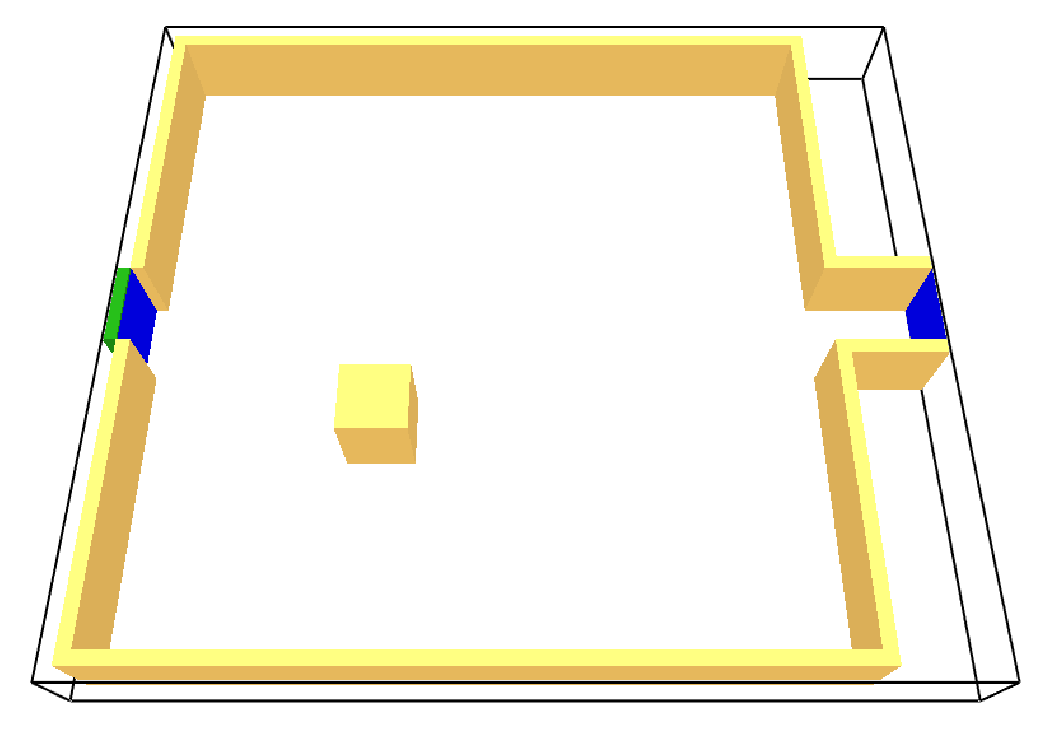
\includegraphics[clip=true,
    width=75mm]{FIGURES/evac_example1_EvacGeom} 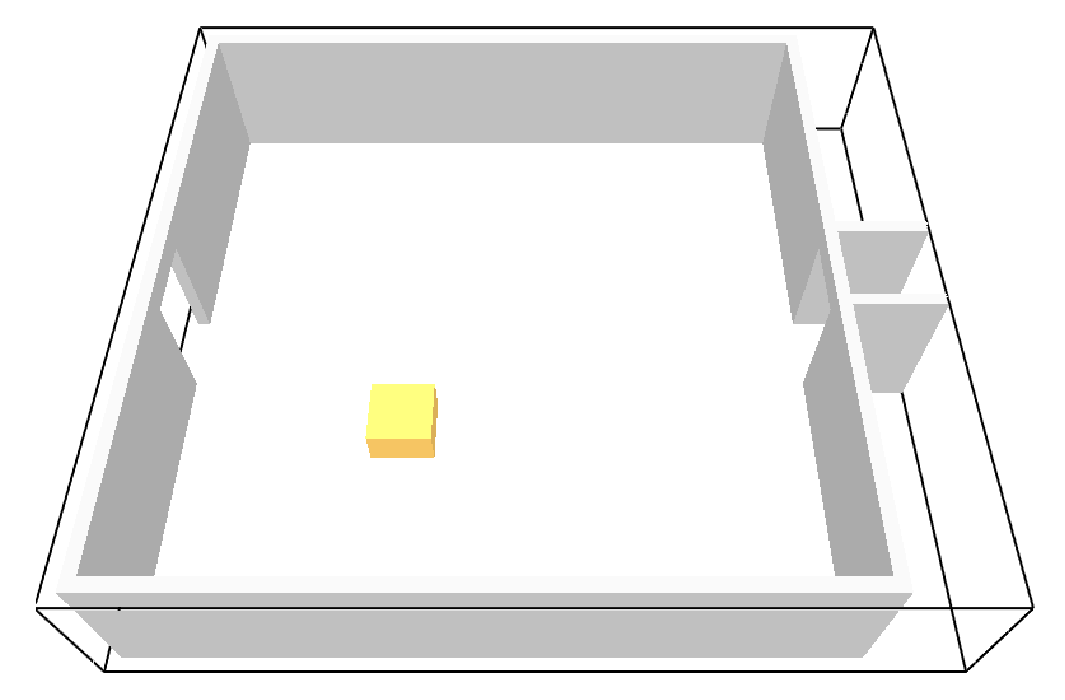
\includegraphics[clip=true,
    width=75mm]{FIGURES/evac_example1_FireGeom}}
  \caption{Example 1: Evacuation and fire calculation
    geometries.}\label{Fig_Ex1EvacGeom}
\end{figure}


The first input file specifies a fire in a room with two doors, see
Figure~\ref{Fig_Ex1EvacGeom}.  Agents are using both doors and they
select the door by using the exit door selection algorithm, thus, each
of the two doors needs its own evacuation flow field.  This means that
one needs to define the main evacuation mesh and two additional door
flow field meshes for this case besides the fire mesh.
\vspace{\fill}

{\fontsize{10}{13}
\selectfont
\begin{verbatim}
&HEAD CHID='evac_example1', TITLE='Test 1, fire+evac'  / 

 Fire mesh(es).
&MESH IJK=60,54,12, XB= -0.4,11.6, -0.4,10.4, 0.0,2.4 /

 One floor with 2 exit doors, thus, we need:
 one main evac mesh   (EVACUATION=.TRUE., EVAC_HUMANS=.TRUE.)
 two door flow meshes (EVACUATION=.TRUE., EVAC_HUMANS=.FALSE.)

 Main evacuation mesh for this floor. This mesh contains the humans.
 Evacuation meshes should all have an unique ID string defined.

&MESH IJK=60,54,1,XB=-0.4,11.6, -0.4,10.4, 0.4,1.6,EVAC_Z_OFFSET=1.0,
      EVACUATION=.TRUE., EVAC_HUMANS=.TRUE., ID='MainEvacGrid' /

 Additional door flow fields.
 Note: main evacuation mesh and the door flow meshes should have
 same XB and IJK.

&MESH IJK=60,54,1, XB= -0.4,11.6, -0.4,10.4, 0.4,1.6,
      EVACUATION=.TRUE., ID='LeftExitGrid' /
&MESH IJK=60,54,1, XB= -0.4,11.6, -0.4,10.4, 0.4,1.6, 
      EVACUATION=.TRUE., ID='RightExitGrid' /

&TIME T_END=200.0 / 

&MISC SURF_DEFAULT='WALL',
      EVAC_SURF_DEFAULT = 'EVAC_WALL' / 

&DUMP SMOKE3D=.TRUE.,
      NFRAMES=200,
      DT_PART=0.5,
      DT_HRR=1.0,
      DT_SLCF=1.0,
      DT_PL3D=100.0,
      DT_ISOF=5.0 /

&REAC ID         = 'POLYURETHANE'
      FYI        = 'C_6.3 H_7.1 N O_2.1, NFPA Handbook, Babrauskas'
      SOOT_YIELD = 0.10
      CO_YIELD   = 0.05
      N          = 1.0
      C          = 6.3
      H          = 7.1
      O          = 2.1  /

&SURF ID='BURNER', HRRPUA=1000., COLOR='RASPBERRY' /

&MATL ID            = 'GYPSUM PLASTER'
      FYI           = 'Quintiere, Fire Behavior'
      CONDUCTIVITY  = 0.48
      SPECIFIC_HEAT = 0.84
      DENSITY       = 1440. /

&SURF ID             = 'WALL'
      RGB            = 200,200,200
      MATL_ID        = 'GYPSUM PLASTER'
      THICKNESS      = 0.012 /

 Boundary condition for the evacuation flow fields:
&SURF ID='OUTFLOW', VEL = +0.000001, TAU_V=0.1 /

&SURF ID='EVAC_WALL', RGB= 200,0,200 / or COLOR

 Ordinary fire calculation geometry input.
&OBST XB= -0.20, 0.00, -0.20, 10.20, 0.00, 2.40, SURF_ID='WALL' /
&OBST XB= 10.00,10.20, -0.20, 10.20, 0.00, 2.40, SURF_ID='WALL' /
&OBST XB= -0.20,10.20, -0.20,  0.00, 0.00, 2.40, SURF_ID='WALL' /
&OBST XB= -0.20,10.20, 10.00, 10.20, 0.00, 2.40, SURF_ID='WALL' /
&OBST XB= 10.00,11.60,  4.20,  4.40, 0.00, 2.40, SURF_ID='WALL' /
&OBST XB= 10.00,11.60,  5.60,  5.80, 0.00, 2.40, SURF_ID='WALL' /
&HOLE XB= -0.21, 0.01,  4.39,  5.61, 0.00, 2.00 /
&HOLE XB=  9.99,10.21,  4.39,  5.61, 0.00, 2.00 /

 The fire as a burner.
&OBST XB= 3.00, 4.00, 3.00, 4.00, 0.00, 0.60, SURF_ID='INERT' /
&VENT XB= 3.00, 4.00, 3.00, 4.00, 0.60, 0.60, SURF_ID='BURNER' /

&VENT MB='YMIN',SURF_ID='OPEN' / 
&VENT MB='YMAX',SURF_ID='OPEN' / 

 Evacuation geometry input.

 Define the evacuation vents for the main evacuation mesh, there
 should be an evacuation vent at every place, where humans can
 go 'inside' some door, exit, etc object.
 
 This vent is not at an outer boundary of the domain nor at a solid
 object, thus, there should be an OBST behind it (FDS5 restriction).
 Left Exit:
&VENT XB= -0.20,-0.20,  4.40,5.60, 0.40,1.60, SURF_ID='OUTFLOW', 
      MESH_ID='MainEvacGrid', EVACUATION=.TRUE., RGB=0,0,255 /
&OBST XB= -0.40,-0.20,  4.40,5.60, 0.40,1.60, SURF_ID='INERT', 
      EVACUATION=.TRUE., RGB=30,150,20 / 
 
 This vent is at the outer boundary of the domain, i.e., it is
 on a solid object (by default).
 Right Exit:
&VENT XB= 11.60,11.60,  4.40,5.60, 0.40,1.60, SURF_ID='OUTFLOW', 
      MESH_ID='MainEvacGrid', EVACUATION=.TRUE., RGB=0,0,255/

 An exit namelist defines an exit door which takes humans 
 out of the calculation.
&EXIT ID='LeftExit', IOR=-1,
      FYI= 'Comment line',
      VENT_FFIELD='LeftExitGrid',
      COLOR='BLUE',
      XYZ= 0.20, 5.00, 1.00,
      XB= -0.20,-0.20,  4.40,5.60, 0.40,1.60 /
&VENT XB= -0.20,-0.20,  4.40,5.60, 0.40,1.60, SURF_ID='OUTFLOW', 
      MESH_ID='LeftExitGrid', EVACUATION=.TRUE./ Left Exit Fan

&EXIT ID='RightExit', IOR=+1,
      FYI= 'Comment line',
      VENT_FFIELD='RightExitGrid',
      COLOR='RED',
      XYZ= 11.40, 5.00, 1.00,
      XB= 11.60,11.60,  4.40,5.60, 0.40,1.60 /
&VENT XB= 11.60,11.60,  4.40,5.60, 0.40,1.60, SURF_ID='OUTFLOW', 
      MESH_ID='RightExitGrid', EVACUATION=.TRUE./ Right Exit Fan

 Next is just a counter, i.e., it just produces a column in
 the CHID_evac.csv file.
&EXIT ID='RightCounter', IOR=+1,
      FYI= 'Comment line',
      COUNT_ONLY=.TRUE.,
      XB= 10.00,10.00,  4.40,5.60, 0.40,1.60 /

 Evacuation calculation, human properties
&PERS ID='Adult',
      FYI='Male+Female diameter and velocity',
      DEFAULT_PROPERTIES='Adult',
      PRE_EVAC_DIST=1,PRE_MEAN=10.0,PRE_LOW=5.0,PRE_HIGH=15.0,
      DET_EVAC_DIST=1,DET_MEAN=10.0,DET_LOW=5.00,DET_HIGH=15.0,
      TDET_SMOKE_DENS=0.1 ,
      HUMAN_SMOKE_HEIGHT=1.6,
      DENS_INIT=4.0,
      OUTPUT_SPEED=.TRUE.,
      OUTPUT_FED=.TRUE.,
      COLOR_METHOD = 0 /

&PERS ID='Male',
      FYI='Male diameter and velocity',
      DEFAULT_PROPERTIES='Male',
      PRE_EVAC_DIST=1,PRE_MEAN=10.0,PRE_LOW=5.0,PRE_HIGH=15.0,
      DET_EVAC_DIST=1,DET_MEAN=10.0,DET_LOW=5.00,DET_HIGH=15.0 /

&PERS ID='Female',
      FYI='Female diameter and velocity',
      DEFAULT_PROPERTIES='Female',
      PRE_EVAC_DIST=1,PRE_MEAN=10.0,PRE_LOW=5.0,PRE_HIGH=15.0,
      DET_EVAC_DIST=1,DET_MEAN=10.0,DET_LOW=5.00,DET_HIGH=15.0 /

&PERS ID='Child',
      FYI='Child diameter and velocity',
      DEFAULT_PROPERTIES='Child',
      PRE_EVAC_DIST=1,PRE_MEAN=10.0,PRE_LOW=5.0,PRE_HIGH=15.0,
      DET_EVAC_DIST=1,DET_MEAN=10.0,DET_LOW=5.00,DET_HIGH=15.0 /

&PERS ID='Elderly',
      FYI='Elderly diameter and velocity',
      DEFAULT_PROPERTIES='Elderly',
      PRE_EVAC_DIST=1,PRE_MEAN=10.0,PRE_LOW=5.0,PRE_HIGH=15.0,
      DET_EVAC_DIST=1,DET_MEAN=10.0,DET_LOW=5.00,DET_HIGH=15.0 /

 Initial positions of the humans

 These humans will use the left exit, if it is not blocked by smoke.
&EVAC ID = 'HumanLeftDoorKnown', 
      NUMBER_INITIAL_PERSONS = 25,
      XB = 1.0,9.0,  1.0,9.0, 0.4,1.6
      AVATAR_COLOR = 'BLUE',
      KNOWN_DOOR_NAMES = 'LeftExit',
      KNOWN_DOOR_PROBS = 1.0,
      PERS_ID = 'Male' / 

 These humans will use the right exit, if it is not blocked by smoke.
&EVAC ID = 'HumanRightDoorKnown', 
      NUMBER_INITIAL_PERSONS = 25,
      XB = 1.0,9.0,  1.0,9.0, 0.4,1.6
      AVATAR_COLOR = 'RED',
      KNOWN_DOOR_NAMES = 'RightExit',
      KNOWN_DOOR_PROBS = 1.0,
      PERS_ID = 'Female' / 

 These humans know both doors so they will use the nearest visible
 known door which is not blocked by smoke.
&EVAC ID = 'HumanBothDoorsKnown', 
      NUMBER_INITIAL_PERSONS = 25,
      XB = 1.0,9.0,  1.0,9.0, 0.4,1.6
      AVATAR_COLOR = 'GREEN',
      KNOWN_DOOR_NAMES = 'LeftExit','RightExit',
      KNOWN_DOOR_PROBS = 1.0,1.0,
      PERS_ID = 'Child' / 

 These humans do not have a known door and they will try to go to the
 nearest visible exit door. 
&EVAC ID = 'HumanNoDoorKnown', 
      NUMBER_INITIAL_PERSONS = 25,
      XB = 1.0,9.0,  1.0,9.0, 0.4,1.6
      AVATAR_COLOR = 'BLACK',
      PERS_ID = 'Adult' / 

 An evacuation hole, e.g., do not put humans on top of the fire.
&EVHO ID = 'Evho_Fire',
      FYI = 'Do not put humans close to the fire',
      XB = 2.0,5.0, 2.0,5.0, 0.4,1.6 /

 Fire calculation output.
&BNDF QUANTITY='WALL_TEMPERATURE' / 
&SLCF PBX=2.40, QUANTITY='TEMPERATURE' /

 Next line could be used to plot the evacuation flow fields:
&SLCF PBZ=1.0, QUANTITY='VELOCITY', VECTOR=.TRUE., EVACUATION=.TRUE. / 

&TAIL /

\end{verbatim}
}


\begin{figure}[!tb]
  \centerline{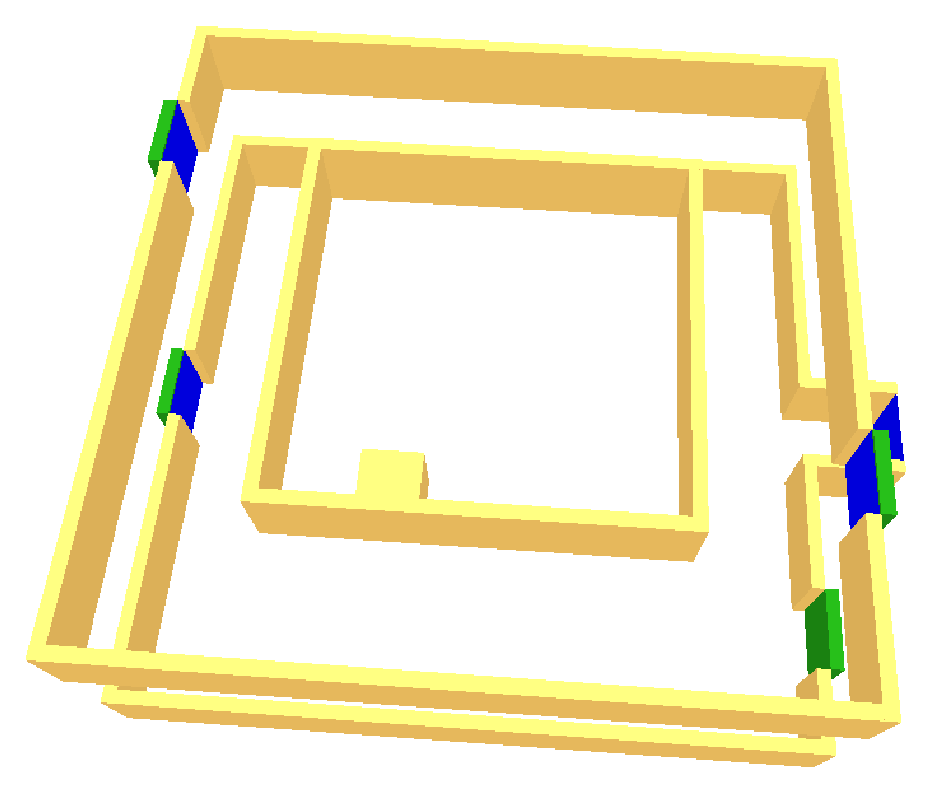
\includegraphics[clip=true,
    width=80mm]{FIGURES/evac_example2_EvacGeom}}
  \caption{Example 2: Evacuation calculation
    geometry.}\label{Fig_Ex2EvacGeom}
\end{figure}

The second input file specifies a two-floor building, see
Figure~\ref{Fig_Ex2EvacGeom}, each floor consisting of one egress area,
thus only one main evacuation mesh per floor is needed.  There is a
fire in downstairs and the smoke is going to the second floor by an
opening at the ceiling.  The second floor is connected to the first
floor in the egress calculation, \emph{i.e.}, the second floor agents
are transfered to the first floor by the combination of doors and
stairs.  The second floor has two exit doors, one leading to the
stairs going to the first floor (the right exit door) and one leading
to the stairs leading directly to outside of the building (the left
exit).  The first floor has two exit doors and one entry, which the
agents from the second floor are using when entering the first floor.

{\fontsize{10}{13}
\selectfont
\begin{verbatim}
&HEAD CHID='evac_example2', TITLE='Test 2, fire+evac'  / 

 Fire mesh(es).
&MESH IJK=54,50,25, XB= -0.2,10.6,  0.0,10.0, 0.0,5.0 /

 Main evacuation meshes for the floors. These meshes contains the
 humans. Evacuation meshes should all have an unique ID string 
 defined.

&MESH IJK=60,54,1,XB=-0.4,11.6, -0.4,10.4, 0.4,1.6,EVAC_Z_OFFSET=1.0,
      EVACUATION=.TRUE., EVAC_HUMANS=.TRUE., ID='MainEvacGrid' /
&MESH IJK=54,54,1,XB=-0.4,10.4, -0.4,10.4, 3.0,4.2,EVAC_Z_OFFSET=1.0,
      EVACUATION=.TRUE., EVAC_HUMANS=.TRUE., ID='MainEvacGrid2' /

 Additional door flow fields.
 Note: main evacuation grid and the door flow grids should have
 same XB and IJK.

&MESH IJK=60,54,1, XB= -0.4,11.6, -0.4,10.4, 0.4,1.6,
      EVACUATION=.TRUE., ID='LeftExitGrid' / Left, 1st floor
&MESH IJK=60,54,1, XB= -0.4,11.6, -0.4,10.4, 0.4,1.6, 
      EVACUATION=.TRUE., ID='RightExitGrid' / Right, 1st floor

&MESH IJK=54,54,1, XB= -0.4,10.4, -0.4,10.4, 3.0,4.2,
      EVACUATION=.TRUE., ID='LeftDoorGrid2' / Left, 2nd floor
&MESH IJK=54,54,1, XB= -0.4,10.4, -0.4,10.4, 3.0,4.2, 
      EVACUATION=.TRUE., ID='RightDoorGrid2' / Right, 2nd floor

&TIME T_END=200.0 / 

&MISC SURF_DEFAULT='WALL',
      EVAC_SURF_DEFAULT= 'EVAC_WALL' / 

&DUMP SMOKE3D=.TRUE.,
      NFRAMES=200,
      DT_PART=0.5,
      DT_HRR=1.0,
      DT_SLCF=1.0,
      DT_BNDF=5.0,
      DT_PL3D=100.0,
      DT_ISOF=5.0 /

&REAC ID         = 'POLYURETHANE'
      FYI        = 'C_6.3 H_7.1 N O_2.1, NFPA Handbook, Babrauskas'
      SOOT_YIELD = 0.10
      N          = 1.0
      C          = 6.3
      H          = 7.1
      O          = 2.1  /

&SURF ID='BURNER', HRRPUA=1000., COLOR='RASPBERRY' /

&MATL ID            = 'GYPSUM PLASTER'
      FYI           = 'Quintiere, Fire Behavior'
      CONDUCTIVITY  = 0.48
      SPECIFIC_HEAT = 0.84
      DENSITY       = 1440. /

&SURF ID             = 'WALL'
      RGB            = 200,200,200
      MATL_ID        = 'GYPSUM PLASTER'
      THICKNESS      = 0.012 /

 Boundary condition for the evacuation flow fields:
&SURF ID = 'OUTFLOW', VEL = +0.000001, TAU_V=0.1 /

&SURF ID = 'EVAC_WALL', RGB= 200,0,200 / or COLOR

 Ordinary fire calculation geometry input.
&OBST XB= -0.20,10.20, -0.20, 10.20, 2.40, 2.60 / floor
&HOLE XB=  2.20, 7.80,  2.20,  7.80, 2.39, 2.61 / floor hole
&OBST XB=  2.00, 8.00,  2.00,  2.20, 2.60, 3.60 / balustrade
&OBST XB=  2.00, 8.00,  7.80,  8.00, 2.60, 3.60 / balustrade
&OBST XB=  2.00, 2.20,  2.00,  8.00, 2.60, 3.60 / balustrade
&OBST XB=  7.80, 8.00,  2.00,  8.00, 2.60, 3.60 / balustrade
&OBST XB= 10.20,11.60,  4.20,  5.80, 2.40, 2.60 / floor

&OBST XB= -0.20, 0.00, -0.20, 10.20, 0.00, 5.00 /
&OBST XB= 10.00,10.20, -0.20, 10.20, 0.00, 5.00 /
&OBST XB= -0.20,10.20, -0.20,  0.00, 0.00, 5.00 /
&OBST XB= -0.20,10.20, 10.00, 10.20, 0.00, 5.00 /
&OBST XB= 10.00,11.60,  4.20,  4.40, 0.00, 2.40 / Right Corridor Wall
&OBST XB= 10.00,11.60,  5.60,  5.80, 0.00, 2.40 / Right Corridor Wall
&HOLE XB= -0.21, 0.01,  4.39,  5.61, 0.00, 2.00 / Left Door
&HOLE XB=  9.99,10.21,  4.39,  5.61, 0.00, 2.00 / Right Door Hole

 The fire as an burner.
&OBST XB= 3.00, 4.00, 3.00, 4.00, 0.00, 0.60, SURF_ID='INERT' /
&VENT XB= 3.00, 4.00, 3.00, 4.00, 0.60, 0.60, SURF_ID='BURNER' /

&VENT MB='YMIN',SURF_ID='OPEN' / 
&VENT MB='YMAX',SURF_ID='OPEN' / 

 Evacuation geometry input.

&HOLE XB= -0.21, 0.01,  7.39,  8.61, 2.60, 4.60, EVACUATION=.TRUE. /
&HOLE XB=  9.99,10.21,  2.39,  3.61, 2.60, 4.60, EVACUATION=.TRUE. /

 Define the evacuation vents for the main evacuation meshes, there
 should be an evacuation vent at every place, where humans can
 go 'inside' some door, exit, etc object.

 This vent is not at an outer boundary of the domain nor at a solid
 object, thus, there should be an OBST behind it (FDS5 restriction).
 Left Exit, 1st Floor:
&VENT XB= -0.20,-0.20,  4.40,5.60, 0.40,1.60, SURF_ID='OUTFLOW', 
      MESH_ID='MainEvacGrid', EVACUATION=.TRUE., RGB=0,0,255 /
&OBST XB= -0.40,-0.20,  4.40,5.60, 0.40,1.60, 
      EVACUATION=.TRUE., RGB=30,150,20 / 

 This vent is at the outer boundary of the domain, i.e., it is
 on a solid object (by default).
 Right Exit, 1st Floor:
&VENT XB= 11.60,11.60,  4.40,5.60, 0.40,1.60, SURF_ID='OUTFLOW', 
      MESH_ID='MainEvacGrid', EVACUATION=.TRUE., RGB=0,0,255 /

 This vent is not at an outer boundary of the domain nor at a solid
 object, thus, there should be an OBST behind it.
 Right Exit, 2nd Floor:
&VENT XB= 10.20,10.20,  2.40,3.60, 3.0,4.2, SURF_ID='OUTFLOW', 
      MESH_ID='MainEvacGrid2', EVACUATION=.TRUE., RGB=0,0,255 /
&OBST XB= 10.20,10.40,  2.40,3.60, 3.0,4.2, 
      EVACUATION=.TRUE., RGB=30,150,20 / Right Door, 2nd

 This vent is not at an outer boundary of the domain nor at a solid
 object, thus, there should be an OBST behind it.
 Left Exit, 2nd Floor:
&VENT XB= -0.20,-0.20,  7.40,8.60, 3.0,4.2, SURF_ID='OUTFLOW', 
      MESH_ID='MainEvacGrid2', EVACUATION=.TRUE., RGB=0,0,255 /
&OBST XB= -0.40,-0.20,  7.40,8.60, 3.0,4.2, 
      EVACUATION=.TRUE., RGB=30,150,20 / Left Door, 2nd

 An exit namelist defines an exit door which takes humans out
 of the calculation.
&EXIT ID='LeftExit', IOR=-1,
      FYI= 'Comment line',
      VENT_FFIELD='LeftExitGrid',
      COLOR='BLUE',
      XYZ= 0.20, 5.00, 1.00,
      XB= -0.20,-0.20,  4.40,5.60, 0.40,1.60 /
&VENT XB= -0.20,-0.20,  4.40,5.60, 0.40,1.60, SURF_ID='OUTFLOW', 
      MESH_ID='LeftExitGrid', EVACUATION=.TRUE./ Left Exit Fan

&EXIT ID='RightExit', IOR=+1,
      FYI= 'Comment line',
      VENT_FFIELD='RightExitGrid',
      COLOR='RED',
      XYZ= 11.40, 5.00, 1.00,
      XB= 11.60,11.60,  4.40,5.60, 0.40,1.60 /
&VENT XB= 11.60,11.60,  4.40,5.60, 0.40,1.60, SURF_ID='OUTFLOW', 
      MESH_ID='RightExitGrid', EVACUATION=.TRUE./ Right Exit Fan

 Next is just a counter, i.e., it just produces a column in
 the CHID_evac.csv file.
&EXIT ID='RightCounter', IOR=+1,
      FYI= 'Comment line',
      COUNT_ONLY=.TRUE.,
      XB= 10.00,10.00,  4.40,5.60, 0.40,1.60 /

 Second floor doors etc.

 This is a combination of a door leading to a stairs, which is
 leading directly to outside of the building: 
 DOOR ==> CORR ==> EXIT combination.
&DOOR ID='LeftDoor2nd', IOR=-1,
      FYI= 'Comment line',
      VENT_FFIELD='LeftDoorGrid2',
      COLOR='GREEN',
      EXIT_SIGN=.TRUE.,
      TO_NODE= 'LeftCorr'
      XYZ= 0.2, 8.00, 3.6,
      XB= -0.20,-0.20, 7.40,8.60, 3.0,4.2 /
&VENT XB= -0.20,-0.20, 7.40,8.60, 3.0,4.2 SURF_ID='OUTFLOW', 
      MESH_ID='LeftDoorGrid2', EVACUATION=.TRUE./ Left Door Fan, 2nd
&CORR ID='LeftCorr',
      FYI='Comments',
      MAX_HUMANS_INSIDE=20,
      EFF_LENGTH= 8.5,
      FAC_SPEED=0.7,
      TO_NODE='LeftCorrExit' /
&EXIT ID='LeftCorrExit',
      FYI='A dummy exit, the end point to a corridor object',
      IOR=-1,
      XB= -0.40,-0.40, 7.40,8.60, 0.40,1.60 /

 This is a combination of a door leading to a stairs, which is
 leading to the first floor: DOOR ==> CORR ==> ENTR combination.
&DOOR ID='RightDoor2nd', IOR=+1,
      FYI= 'Comment line',
      VENT_FFIELD='RightDoorGrid2',
      TO_NODE= 'RightCorr'
      COLOR='MAGENTA',
      EXIT_SIGN=.TRUE.,
      XYZ= 9.8, 3.00, 3.6,
      XB= 10.20,10.20, 2.40,3.60, 3.0,4.2 /
&VENT XB= 10.20,10.20, 2.40,3.60, 3.0,4.2, SURF_ID='OUTFLOW', 
      MESH_ID='RightDoorGrid2', EVACUATION=.TRUE./ 
&CORR ID='RightCorr',
      FYI='Comments',
      MAX_HUMANS_INSIDE=20,
      EFF_LENGTH= 8.5,
      FAC_SPEED=0.7,
      TO_NODE='RightEntry' /
&ENTR ID='RightEntry',
      FYI='Comments',
      IOR=-1,
      XB=10.20,10.20,  1.00,2.20,  0.40,1.60 /
&HOLE XB= 9.99,10.21,  1.00,2.20,  0.40,1.60, 
      EVACUATION=.TRUE., RGB=30,150,20 / 1st Floor Entry
&OBST XB=10.20,10.40,  1.00,2.20,  0.40,1.60, 
      EVACUATION=.TRUE., RGB=30,150,20 / 1st Floor Entry

 Evacuation calculation, human properties

&PERS ID='Adult',
      FYI='Male+Female diameter and velocity',
      DEFAULT_PROPERTIES='Adult',
      PRE_EVAC_DIST=1,PRE_MEAN=10.0,PRE_LOW=5.0,PRE_HIGH=15.0,
      DET_EVAC_DIST=1,DET_MEAN=10.0,DET_LOW=5.00,DET_HIGH=15.0,
      TDET_SMOKE_DENS=0.1 ,
      HUMAN_SMOKE_HEIGHT=1.6,
      DENS_INIT= 4.0,
      OUTPUT_SPEED=.TRUE.,
      OUTPUT_FED=.TRUE.,
      COLOR_METHOD = 0 /

&PERS ID='Male',
      FYI='Male diameter and velocity',
      DEFAULT_PROPERTIES='Male',
      PRE_EVAC_DIST=1,PRE_MEAN=10.0,PRE_LOW=5.0,PRE_HIGH=15.0,
      DET_EVAC_DIST=1,DET_MEAN=10.0,DET_LOW=5.00,DET_HIGH=15.0 /

&PERS ID='Female',
      FYI='Female diameter and velocity',
      DEFAULT_PROPERTIES='Female',
      PRE_EVAC_DIST=1,PRE_MEAN=10.0,PRE_LOW=5.0,PRE_HIGH=15.0,
      DET_EVAC_DIST=1,DET_MEAN=10.0,DET_LOW=5.00,DET_HIGH=15.0 /

&PERS ID='Child',
      FYI='Child diameter and velocity',
      DEFAULT_PROPERTIES='Child',
      PRE_EVAC_DIST=1,PRE_MEAN=10.0,PRE_LOW=5.0,PRE_HIGH=15.0,
      DET_EVAC_DIST=1,DET_MEAN=10.0,DET_LOW=5.00,DET_HIGH=15.0 /

&PERS ID='Elderly',
      FYI='Elderly diameter and velocity',
      DEFAULT_PROPERTIES='Elderly',
      PRE_EVAC_DIST=1,PRE_MEAN=10.0,PRE_LOW=5.0,PRE_HIGH=15.0,
      DET_EVAC_DIST=1,DET_MEAN=10.0,DET_LOW=5.00,DET_HIGH=15.0 /

 Initial positions of the humans

 1st Floor:
 These humans will use the left exit, if it is not blocked by smoke.
&EVAC ID = 'HumanLeftDoorKnown', 
      NUMBER_INITIAL_PERSONS = 25,
      XB = 1.0,9.0,  1.0,9.0, 0.4,1.6
      AVATAR_COLOR = 'BLUE',
      KNOWN_DOOR_NAMES = 'LeftExit',
      KNOWN_DOOR_PROBS = 1.0,
      PERS_ID = 'Male' / 

 These humans will use the right exit, if it is not blocked by smoke.
&EVAC ID = 'HumanRightDoorKnown', 
      NUMBER_INITIAL_PERSONS = 25,
      XB = 1.0,9.0,  1.0,9.0, 0.4,1.6
      AVATAR_COLOR = 'RED',
      KNOWN_DOOR_NAMES = 'RightExit',
      KNOWN_DOOR_PROBS = 1.0,
      PERS_ID = 'Female' / 

 These humans know both doors so they will use the nearest visible
 known door which is not blocked by smoke.
&EVAC ID = 'HumanBothDoorsKnown', 
      NUMBER_INITIAL_PERSONS = 25,
      XB = 1.0,9.0,  1.0,9.0, 0.4,1.6
      AVATAR_COLOR = 'GREEN',
      KNOWN_DOOR_NAMES = 'LeftExit','RightExit',
      KNOWN_DOOR_PROBS = 1.0,1.0,
      PERS_ID = 'Child' / 

 These humans do not have a known door and they will try to go to
 the nearest visible exit door. 
&EVAC ID = 'HumanNoDoorKnown', 
      NUMBER_INITIAL_PERSONS = 25,
      XB = 1.0,9.0,  1.0,9.0, 0.4,1.6
      AVATAR_COLOR = 'BLACK',
      PERS_ID = 'Adult' / 

 2nd Floor:
 All of these humans know the right door on the 2nd floor and the
 right exit on the first floor. On the average, only 50 \% know
 the left door on the second floor and none knows the left exit
 on the first floor.
&EVAC ID = 'Human2ndFloor', 
      NUMBER_INITIAL_PERSONS = 50,
      XB = 0.5,9.5,  0.5,9.5, 3.0,4.2
      AVATAR_COLOR = 'MAGENTA',
      KNOWN_DOOR_NAMES = 'LeftDoor2nd','RightDoor2nd','RightExit',
      KNOWN_DOOR_PROBS = 0.5,1.0,1.0,
      PERS_ID = 'Adult' / 

 An evacuation hole, e.g., do not put humans on top of the fire.
&EVHO ID = 'Evho_Fire',
      FYI = 'Do not put humans close to the fire',
      XB = 2.0,5.0, 2.0,5.0, 0.4,1.6 /

 An evacuation hole, e.g., do not put humans on top of the opening
 in the ceiling.
&EVHO ID = 'Evho_2ndFloor',
      FYI = 'atrium space',
      XB = 2.0,8.0, 2.0,8.0, 3.0,4.2 /

 Fire calculation output.
&BNDF QUANTITY='WALL_TEMPERATURE' / 
&SLCF PBX=2.40, QUANTITY='TEMPERATURE' /

 Next lines could be used to plot the evacuation flow fields:
&SLCF PBZ=1.0, QUANTITY='VELOCITY', VECTOR=.TRUE., EVACUATION=.TRUE. / 
&SLCF PBZ=3.6, QUANTITY='VELOCITY', VECTOR=.TRUE., EVACUATION=.TRUE. / 

&TAIL /
\end{verbatim}
}

\clearpage

\newpage

\chapter{Conclusion}\label{Sec_Conclusions}

The development work of FDS+Evac is an undergoing project.  Read
carefully through the Chapters \ref{Sec_SpecFeatures} and
\ref{Sec_UsesAndLimit} of this guide, where the features and
limitations of the current version of the programme are listed.  Read
also Ch.~\ref{Sec_RecentChanges} and the \Timtt{Readme.txt} file on
the FDS+Evac web pages to see the latest changes to the user inputs.
The development work of FDS+Evac is nicely summarised on the VTT's
project summary report~\cite{Hostikka07a}.  The verification and
validation work of FDS+Evac is reported on this manual and some
additional work is presented on the FDS+Evac web pages at
\texttt{http://www.vtt.fi/fdsevac/}.

The present status of the FDS+Evac (FDS 5.3.0, Evac 2.1.1) is:
%
\begin{itemize}
%
\item Smoke vs walking speed correlations are included.
%
\item Fractional Effective Dose is calculated and used to
  'incapacitate' agents, but only CO, CO${}_\mathrm{2}$ and
  O${}_\mathrm{2}$ concentrations are used.
%
\item Smoke density can be used to trigger agent movement (detection
  by smoke).
%
\item A simple exit door selection algorithm is implemented.
%
\item Inclines, stairs, and escalators can be modelled explicitly by
  using the equations of motion for each person.
%
\item A simple stairs algorithm without merging flows is implemented.
  If there are merging flows in stairs then these should be modelled
  explicitly, which means some additional work to construct the input
  file containing the landings and stairs using.
%
\item The flows through doors, stairs and corridors are reproduced
  nicely by the underlying dynamics.
%
\item Congestion can be studied.
%
\item The effect of the many input parameters of the agent movement
  model are understood well and their effect on the specific flows is
  known.
%
\end{itemize}
%

Below the TO DO list of the development work of FDS+Evac is
presented.  Note that some of the items on the list are already added
to the programme source code but these are not discussed on this
manual.  These features are still work-on-progress stage.
%
\begin{itemize}
%
\item Merging flows in stairs: An easy to use staircase model with
  merging flows and smoke information is implemented and it is now in
  V\&V phase.  
%
\item More predefined human types, especially those referred in the
  IMO circular~\cite{IMO02}.
%
\item More intelligence in the exit door selection algorithm,
  \emph{e.g.}, estimated queueing time due to the other agents
  heading/queueing for the same exit door, which is already implemented
  and it is on a testing phase.  Better treatment of the
  non-visible known doors.
%
\item Social interactions like herding, small groups, \emph{etc.}.  A
  small group feature is already implemented but it is not yet validated.
%
\item Spreading of the information: agent to agent communication like
  fire detection.
%
\item Easier generation of the input file.
%
\item Counterflow is implemented but need still V\&V work.
%
\item More optimal computer memory usage.
%
\item Parallelisation of the evacuation calculation using MPI/OpenMPI.
%
\end{itemize}
%


\noindent The shortcomings of FDS+Evac are:
%
\begin{itemize}
%
\item Restrictions on the geometry and the computational mesh due to
  the rectangular nature of the FDS geometry, \emph{i.e.}, objects,
  whose edges are along the $x$ and $y$, are the main elements used to
  construct the geometry, including inclines and stairs.
%
\item Merging flows in stairs are not easy to model.
%
\item No elevators.
%
\item The evacuation objects, like exits, doors, \emph{etc.}, are not
  visualised on the Smokeview window.
%
\item The user input is not easy to give, \emph{i.e.}, no support for
  importing CAD drawings for the evacuation calculation.  There exists
  commercial software tools that generate FDS fire input and these
  tools can be used to generate an FDS model of the building. 
%
\item CPU and RAM memory intensive.
%
\end{itemize}
%

Users should notice that the evacuation part of FDS5 is under
development, and the features and user input may change in the future.
Thus, one should always use the latest version of FDS, which can be
downloaded from \emph{http://www.fire.nist/fds/downloads.html}.  One
should also check the FDS+Evac web pages at
\emph{http://www.vtt.fi/fdsevac/} for the latest version of this
manual.  This page also contains more verification and validation
results and example cases than this manual and the example files there
are ``up to date'' with the most resent version of the programme.


\clearpage

\newpage

\chapter*{Acknowledgements}
\addcontentsline{toc}{chapter}{Acknowledgements}

The Evacuation Module of the Fire Dynamics Simulator has been under
development for some years.  Dr.\ Kevin McGrattan of NIST is
acknowledged for helping to implement the evacuation subroutine in the
FDS code and Dr.\ Glenn Forney of NIST is acknowledged for the
modifications needed in the visualisation program Smokeview.
University of Helsinki and Helsinki University of Technology are
acknowledged for the cooperation.

The development work of FDS+Evac has been funded by the VTT Technical
Research Centre of Finland, the Finnish Funding Agency for Technology
and Innovation, the Finnish Fire Protection Fund, the Ministry of the
Environment, and the Academy of Finland.  The Building and Fire
Research Laboratory at NIST is acknowledged for the hospitality during
the visits of one of the authors (T.K.).

\clearpage

\newpage

\addcontentsline{toc}{chapter}{References}
\renewcommand{\bibname}{References}
\begin{thebibliography}{99}
%
%
\bibitem{FDS_Manual} McGrattan, K., Hostikka, S., Floyd, J., Baum, H.,
  and Rehm, R., ``Fire Dynamics Simulator (Version 5) Technical
  Reference Guide Volume 1: Mathematical Model'', NIST Special
  Publication 1018-5, National Institute of Standards and
  Technology, Gaithersburg, MA, July 2008, 92~p.
%
\bibitem{FDS_UserGuide} McGrattan, K., Klein, B., Hostikka, S., and
  Floyd, J., ``Fire Dynamics Simulator (Version 5) User's Guide'',
  NIST Special Publication 1019-5, National Institute of Standards and
  Technology, Gaithersburg, MA, July 2008, 188~p.
%
\bibitem{FDS_VVGuide1} McGrattan, K., McDermott, R., Hostikka, S., K.,
  and Floyd, J., ``Fire Dynamics Simulator (Version 5) Technical
  Reference Guide Volume 2: Verification'', NIST Special Publication
  1018-5, National Institute of Standards and Technology,
  Gaithersburg, MA, July 2008, 23~p.
%
\bibitem{FDS_VVGuide2} McGrattan, Hostikka, S., K., Floyd, J., and
  Klein, B., ``Fire Dynamics Simulator (Version 5) Technical Reference
  Guide Volume 3: Validation'', NIST Special Publication 1018-5,
  National Institute of Standards and Technology, Gaithersburg, MA,
  July 2008, 171~p.
%
\bibitem{Korhonen05} Korhonen, T., Hostikka, S., and Keski-Rahkonen,
  O., ``A Proposal for the Goals and New Techniques of Modelling
  Pedestrian Evacuation in Fires'',  \emph{Fire Safety Science} 7:
  pp.~557--567 (2005). 
%
\bibitem{Korhonen07a} Korhonen, T., Hostikka, S., Heli\"ovaara, S.,
  Ehtamo, H., and Matikainen, K., ``Integration of an Agent Based
  Evacuation Simulation and the State-of-the-Art Fire Simulation'',
  Proceedings of the 7th Asia-Oceania Symposium on Fire Science \&
  Technology, 20--22 September, 2007, Hong Kong, (in print).
%
\bibitem{Korhonen07b} Korhonen, T., Hostikka, S., Heli\"ovaara, S.,
  Ehtamo, H., and Matikainen, K., ``FDS+Evac: Evacuation Module for
  Fire Dynamics Simulator'', Proceedings of the Interflam2007: 11th
  International Conference on Fire Science and Engineering,
  Interscience Communications Limited, London, UK, pp.~1443--1448
  (2007).
%
\bibitem{Korhonen08a} Korhonen, T., Hostikka, S., Heli\"ovaara, S.,
  and Ehtamo, H., ``FDS+Evac: Modelling Social Interactions in Fire
  Evacuation'', Proceedings of the 7th International Conference on
  Performance-Based Codes and Fire Safety Design Methods, SFPE,
  Bethesda, MD, USA, pp.~241--250 (2008).
%
\bibitem{Korhonen08b} Korhonen, T., Hostikka, S., Heli\"ovaara, S.,
  and Ehtamo, H., ``FDS+Evac: An Agent Based Fire Evacuation Model'',
  Proceedings of the 4th International Conference on Pedestrian and
  Evacuation Dynamics, February 27--29, 2008, Wuppertal, Germany.
%
\bibitem{Hostikka07a} Hostikka, S., Korhonen, T., Paloposki, T.,
  Rinne, T., Heli\"ovaara, S., and Matikainen, K., ``Development and
  Validation of FDS+Evac for Evacuation Simulations, Project Summary
  Report'', VTT Research Notes 2421, VTT Technical Research Centre of
  Finland, 2007, 64~p. (http://www.vtt.fi/publications/index.jsp)
%
\bibitem{Hostikka07b} Hostikka, S., Paloposki, T., Rinne, T., Saari,
  J.-M., Korhonen, T., and Heli\"ovaara, S., ``Experimental
  Observations of Evacuation Situations'', VTT Working Papers 85, VTT
  Technical Research Centre of Finland, 2007, 52~p.
  (http://www.vtt.fi/publications/index.jsp)
%
\bibitem{SV_UserGuide} Forney, G.P., ``User's Guide for Smokeview
  Version 5 -- A Tool for Visualizing Fire Dynamics Simulation Data'',
  NIST Special Publication 1017-1, U.S.~Government Printing Office,
  Washington, 2007, 134~p.
%
\bibitem{Helbing95} Helbing, D., and Moln\'ar, P., ``Social force
  model for pedestrian dynamics'', \emph{Physical Review E} 51:
  4282--4286 (1995).
%
\bibitem{Helbing00} Helbing, D., Farkas, I., and Vicsek, T.,
  ``Simulating dynamical features of escape panic'', \emph{Nature}
  407: 487--490 (2000).
%
% Next is for book
\bibitem{Helbing02} Helbing, D., Farkas, I., Moln\'ar, P., and
  Vicsek,T., ``Simulating of Pedestrian Crowds in Normal and
  Evacuation Situations'', \emph{Pedestrian and Evacuation Dynamics},
  Schreckenberg, M. and Sharma, S.D. (eds.), Springer, Berlin, 2002,
  pp.~21--58.
%
\bibitem{Werner03} Werner, T., and Helbing, D., ``The social force
  pedestrian model applied to real life scenarios'', \emph{Pedestrian
    and Evacuation Dynamics -- Proceedings of the Seconnd International
    Conference}, University of Greenwich, London, 2003, pp.~17--26.
%
\bibitem{Langston06} Langston, P.A., Masling, R., and Asmar, B.N.,
  ``Crowd dynamics discrete element multi-circle model'', \emph{Safety
    Science} 44: 395--417 (2006).
%
\bibitem{Langston09} Smith, A., James, C., Jones, R., Langston, P.,
  Lester, E., and Drury, J., ``Modelling contra-flow in crowd dynamics
  DEM simulation'', \emph{Safety Science} 47: 395--404 (2009).
%
\bibitem{Simulex96} ``Simulex: Evacuation Modelling Software, User's
  Guide'', Integrated Environmental Solutions Ltd., Glasgow, Scotland,
  UK, 1996, 48~p.
%
\bibitem{Pan06} Pan, X., ``Computational Modeling of Human and Social
  Behaviors for Emergency Egress Analysis'', 127~p., PhD Thesis,
  Stanford University, CA, 2006.
%
\bibitem{Thompson95a} Thompson, P.A., and Marchant, E.W., ``A Computer
  Model for the Evacuation of Large Building Populations'', \em Fire
  Safety Journal \em 24: 131--148 (1995).
%
\bibitem{Thompson95b} Thompson, P.A., and Marchant, E.W., ``Testing
  and Application of the Computer Model 'Simulex''', \em Fire Safety
  Journal \em 24: 149--166 (1995).
%
\bibitem{Thompson03} Thompson, P., Lindstrom, H., Ohlsson, P., and
  Thompson, S., ``Simulex: Analysis and Changes for IMO Compliance'',
  Proceedings of 2nd International Conference: Pedestrian and
  Evacuation Dynamics, pp.~173--184 (2003).
%
\bibitem{Purser95} Purser, D.A., ``Toxicity Assessment of Combustion
  Products'', in \emph{SFPE Handbook of Fire Protection Engineering},
  2${}^\textrm{nd}$ ed., pp.~2/28--2/146, National Fire Protection
  Association, Quincy, MA, 1995.
%
\bibitem{Frantzich03} Frantzich, H., and Nilsson, D., ``Utrymning
  genom t�t r\"ok: beteende och f\"orflyttning'', 75~p., Report 3126,
  Department of Fire Safety Engineering, Lund University, Sweden,
  2003.
%
\bibitem{Jin78} Jin, T., ``Visibility through Fire Smoke'',
  \emph{Journal of Fire \& Flammability}, 9: 135--155, 1978.
%
\bibitem{Heliovaara08} Heli\"ovaara, S., Ehtamo, H., Korhonen, T., and
  Hostikka, S., ``Modeling Evacuees' Exit Selection with Best-Response
  Dynamics'', Proceedings of the 4th International Conference on
  Pedestrian and Evacuation Dynamics, February 27--29, 2008,
  Wuppertal, Germany.
%
\bibitem{Proulx1993} Proulx, G., ``A Stress Model for People Facing a
  Fire'', \emph{Journal of Environmental Psychology} 13: 137--147,
  1993.
%
%\bibitem{Fang03} Fang, Z., Lo, S.M.\ and Lu, J.A., ``On the
%  Relationship between Crowd Density and Movement Velocity'',
%  \emph{Fire Safety Journal} 38: 271--283, 2003.
%
\bibitem{IMO02} IMO, ``Interim guidelines for evacuation analyses for
  new and existing passenger ships'', MSC/Circ.1033, International
  Maritime Organization, London, 6 June 2002.
%
\bibitem{Vattulainen02} Vattulainen, I., Karttunen, M., Besold, G.,
  and Polson, J.M., ``Integration Schemes for Dissipative Particle
  Dynamics Simulations: From Softly Interacting Systems Towards Hybrid
  Models'', \emph{Journal of Chemical Physics} 116: 3967--3979, 2002.
%
\bibitem{Daamen04} Daamen, W., ``Modelling Passenger Flows in Public
  Transport Facilities'', 377~p., PhD Thesis, Delft University of
  Technology, The Netherlands, 2004 (ISBN 90-407-2521-7).
%
\bibitem{Paloposki02} Paloposki, T., Myllym\"aki, J., and Weckman, H.,
  ``Application of reliability techniques for calculation of the
  evacuation safety of a sports hall'', VTT Research Notes 2281, VTT
  Building and Transport, Espoo, Finland, 2002, 53~p.~+ app.\ 13~p. (in
  Finnish).
%
\bibitem{Exodus3} Gwynne, S., Galea, E.R., Lawrence, P., and
  Filippidis, L., ``buildingEXODUS technical manual V4.00'', 2004.
%
\bibitem{Heliovaara07} Heli\"ovaara, S., ``Computational Models for
  Human Behavior in Fire Evacuations'', M.Sc.\ Thesis, Department of
  Engineering Physics and Mathematics, Helsinki University of
  Technology, 2007 (http://www.sal.hut.fi/Publications/t-index.html).
%
\bibitem{Matikainen07} Matikainen, K., ``K\"aytt\"aytyminen
  uhkatilanteessa: Poistumisreitin valintaan vaikuttavat
  sosiaalipsykologiset tekij\"at tulipalossa'', M.Sc.\ Thesis, Faculty
  of Social Sciences, University of Helsinki, 2007 (in Finnish).
%
\end{thebibliography}

\end{document}
